\documentclass[11pt]{article}

% ---------------------------------------------------------------------
% Standard packages
% ---------------------------------------------------------------------
\usepackage[margin=1in]{geometry}       % Adjust margins cleanly
\usepackage[utf8]{inputenc}             % Proper encoding
\usepackage[T1]{fontenc}                % Better font encoding
\usepackage{setspace}                   % For line spacing if needed

% ---------------------------------------------------------------------
% Math and symbols
% ---------------------------------------------------------------------
\usepackage{amsmath, amssymb, amsfonts, mathtools}
\usepackage{mathrsfs}                   % Script math fonts

% ---------------------------------------------------------------------
% Figures and tables
% ---------------------------------------------------------------------
\usepackage{graphicx}                   % For including graphics
\usepackage{subcaption}                 % For subfigures
\usepackage{booktabs, threeparttable}   % For nice tables
\usepackage{multirow, array}            % For complex table layouts
\usepackage{caption}                    % Custom caption formatting
\usepackage{float}                      % Better float handling
\usepackage{changepage}                 % For adjusting table/figure widths

% ---------------------------------------------------------------------
% Colors and highlighting
% ---------------------------------------------------------------------
\usepackage{xcolor, soul}

% ---------------------------------------------------------------------
% References / citations
% ---------------------------------------------------------------------
\usepackage[authoryear,round]{natbib}   % Author-year citation style
\bibliographystyle{apalike}             % APA-like reference formatting

% ---------------------------------------------------------------------
% Misc
% ---------------------------------------------------------------------
\usepackage{url}                        % For URLs in references

% ---------------------------------------------------------------------
% Line spacing and paragraph spacing
% ---------------------------------------------------------------------
\setstretch{1.2}                        % Adjust line spacing (e.g., 1.2)
\setlength{\parskip}{0.8em}             % Add space between paragraphs
\setlength{\parindent}{0pt}             % No paragraph indentation

\usepackage{fancyhdr}
\DeclareMathAlphabet{\mathpzc}{OT1}{pzc}{m}{it} \DeclareMathAlphabet{\mathfrak}{U}{euf}{m}{n}
 \vspace{5mm} \setlength{\topmargin}{-.5in} \setlength{\textheight}{8.85in}
\setlength{\oddsidemargin}{-.02in} \setlength{\textwidth}{6.6in}
\parskip.10in
\newtheorem{example}{Example}
\newtheorem{theorem}{Theorem}
\newtheorem{lemma}{Lemma}
\newtheorem{claim}{Claim}
\newtheorem{corollary}{Corollary}
\newtheorem{proposition}{Proposition}
\def\proof{\noindent{\bf Proof.}}
%\def\QED{\hfill{$\rule{6pt}{6pt}$} \newline}
%\def\qed{\hfill{$\rule{6pt}{6pt}$} \newline}
\newcommand{\remove}[1]{}
\newenvironment{quote1}
{\begin{list}
         {\setlength{\leftmargin}{1.0in}}
         {\setlength{\rightmargin}{0.25in}}
         \small
         \baselineskip=14pt
         \item[]
}{\end{list}}
\newenvironment{quote2}
{ \bigskip
\noindent
         \small\em
         \baselineskip=14pt
}





%\input setps

\newcommand{\teq}{\triangleq}
\newcommand{\E}{\mathbb E}
\newcommand{\N}{\mathbb N}
\newcommand{\F}{\cal F}
\newcommand{\1}{\hbox{\rm 1\kern-.35em 1}}
% Private macros here (check that there is no clash with the style)
\newcommand{\un}{\underline}
\newcommand{\ov}{\overline}
\newcommand{\MD}{\mathscr D}
\newcommand{\MT}{\mathscr T}
\pagenumbering{arabic}



\begin{document}
% \font\ex=msam10 at 10 pt \font\eu=eurb10 at 11 pt \font\ep=MSBM10 at 11 pt \LARGE
\setlength{\parindent}{0pt}
\pagestyle{fancy}
\fancyhead{}
\fancyhead[RO]{\small{General Response \& Summary of Main Changes}}
\renewcommand{\headrulewidth}{0.0pt}

\begin{center}
{Authors' Response to Review of Manuscript MS-HCM-2025-01252}

\vspace{1mm}
\Large
\textbf{The Impact of Batching Advanced Imaging Tests\\ in Emergency Departments}
\vspace{1mm}

\end{center}
 \pagenumbering{arabic}
 \normalsize
\baselineskip=16pt
\noindent\underline{\textbf{I. General Response to the Entire Review Team}}

\noindent We would like to thank the Associate Editor (AE) and the three referees for the constructive and detailed feedback provided in their reports. We are also grateful for the opportunity to address the reviewers' comments, and for the revision decision.

We have carefully revised the paper to address all the comments, and the paper has benefited greatly from the suggested revisions. We first briefly summarize the main changes and then provide individual responses.

\begin{enumerate}
\item We have addressed the remaining methdological suggestions by the reviewers, including...
\item Throughout the paper...
\end{enumerate}


We hope the review team finds our various efforts in extending our results, and in carefully addressing the comments, satisfactory in this round.






%%%%%%%%%%%%%%%%%%%%%%%%%%%%%%%%%%%%%%%%%%%%%%%%%%%%%%%%%%%%%%%%%%%%%%%%%%%%%%%%%%%%%%%%%%%%%%%%%%%%%%%%%%%%%%%%%%%%%



\clearpage
%%%%%%%%%%%%%%%%%%%%%%%%%%%%%%%%%%%%%%%%%%%%%%%%%%%%%%%%%%%%%%%%%%%%%%%%%%%%%%
%%  SRESPONSES TO ASSOCIATE EDITOR (AE) COMMENTS              %%
%%%%%%%%%%%%%%%%%%%%%%%%%%%%%%%%%%%%%%%%%%%%%%%%%%%%%%%%%%%%%%%%%%%%%%%%%%%%%%

\pagestyle{fancy}
\fancyhead{}
\fancyhead[RO]{\small{Responses to Associate Editor Comments}}
\renewcommand{\headrulewidth}{0.0pt}

\noindent\underline{\textbf{II. Responses to Associate Editor (AE) Comments}}

%%%%%%%%%%%%%%%%%%%%%%%%%%%  AE Comment 1  %%%%%%%%%%%%%%%%%%%%%%%%%%%%%%%%%%
\begin{quote2}
\textbf{AE Wrote (Overall assessment):} 

\noindent ``The study addresses an innovative and interesting research question, and the main finding is indeed surprising. On the surface, simultaneous ordering of diagnostic tests would appear to improve efficiency; this counterintuitive result raises important questions.

However, the referees have raised significant concerns regarding theory and methodology. In its current form, the paper does not sufficiently develop the theoretical foundation necessary to support its empirical strategy or claims of contribution.” 
\end{quote2}

\noindent\textbf{Response:} \color{blue}We sincerely thank the Associate Editor for recognizing the importance and innovation of our research question. We appreciate the constructive guidance provided alongside the three referees' detailed feedback, which has substantially strengthened our manuscript.

In response to the reviewers' and Associate Editor's suggestions, we have enhanced our empirical strategy by expanding our control set to directly test concerns about whether our instrument captures imaging-specific behavior versus general diagnostic intensity. This enhancement both validates the importance of these controls and demonstrates that substantial imaging-specific variation persists—precisely the parameter relevant for ED protocols. We have also clarified our theoretical framework to articulate better how our identification strategy isolates discretionary batching decisions, added multiple robustness checks, including alternative instrument construction, and conducted heterogeneity analysis across complaint types.

These revisions have yielded more conservative but highly credible estimates. Our revised specification shows imaging volume effects remain large and highly significant (91\% increase, p<0.001), while time effects, though economically substantial (79\% increase), are measured with less precision (p=0.089). Combined with substantial admission increases (39pp, p<0.001) and no quality improvements, our findings provide important evidence that discretionary batching increases resource utilization without demonstrable benefits, with clear operational implications for patients at the margin of clinical discretion.

These enhancements strengthen the manuscript's theoretical foundation, empirical rigor, and practical relevance. We are grateful for the opportunity to improve our work and hope the Associate Editor and reviewers find that our revisions address their concerns while advancing our contribution to understanding physician decision-making in emergency departments.
\color{black}

%%%%%%%%%%%%%%%%%%%%%%%%%%%  AE Comment 2  %%%%%%%%%%%%%%%%%%%%%%%%%%%%%%%%%%
\begin{quote2}
\textbf{AE Wrote (Comment – Theory needs clarification):}

\noindent ``The theoretical foundation requires significant clarification. Key questions remain unaddressed:
\begin{itemize}
 \item Is batching truly a disrectionary decision by the physician, or is it also driven by, perhaps unobserved clinical factors which affect ED LOS?
 \item Are additional tests medically required at the time of ordering, or are they preemptively ordered to buy time in anticipation of further needs?
 \item Could batching be a consequence of prior diagnostic uncertainty (e.g., pending results, routine requirements for referrals) or contextual factors such as utilization of the unit?"
\end{itemize}

Without a clearer articulation of the decision-making process and its drivers, the interpretation of the results remains ambiguous.

\end{quote2}

\noindent\textbf{Response:} \color{blue}We thank the Associate Editor for these important theoretical questions, which have led us to clarify our framework substantially. We address each concern in turn.

\textbf{1. Is batching discretionary?}

Our empirical strategy specifically isolates discretionary batching—testing decisions driven by physician practice style rather than clinical necessity. We establish this through three complementary pieces of evidence:

First, Mayo Clinic's rotational patient assignment provides quasi-random assignment of patients to physicians \citep{Traub2016, traub2016emergency, Traub2018}. Patients are assigned through a computerized algorithm based solely on arrival time, independent of patient characteristics or complaint severity. Figure 2 confirms this empirically: while patient characteristics strongly predict batching decisions (left panel), they do not predict assignment to high versus low batch-tendency physicians (right panel). This validates that physician-induced variation in batching reflects practice style rather than case mix.

\begin{figure}[h]
\centering
\caption*{Figure 2: Batch Tendency by Patient Characteristics}
\begin{threeparttable}
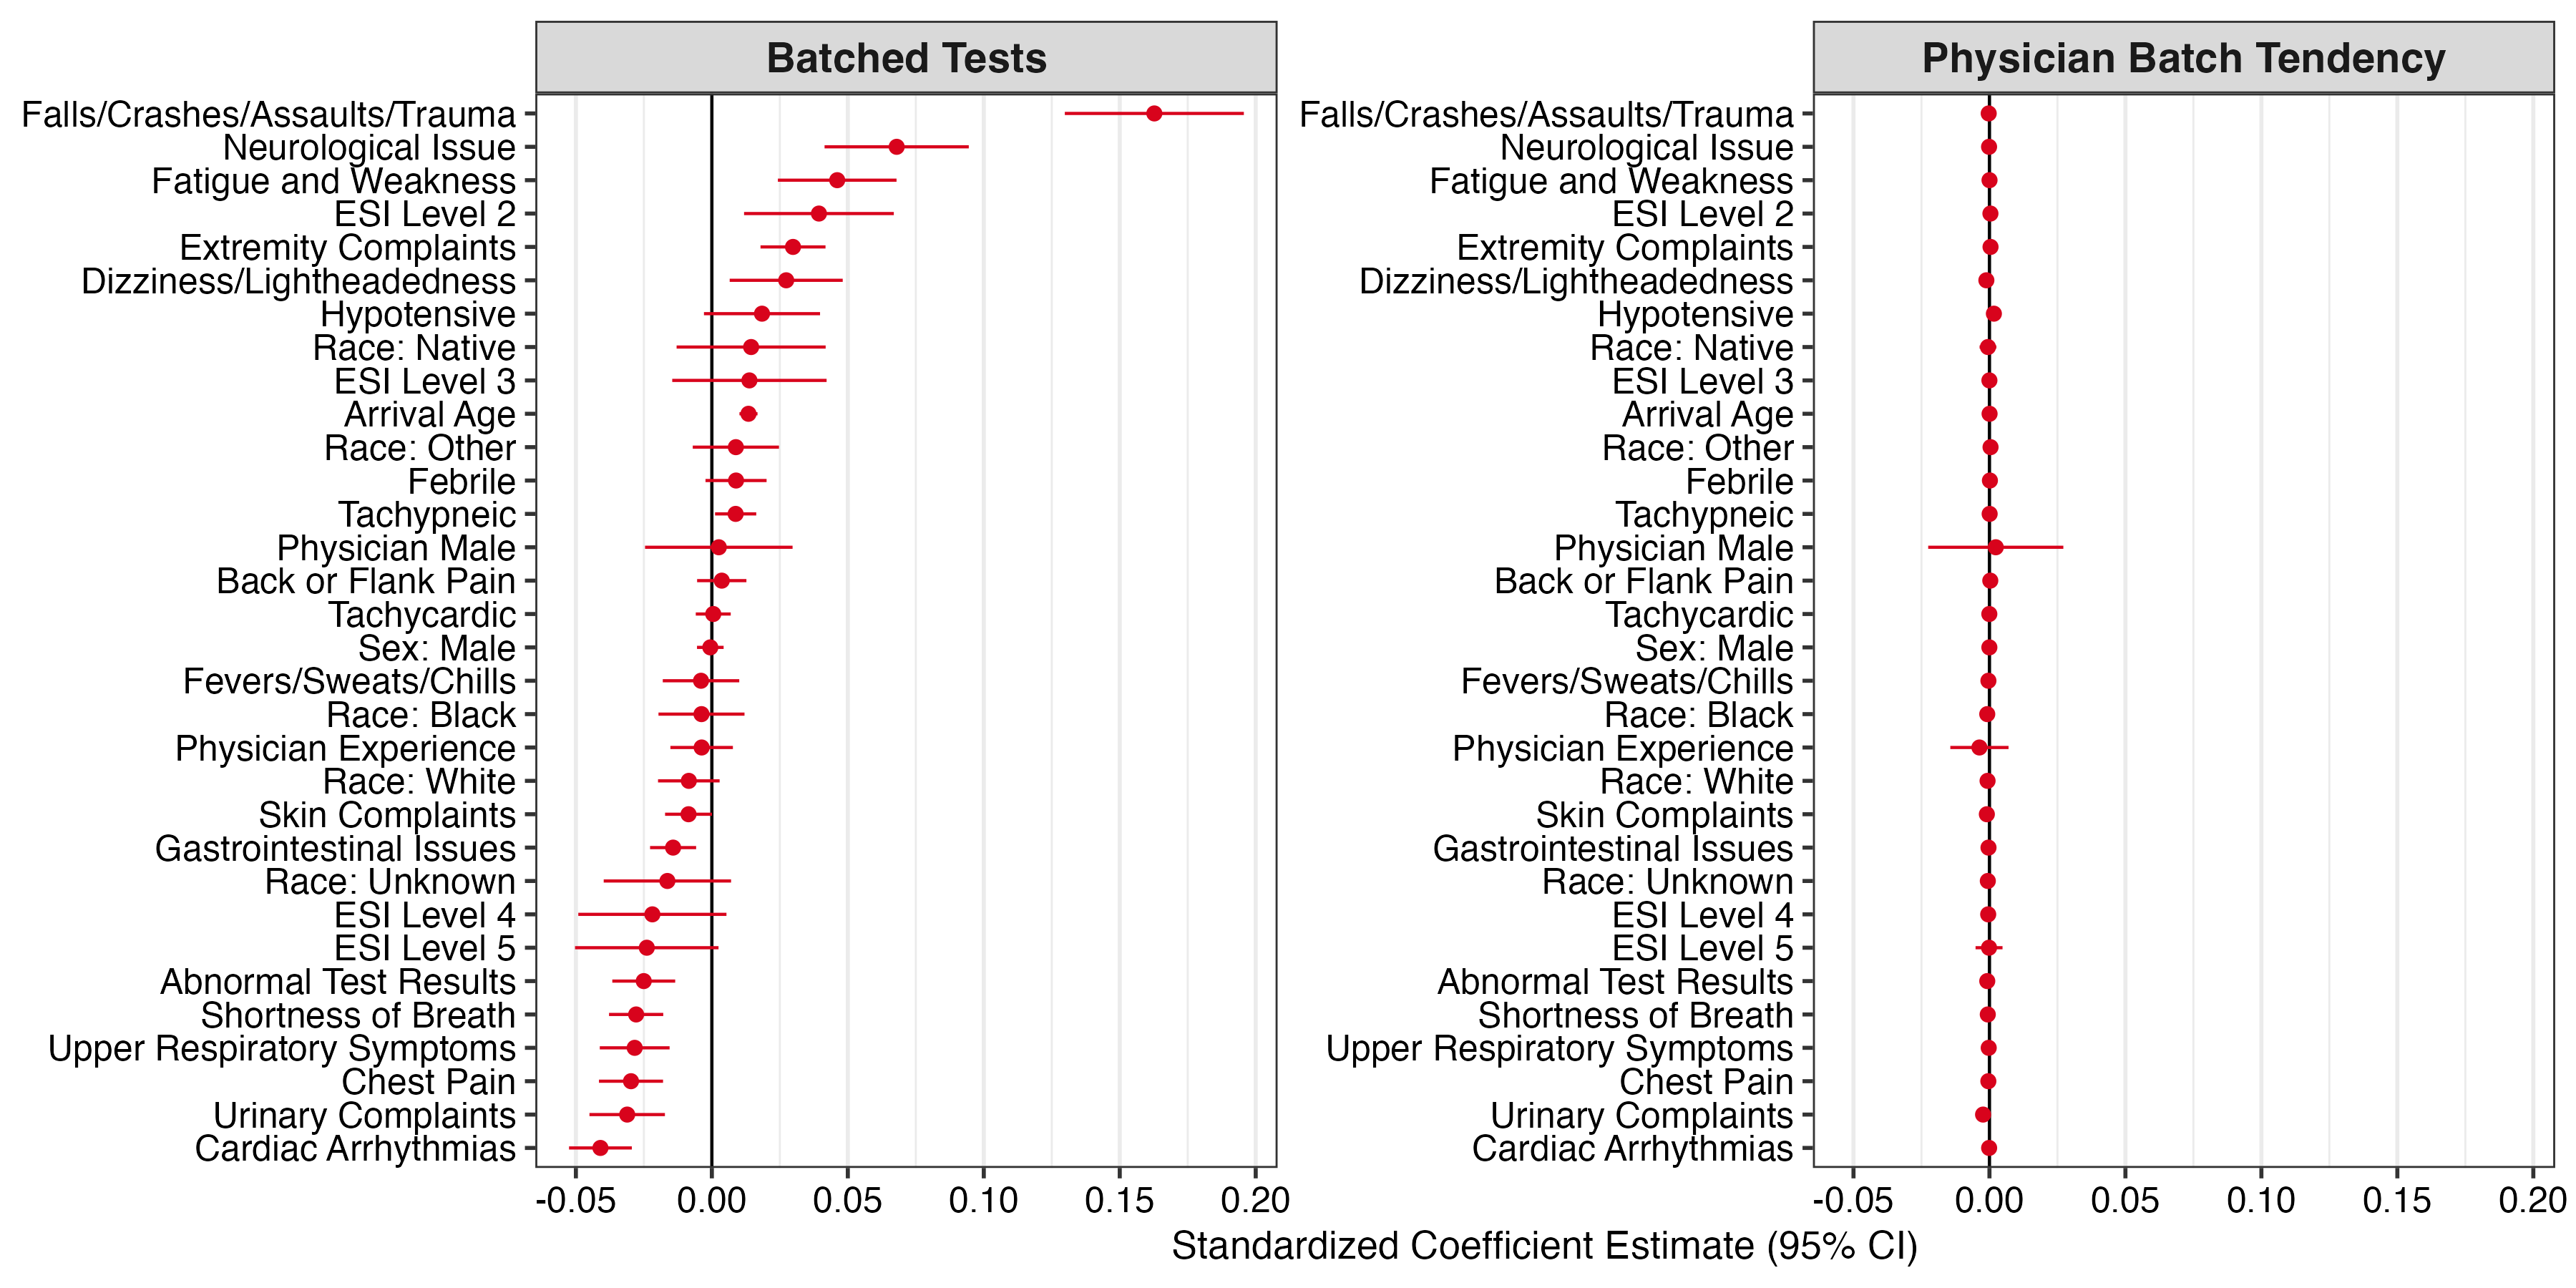
\includegraphics[width=\textwidth]{../outputs/figures/fig2_panel_batched_standardized.png}
    \begin{tablenotes}
        \small
        \item \textit{Notes:} This figure plots a test for quasi-random assignment of patients to physicians in the Mayo Clinic ED. The left panel shows how patient characteristics predict batching decisions. The right panel shows these same characteristics do not predict assignment to physicians with different batch tendencies. Residualization fixed effects include hospital-year-month, hospital-day of week-time of day. Robust standard errors are clustered at the physician level.
    \end{tablenotes}
\end{threeparttable}
\end{figure}

Second, our Local Average Treatment Effect identifies effects for "compliers"—patients whose testing strategy depends on physician assignment rather than clinical protocols. These patients, by definition, represent the discretionary margin where physician preference determines the approach. Our complier analysis in Appendix B reveals approximately 13\% of patients fall into this category—lacking clear clinical indicators mandating either batching or non-batching.

\textbf{2. Are tests medically necessary or preemptively ordered?}

The existence of substantial complier variation—where identical patients receive different testing strategies based on physician assignment—provides definitive evidence of discretionary ordering. If all batching were medically necessary, physician-induced variation would be minimal.

The operational consequences clarify the discretionary nature: for these marginal patients, batching generates 1.2 additional imaging tests (91\% increase, p<0.001) without improving quality outcomes (72-hour return rates: -0.012, p=0.65). While we cannot determine whether specific individual tests are clinically unnecessary, the pattern is clear: at the margin where physicians exercise discretion, batching increases resource utilization without measurable clinical benefits.

Moreover, our heterogeneity analysis (Figure 4) suggested by Reviewer 3 reveals consistent patterns across complaint types. Even for Falls/Trauma/MVA—our most complex category, where comprehensive imaging might seem most justified—discretionary batching still generates additional tests (1.12 tests, p<0.001) without time savings or quality improvements. This suggests that even when physicians anticipate needing multiple tests, preemptive batching still produces operational inefficiencies compared to sequential information-gathering.

\begin{figure}[h]
\centering
\caption*{Figure 4  Heterogeneity in Batch Ordering Effects by Chief Complaint}
\begin{threeparttable}
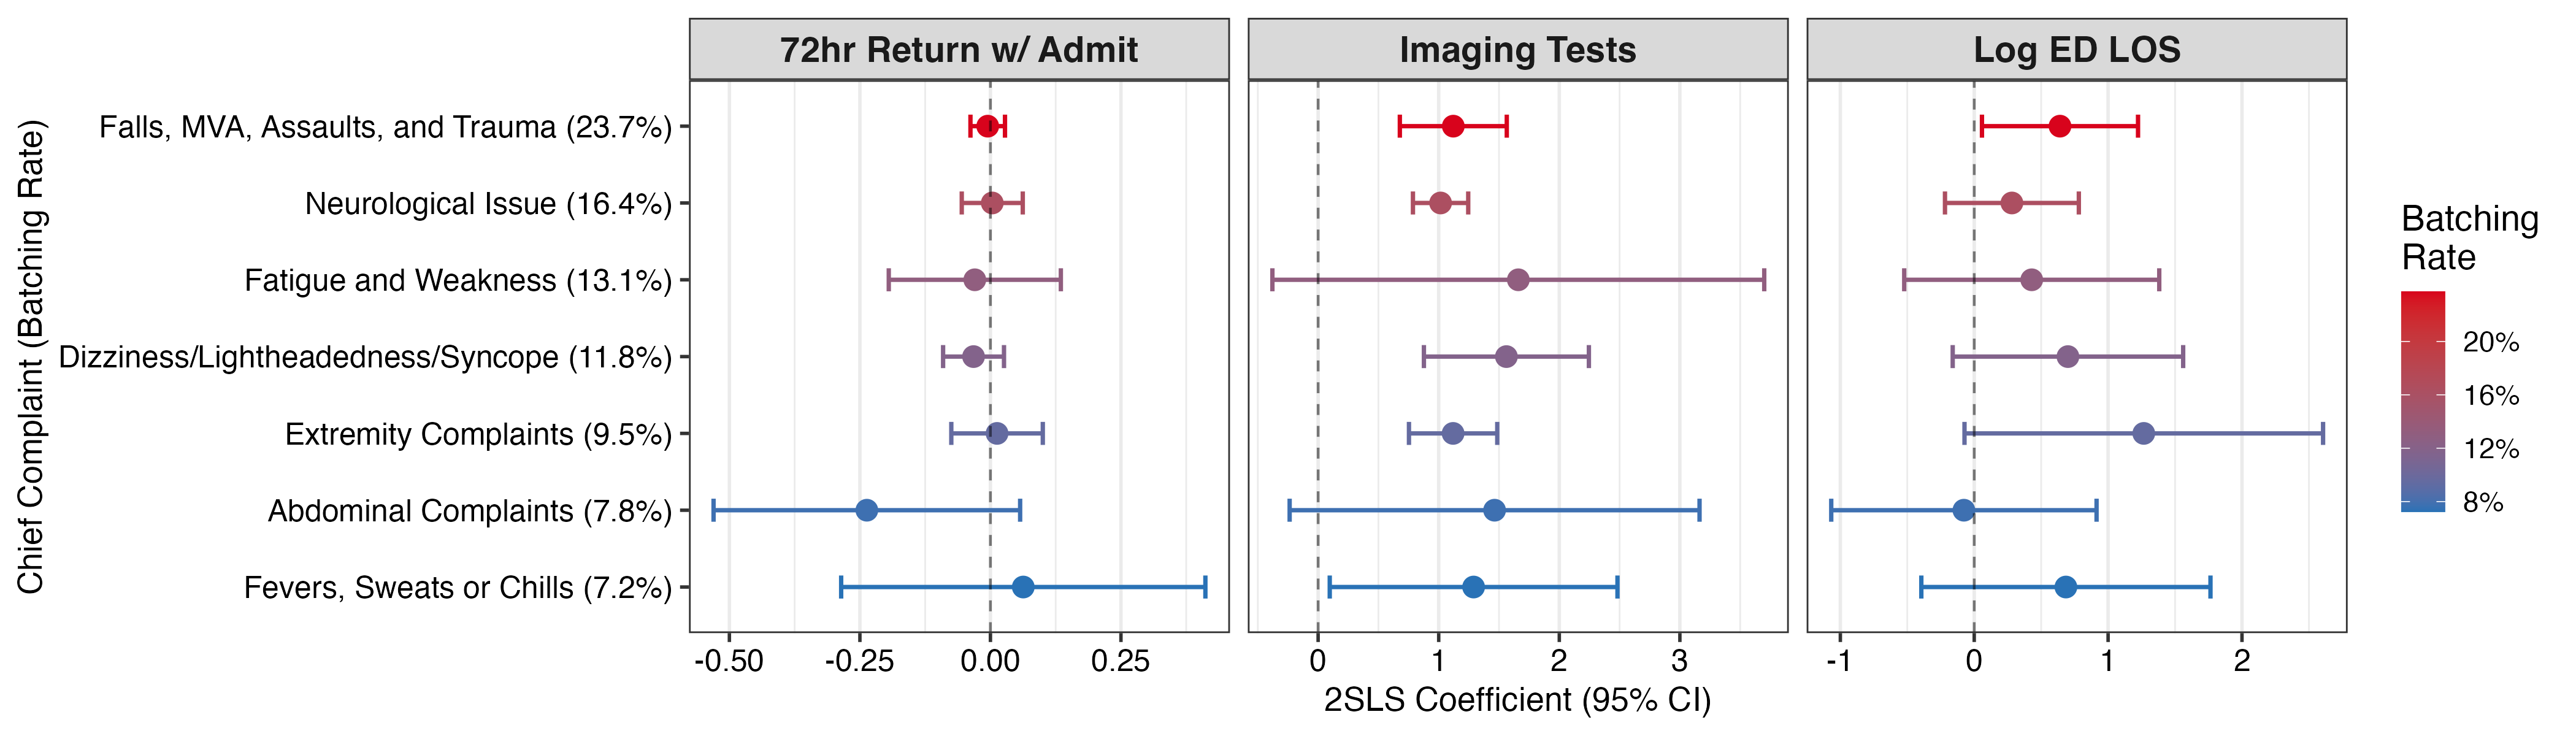
\includegraphics[width=\textwidth]{../outputs/figures/heterogeneity_by_complaint.png}    
\begin{tablenotes}
\small
\item \textit{Notes:} Each panel shows 2SLS estimates of batching effects for different chief complaints, ordered by batching rate (shown in parentheses). Point colors indicate batching prevalence. Error bars show 95\% confidence intervals with standard errors clustered at the physician level. All models include full controls.
\end{tablenotes}
\end{threeparttable}
\end{figure}

\textbf{3. Could batching be a consequence of diagnostic uncertainty or contextual factors?}

We address each potential confound directly:

Our focus on early batching (within 5 minutes of encounter initiation) rules out pending results as a driver. At this point, no prior tests have returned results. Late adaptive batching in response to test results occurs in only 1.9\% of multi-test encounters, confirming that pending results do not drive the batching decisions we study.

If batching were driven by standardized referral protocols (e.g., all trauma patients require specific imaging for specialist consultation), we would observe minimal physician-induced variation—all physicians would batch the same patients. Instead, our complier analysis reveals 13\% of patients receive different testing strategies based solely on physician assignment. Moreover, Mayo Clinic's random assignment mechanism ensures referral requirements are balanced across physicians, so systematic differences in batching rates reflect physician discretion rather than patient-driven protocols.

The random assignment mechanism directly addresses whether uncertain cases drive batching. If diagnostically uncertain patients systematically received more batching, we would observe that patient characteristics predict assignment to high-batching physicians. Figure 2 (right panel) shows this is not the case—patient characteristics do not predict batch tendency, confirming that physician practice style, not case complexity, drives the variation we exploit.

We directly examine whether contextual factors like ED capacity drive batching decisions. However, as Reviewer 3 correctly noted, our capacity-stratified analysis (previously Table 5) does not show statistically significant differences across capacity levels. We have removed claims about capacity heterogeneity and instead note that batching occurs across all operational contexts, with consistent operational inefficiencies (increased imaging without time savings) regardless of ED utilization levels.

\textbf{Manuscript changes:}

We have substantially revised Sections 2.3 (Hypothesis Development) and 3.3 (Identification Strategy) to clarify these theoretical foundations, emphasizing:

\begin{enumerate}
\item The distinction between clinically-necessary and discretionary batching
\item Our LATE targets the discretionary margin where ED interventions can improve efficiency
\item The role of enhanced controls in validating that we capture imaging-specific workflow decisions
\item Interpretation of complier effects and what they reveal about physician decision-making
\end{enumerate}

We appreciate the Associate Editor's guidance, which has enabled us to provide a much clearer theoretical foundation and demonstrate that our enhanced empirical specification directly addresses concerns about whether we truly isolate discretionary behavior.
\color{black}

%%%%%%%%%%%%%%%%%%%%%%%%%%%  AE Comment 3  %%%%%%%%%%%%%%%%%%%%%%%%%%%%%%%%%%
\begin{quote2}
\textbf{AE Wrote (Comment – Empirical concerns):} 

\noindent``The observed effect with an increase of 130\% in ED stay as a result of batching is striking and, in fact, lacks credibility. Such a large effect increases the likelihood of confounding and therefore demands a very high degree of confidence in the empirical approach. As pointed out by several reviewers, there are unresolved concerns regarding the physician-patient assignment process. It is unclear whether this assignment is truly exogenous. For example, some physicians might only work certain shifts or treat specific patient types.

All reviewers were critical of the empirical strategy. Nevertheless, I believe the data offer enough potential to address these concerns through a substantial revision. This would require a significant improvement of both the theoretical development and the empirical analysis.

Based on the reviewers’ feedback and my own assessment, I believe there is a potential path toward eventual publication albeit at a very high risk. In addition to responding to the referee’s concerns, the revision needs to address the following key points:” 
\end{quote2}

\noindent\textbf{Response:} \color{blue}We appreciate the Associate Editor's candid assessment, which precisely identified the central challenges. Our revised analysis directly addresses both concerns raised.

\textbf{1. Effect magnitude and confounding:}

The Associate Editor is correct that the 130\% effect could be due in part to violations of the exclusion restriction. In response to all three reviewers' concerns about confounding, we substantially expanded our control set to ensure our instrument captured imaging-specific behavior rather than general diagnostic intensity. Our revised primary specification (Table 4, Column 5) now controls for:

\begin{itemize}
\item Patient characteristics (vital signs, age, demographics, complaint severity)
\item Physician characteristics (experience, gender, hours into shift)  
\item Realized diagnostic intensity (laboratory tests ordered)
\item Contextual factors (ED capacity, temporal fixed effects)
\end{itemize}

This enhancement directly addresses the confounding concern. Our revised estimates show:

\begin{itemize}
\item Log ED LOS: 0.580 (SE=0.341, p=0.089)
\item Imaging tests: 1.214 (SE=0.196, p<0.001)
\item Admission: 0.392 (SE=0.071, p<0.001)
\end{itemize}

The attenuation of time effects confirms the Associate Editor's intuition about confounding. Our original specification partially captured general diagnostic intensity. However, the persistence of large imaging effects after comprehensive controls demonstrates that substantial imaging-specific variation remains, which is the parameter relevant for ED protocols.

\textbf{2. Assignment process and exogeneity:}

Reviewer 1 raised identical concerns about whether the assignment is truly exogenous. We have substantially expanded Section 3.1 with detailed documentation of Mayo Clinic's rotational system, which addresses the specific scenarios the Associate Editor mentions:

Mayo Clinic employs a computerized rotational assignment algorithm that assigns patients 60 seconds after registration based solely on arrival time. The system does not consider patient demographics, chief complaint, ESI score, physician workload, or recently assigned patient acuity. At shift start, each physician receives four consecutive patients, then enters rotation with other on-duty physicians. The rotation order varies across shifts to prevent systematic advantages.

This design directly addresses the Associate Editor's concerns:

\begin{itemize}
\item Physicians work varying shift times, but temporal fixed effects control for time-of-day patterns
\item Patients cannot be steered to specific physicians based on characteristics
\item Figure 2 provides empirical verification: patient characteristics do not predict assignment to high versus low batch-tendency physicians (all coefficients near zero with confidence intervals crossing zero)
\end{itemize}

We have also implemented an alternative instrument using physician fixed effects (suggested by Reviewer 3), which yields virtually identical results (imaging: 1.219*** vs 1.214***, LOS: 0.571 vs 0.580), providing additional confidence in our identification strategy.

These revisions substantially strengthen confidence in our empirical approach while providing more credible effect magnitudes.
\color{black}


\begin{quote2}
\textbf{AE Wrote (Comment – Hypothesis development):} 
\noindent``The current framing does not clearly distinguish between "batching" and "sequencing" of diagnostic tests. A more precise hypothesis is needed. See also Ref 2 and Ref 3."
\end{quote2}

\noindent\textbf{Response:} \color{blue}The Associate Editor is correct, and Reviewers 1 and 2 raised this identical concern. We have reframed our comparison throughout the manuscript as "batch ordering versus standard practice" rather than "batching versus sequencing."

This clarification addresses the conceptual issue: our counterfactual includes both sequential multi-test encounters and single-test encounters, not pure sequential testing. As we noted in our response to Reviewer 1, this reflects the fundamental information problem physicians face—they cannot know ex-ante which patients will ultimately need multiple tests. Our comparison captures the policy-relevant decision: should physicians commit to comprehensive imaging upfront or preserve diagnostic flexibility?

We have made extensive revisions:

\textbf{Section 2.3 (Hypothesis Development):} Now explicitly frames hypotheses around "batch ordering versus standard practice," clarifying that standard practice preserves the option value of information from initial tests.

\textbf{Section 3.3 (Identification):} Added text clarifying: "Our LATE compares batch ordering to standard practice, which includes both sequential ordering and single tests. While this involves a composite counterfactual, it provides the policy-relevant parameter: the effect of encouraging comprehensive upfront testing versus allowing diagnostic information to guide testing decisions."

\textbf{Abstract and Introduction:} Consistently use "batch ordering versus standard practice" and emphasize that the LATE identifies effects for patients at the margin of clinical discretion.

We hope that this reframing directly addresses the Reviewer and Associate Editor's concern about precision while maintaining an honest interpretation of what our empirical design identifies.

\begin{quote2}
\textbf{AE Wrote (Comment – Outcome variable):} 

\noindent``Consider integrating intermediate outcomes / mechanisms, such as the order and type of tests performed. Are all tests necessary in each case? ED length of stay is a problematic outcome due to factors like patient heterogeneity, workload fluctuations, and staffing variability. The reviewer comments offer several suggestions here.” 

\end{quote2}

\noindent\textbf{Response:} \color{blue}We have substantially enhanced our analysis to address each concern the Associate Editor raises.

Regarding intermediate outcomes and mechanisms, Reviewer 3 raised concerns about reverse causality in Panel B of Table 4, which examines specific test types. We clarified that our IV approach—instrumenting batching with physician tendency calculated from other patients—breaks the endogeneity between patient-specific test needs and batching decisions. The results reveal that discretionary batching nearly universally adds X-rays (97pp increase, p<0.01), while having more minor, non-significant effects on other forms of imaging. This pattern indicates physicians construct comprehensive workups by adding quick, low-cost tests rather than selectively ordering expensive imaging.

Reviewer 2 raised the identical question about whether additional tests represent overuse or appropriate care. While we cannot determine whether specific individual tests are clinically unnecessary, our complier analysis provides definitive evidence of discretionary ordering: 13\% of patients receive different testing strategies based solely on physician assignment. For these marginal patients, batching generates 1.2 additional imaging tests (91\% increase, p<0.001) without improving quality outcomes (72-hour returns: -0.012, p=0.65). This pattern—increased resource utilization without measurable clinical benefits—suggests that at the margin where physicians exercise discretion, additional tests do not provide commensurate value.

The Associate Editor correctly notes that ED LOS captures multiple processes beyond physician decision-making. Following Reviewer 3's suggestion, we added treatment time (time from physician assessment to disposition) as an alternative outcome that excludes both waiting room delays and post-disposition boarding. The results (Appendix D) show nearly identical patterns: 94\% increase (p=0.17) for treatment time versus 88\% increase (p=0.17) for time to disposition. This consistency demonstrates that batching affects clinical processing time, not just mechanical delays.

Our enhanced specification directly addresses the factors the Associate Editor identifies as problematic. For patient heterogeneity, we control for vital signs, age, demographics, chief complaint severity, ESI level, and laboratory testing—comprehensive controls for case mix, with Figure 2 confirming these characteristics do not predict assignment to different physician types. For workload fluctuations, we include ED capacity level indicators (normal, minor overcapacity, major overcapacity) and comprehensive temporal fixed effects (day-of-week × time-of-day, month-of-year) to account for systematic demand patterns. For staffing variability, we control for physician experience, gender, and hours into shift to capture systematic differences in practice patterns and potential fatigue effects.

The robustness of imaging effects (1.214 tests, p<0.001) across these comprehensive controls provides confidence that we capture genuine physician practice variation rather than confounding from operational factors. Together, these enhancements—test-type mechanisms, multiple time measures, and comprehensive controls—address the Associate Editor's concerns about outcome measurement while providing convergent evidence that discretionary batching increases resource utilization without improving efficiency or quality.
\color{black}

\begin{quote2}
\textbf{AE Wrote (Comment – Relevance):} 

\begin{itemize}
    \item ``Focusing on subsets of patients or refining outcomes may help understand and explain the large effect size."
    \item ``A counterfactual cost-benefit analysis could strengthen the case for the practical relevance of the findings.” 
\end{itemize}

\end{quote2}

\noindent\textbf{Response:} \color{blue}We have addressed both suggestions to strengthen the practical relevance of our findings.

Regarding patient subsets and refined outcomes, our revisions directly explain the initially reported large effect size. First, our enhanced control set (adding laboratory ordering, physician characteristics, and hours into shift) reveals that the original 130\% LOS increase was partially driven by general diagnostic intensity rather than imaging-specific batching behavior. Our revised estimate of 79\% (p=0.089) provides a more accurate and credible magnitude, though we acknowledge the effect remains imprecisely estimated.

Second, following Reviewer 3's suggestion, we conducted a heterogeneity analysis across seven chief complaint categories, which vary in clinical complexity and batching prevalence (Figure 4). This exploratory analysis reveals consistent patterns—increased imaging without time savings or quality improvements—across all complaint types, from simple presentations (fevers, extremity complaints) to complex polytrauma cases. The consistency across subgroups strengthens confidence in our main findings while demonstrating that effects do not depend on specific patient populations.

Third, we refined our time-based outcomes by adding treatment time (Reviewer 3's suggestion), which excludes both waiting room delays and post-disposition boarding to isolate physician processing time. The similar patterns across time to disposition (88\% increase) and treatment time (94\% increase) confirm that batching affects clinical decision-making processes, not just mechanical delays. We also compared excluded versus included encounters (Reviewer 3's request), demonstrating that our analytical sample appropriately focuses on moderate-to-high acuity patients where imaging decisions are both consequential and discretionary.

Regarding cost-benefit analysis, Reviewer 2 made this identical suggestion. [NOTE FOR SOROUSH: I am currently in the process of wrapping this comment up for R2. You will notice it is the only one I still need to answer.]

These enhancements—explaining the effect magnitude through enhanced controls, demonstrating consistency across patient subsets, refining outcome measures, and developing cost-benefit implications—substantially strengthen the practical relevance of our findings for ED management.
\color{black}

\begin{quote2}
\textbf{AE Wrote (Comment – Additional suggestions):} 

\noindent``The following additional detailed suggestions could help the authors for developing the manuscript:

\begin{enumerate}
    \item Reassess the definition of the treatment variable (e.g. Ref 3).
    \item Examine the independence of test orders from prior tests and workload conditions (e.g. Ref 2).
    \item Include a section discussing sample representativeness.
    \item Expand the empirical strategy to address unobserved physician and non-physician factors. For instance, Ref 1 recommends using physician fixed effects. Also, reconsider model selection in light of the main outcome.
    \item Re-evaluate whether ED length of stay should remain the primary outcome. Alternative metrics such as time from test order to result may offer more insight."
\end{enumerate}

\end{quote2}

\noindent\textbf{Response:} \color{blue}We have addressed each of these suggestions through substantial revisions responding to the three reviewers.

\textbf{1. Definition of the treatment variable}

Reviewers 1 and 2 raised identical concerns that our comparison was not pure "batching versus sequencing." We have reframed our treatment throughout the manuscript as "batch ordering versus standard practice" and clarified that our counterfactual includes both sequential multi-test encounters and single-test encounters. Section 3.3 now explicitly explains that this composite counterfactual reflects the policy-relevant parameter: the effect of encouraging comprehensive upfront testing versus allowing diagnostic information to guide testing decisions for patients at the margin of clinical discretion—those whose testing strategy is not dictated by apparent clinical necessity but rather depends on physician practice style and judgment. This reframing directly addresses Reviewer 3's concerns about treatment definition precision.

\textbf{2. Independence from prior tests and workload}

Reviewer 2 raised this concern. Our focus on early batching (within 5 minutes of encounter initiation) ensures that no prior test results have returned, ruling out adaptive responses. We document that late batching following initial tests occurs in only 1.9\% of multi-test encounters. For workload conditions, our enhanced specification includes ED capacity level indicators (normal, minor overcapacity, major overcapacity) and comprehensive temporal fixed effects. Additionally, our control for laboratory test ordering directly tests whether imaging decisions are independent of general diagnostic intensity—the persistence of imaging effects (1.214 tests, p<0.001) after this control demonstrates imaging-specific variation.

\textbf{3. Sample representativeness}

Third, Reviewer 3 explicitly requested analysis of sample representativeness. We have added a detailed CONSORT flow diagram (Appendix Figure A2) showing exact exclusion counts at each step and a comprehensive comparison table of excluded versus included encounters (Appendix Table A). The comparison reveals that our analytical sample appropriately focuses on higher-acuity patients presenting with complaints requiring imaging—precisely the population where batching decisions have operational consequences. Section 3.2 now includes an expanded discussion of why this focused sample strengthens rather than limits our contribution.

\textbf{4. Physician fixed effects and model selection}

Reviewer 3 suggested constructing an alternative instrument using physician fixed effects, which we implemented. Appendix D presents results using leave-one-out corrected physician fixed effects as the instrument, yielding virtually identical estimates (imaging: 1.219*** vs 1.214***, LOS: 0.571 vs 0.580). This robustness check validates our main approach. Reviewer 3 also questioned our use of linear models for binary and count outcomes. We have added to Appendix D, which shows that OLS estimates using logit (for binary outcomes) and negative binomial (for count outcomes) yield similar average marginal effects, confirming that functional form does not drive our results. We retain linear 2SLS throughout because nonlinear IV specifications create fundamental econometric problems (the "forbidden regression"), as documented in our response to Reviewer 3.

\textbf{4. Alternative outcomes}

Reviewer 3 suggested treatment time as an alternative to ED LOS that excludes waiting room delays and post-disposition boarding. We have added this measure (Appendix D), which shows consistent patterns: a 94\% increase in treatment time, an 88\% increase in time to disposition, and a 79\% increase in total LOS. The consistency across multiple time measures—all capturing different aspects of operational flow—strengthens confidence in our findings. We maintain multiple time-based outcomes in Table 4 rather than selecting a single primary metric, as each captures different policy-relevant aspects of ED efficiency.

These revisions—clarifying treatment definition, establishing test order independence, documenting sample representativeness, implementing alternative empirical specifications, and expanding outcome measures—directly address all five suggestions while maintaining consistency with the three reviewers' detailed feedback.
\color{black}


%%%%%%%%%%%%%%%%%%%%%%%%%%%%%%%%%%%%%%%%%%%%%%%%%%%%%%%%%%%%%%%%%%%%%%%%%%%%%%
% End of AE responses
%%%%%%%%%%%%%%%%%%%%%%%%%%%%%%%%%%%%%%%%%%%%%%%%%%%%%%%%%%%%%%%%%%%%%%%%%%%%%%

\clearpage

%%%%%%%%%%%%%%%%%%%%%%%%%%%%%%%%%%%%%%%%%%%%%%%%%%%%%%%%%%%%%%%%%%%%%%%%%%%%%%
%%  SECTION IV – RESPONSES TO REVIEWER 1 COMMENTS                           %%
%%%%%%%%%%%%%%%%%%%%%%%%%%%%%%%%%%%%%%%%%%%%%%%%%%%%%%%%%%%%%%%%%%%%%%%%%%%%%%

\pagestyle{fancy}
\fancyhead{}
\fancyhead[RO]{\small{Responses to Referee 1 Comments}}
\renewcommand{\headrulewidth}{0pt}

\noindent\underline{\textbf{III. Responses to Referee 1 (R1) Comments}}

%%%%%%%%%%%%%%%%%%%%%%%%%%%  R1 Comment 1  %%%%%%%%%%%%%%%%%%%%%%%%%%%%%%%%%%
\begin{quote2}
\textbf{R1 Wrote (Research question \& contribution):}  

\noindent``The research question is clear, and it is an important area of study. Emergency departments are
high-stress work environments where the stakes are high and patient lives are at stake.
Anything we can learn to improve the performance and outcomes of the work that is done there
could save lives, and also enhance our understanding of the impact of “work behavior /
preferences” on operational outcomes.” 
\end{quote2}

\noindent\textbf{Response:} \textcolor{blue}{We sincerely appreciate the reviewer's recognition of the importance and clarity of our research question. Emergency departments represent uniquely high-stakes environments where operational improvements can have significant implications for patient care. We share the reviewer's view that understanding how physician work behavior affects operational outcomes can bridge individual decision-making and system-level performance. We have strengthened our analysis in response to the methodological concerns raised, and believe the revisions substantially improve the manuscript's rigor and contribution.}

\begin{quote2}
\textbf{R1 Wrote (Major Concern 1):}  

\noindent``The authors apply an interesting method from economics to exploit a setting where patients are assigned to physicians in a random fashion. While this is a nice idea, I have two major concerns about the implementation of the methods in this paper. First, it is unclear to me whether the main explanatory variable is actually testing the main hypothesis presented in the paper, and second, the exclusion restriction assumption (required for an IV to be valid in presenting causal
estimates) is not met.


\noindent On On page 4 of the manuscript (Section 1.2 – Main Findings and Contributions), the authors state “our results show that the marginal batched patient experiences a 130\% increase in total ED LOS and an 123\% increase in time to disposition compared to patients who have their tests ordered sequentially”. It is not clear to me that you are in fact testing the effect of batching compared to sequential test ordering. Here, the main explanatory variable is Batched, which is defined as a binary variable that equals 1 if the physician ordered 2 or more imaging tests of different modalities within a five-minute window at the start of the patient’s visit and 0 otherwise. This otherwise, acting as a counterfactual baseline, covers not only cases where the physician is ordering the same number of tests sequentially. It also covers cases where the physician orders fewer tests, or none at all. As such, the Batched variable is actually modeling some element of physician practice style like “degree of cautiousness” or “affinity for comprehensive testing”. So, it is unsurprising that patients exposed to high-“batch tendency” physicians also have higher testing volumes and higher LOS – if a physician has a tendency to order more imaging, they may also have a tendency to order more labs or be more comprehensive in other ways that are not observed in the data.

If you are interested in studying the impact of batching imaging orders versus sequentially ordering them, as is currently discussed in the paper, then perhaps consider matching patients who have similar conditions and who we know ultimately have the same number of tests ordered – one patient would have had the orders batched, and the other would have them ordered sequentially. Though, I imagine doing something like this would result in limitations with respect to sample size, similar issues as in the current design where fewer tests are ordered when done sequentially (especially if the patient ends up being admitted and getting these tests when they are on an inpatient unit), among other endogeneity concerns.

Regardless, in its current manifestation, the batched variable is not capturing physician batching compared to sequential testing, and many of the managerial implications and conclusions currently presented in the paper do not logically follow from the presented results."
\end{quote2}

\noindent\textbf{Response:} \color{blue}We thank the reviewer for this thoughtful critique, which has led to substantial improvements in how we frame our research question and interpret our results. The reviewer raises two key concerns: (1) our counterfactual includes heterogeneous cases, and (2) our instrument might capture general physician cautiousness rather than batching behavior specifically. We address each in turn.

\textbf{1. Clarifying the counterfactual}: First, an essential clarification: our sample includes only encounters where at least one imaging test was ordered. The $Batched=0$ group, therefore, comprises patients who received either (1) a single imaging test, or (2) multiple tests ordered sequentially—but not patients with zero imaging. This distinction is critical because our comparison is between different imaging strategies for patients who require diagnostic imaging, not between testing and no testing.

That said, the reviewer correctly identifies that our counterfactual remains composite—mixing single-test and sequential multi-test encounters. The reviewer suggests matching patients on eventual test count but correctly anticipates the key limitation: this would introduce severe post-treatment bias since batching causally affects subsequent testing decisions. Physicians cannot know ex ante which patients will ultimately require multiple tests—they make batching decisions under diagnostic uncertainty. Conditioning on the eventual test count would compare fundamentally different populations after the treatment has already occurred. Furthermore, matching would estimate the Average Treatment Effect on the Treated (ATT)---comparing patients who received batching to observably similar patients who did not. The ATT conflates effects across all patients, including always-takers (where batching is clinically mandated) and never-takers (where single tests suffice). This parameter has limited managerial relevance since ED protocols cannot change testing patterns where clinical necessity dictates the approach.

Our IV approach preserves causal interpretation by identifying effects at the moment of decision-making. The LATE captures effects for ``compliers"—patients whose testing strategy depends on physician assignment rather than clinical necessity. These marginal patients represent precisely where ED protocols can influence practice without constraining clinically necessary care.

In response to this feedback, we have reframed our comparison throughout the manuscript as ``batch ordering versus standard practice." This standard practice encompasses both sequential ordering and single-test cases among patients who receive at least one imaging test. The terminology change clarifies that we compare a discretionary practice pattern (early comprehensive imaging) against the standard approach (preserving diagnostic flexibility). We added text in Section 3.3 clarifying:

\begin{quote}
``Our two-stage least squares estimates represent the LATE of batch ordering for `compliers'---patients whose testing strategy depends on the assigned physician's practice style. This effect compares batch ordering to standard practice, which includes both sequential ordering and single tests. While this involves a composite counterfactual, it provides the policy-relevant parameter: the effect of encouraging comprehensive upfront testing versus allowing diagnostic information to guide testing decisions for patients at the margin of clinical discretion—those whose testing strategy is not dictated by apparent clinical necessity but rather depends on physician practice style and judgment."
\end{quote}

This framing reflects the fundamental information structure of emergency medicine. At the time of initial ordering, physicians cannot know which patients will ultimately need multiple tests versus a single test. They must decide whether to commit to comprehensive imaging upfront or preserve diagnostic flexibility. We have added a discussion of this information problem in Section 3.2.1:

\begin{quote}
``We focus on batches that concern the first imaging tests ordered during the patient encounter because this represents the moment of maximum diagnostic uncertainty, when physicians must decide their testing strategy before clinical information unfolds. Physicians cannot know ex-ante which patients will ultimately require multiple tests, leading to instances in which batching is a discretionary choice based on practice style rather than clinical necessity."
\end{quote}

We also clarified the policy relevance of this comparison in Section 5.1:

\begin{quote}
``This comparison reflects the real choice facing ED managers: should protocols encourage comprehensive upfront testing or preserve diagnostic flexibility? Our estimates show that preserving optionality through standard practice---which allows information from initial tests to guide subsequent decisions---reduces testing intensity."
\end{quote}

\textbf{2. Addressing the exclusion restriction concern through expanded controls:}

The reviewer's concern—that our instrument might capture general ``comprehensiveness" rather than batching-specific behavior—is exactly right to scrutinize. The reviewer notes that if a physician has a tendency to order more imaging, they may also tend to order more labs or be more comprehensive in other ways. This is a valid concern that we take seriously.

In our original specification, we controlled only for patient characteristics (vital signs, age, demographics, chief complaint severity) and temporal factors (shift-level effects). In response to concerns from all three reviewers, we have substantially expanded our control set to test whether batch tendency reflects general diagnostic intensity versus imaging-specific timing decisions.

Our revised primary specification now includes:

\begin{itemize}
\item \textbf{Patient characteristics:} Vital signs (tachycardic, tachypneic, febrile, hypotensive), age, demographics, chief complaint severity
\item \textbf{Physician characteristics:} Years of experience, gender, hours into shift (capturing potential fatigue effects)
\item \textbf{Realized diagnostic intensity:} Indicator for whether laboratory tests were performed during the encounter
\item \textbf{Contextual factors:} ED capacity level (normal, minor overcapacity, major overcapacity), temporal fixed effects
\end{itemize}

The addition of laboratory test ordering is critical. If batch tendency captures physicians who are generally more aggressive or comprehensive diagnosticians, they should order both more imaging and more labs. By controlling for whether labs were actually ordered for each patient, we test whether imaging effects persist when accounting for the thoroughness of general diagnostics. If batch tendency reflected "comprehensive diagnosticians," controlling for realized lab intensity should substantially attenuate imaging effects.

First-stage results validate the concern while demonstrating that we can isolate the imaging-specific component. Below, we show how the first stage changes as we progressively add these new controls:

\begin{table}[ht]
\centering
\caption*{First-Stage Robustness: Batch Tendency Predicts Batching}
\label{tab:first_stage_robustness}
\begin{threeparttable}
\begin{tabular}{lcccc}
\toprule 
& \multicolumn{4}{c}{Dependent Variable: Batched}\\
\cmidrule(lr){2-5}
& (1) & (2) & (3) & (4) \\
\midrule
Batch Tendency & 2.018*** & 2.026*** & 2.023*** & \textbf{1.911***} \\ 
& (0.090) & (0.090) & (0.090) & \textbf{(0.115)} \\
\midrule
\textit{Controls} \\
Time Fixed Effects & Yes & Yes & Yes & Yes \\
Patient Controls & Yes & Yes & Yes & Yes \\
Physician Exp \& Sex & No & Yes & Yes & Yes \\
Hours into Shift & No & No & Yes & Yes \\
Laboratory Ordered & No & No & No & Yes \\
\midrule
F-statistic & 503.6 & 509.8 & 507.5 & \textbf{276.8} \\
$p$-value & <0.001 & <0.001 & <0.001 & <0.001 \\
Observations & 11,651 & 11,651 & 11,651 & 11,651 \\
\bottomrule
\end{tabular}
\begin{tablenotes}
\footnotesize
\item \textit{Notes:} First-stage regressions of batching on batch.tendency (leave-one-out physician residualized batching propensity). Standard errors clustered at the physician level in parentheses. Patient controls include vital signs, age, demographics, chief complaint-severity fixed effects, race, and gender. All models include day-of-week × time-of-day fixed effects, month fixed effects, and ED capacity controls. *** p<0.001.
\end{tablenotes}
\end{threeparttable}
\end{table}

Three key observations emerge:

1. Physician characteristics have minimal effect on the first stage (F: 503.6 → 509.8). Experience, gender, and hours into shift are essentially orthogonal to batching propensity.

2. Laboratory ordering substantially attenuates the first stage (F: 507.5 → 276.8, coefficient: 2.023 → 1.911). This confirms the reviewer's intuition—batch tendency was partially capturing general diagnostic intensity, exactly as suspected.

3. Substantial independent variation remains (F=276.8, well above weak instrument thresholds). After controlling for general diagnostic thoroughness, significant imaging-specific variation persists. This is precisely what we would expect if the instrument captures imaging timing decisions rather than purely general cautiousness.

The table below (for response letter only) shows how our 2SLS estimates change as we add each control set:

\begin{table}[H]
\centering
\caption*{2SLS Results: Progressive Addition of Controls}
\begin{threeparttable}
\small
\begin{tabular}{lcccc}
\toprule
& (1) & (2) & (3) & (4) \\
\midrule
\multicolumn{4}{l}{\textit{Panel A: Time-Based Outcomes}} \\[0.5em]
Log ED LOS & 0.679** & 0.699** & 0.759**  & 0.580. \\
& (0.341) & (0.331) & (0.342)  & (0.341) \\[0.5em]
Log time to disposition & 0.618 & 0.618 & 0.693 & 0.630 \\
& (0.456) & (0.435) & (0.437)  & (0.460) \\[0.5em]

\multicolumn{4}{l}{\textit{Panel B: Resource Utilization}} \\[0.5em]
Imaging tests & 1.360*** & 1.372*** & 1.316***  & 1.214*** \\
& (0.199) & (0.209) & (0.208) & (0.196) \\[0.5em]

\multicolumn{4}{l}{\textit{Panel C: Patient Outcomes}} \\[0.5em]
72hr return w/ admit & -0.011 & -0.009 & -0.009  & -0.012 \\
& (0.021) & (0.021) & (0.023) & (0.025) \\[0.5em]
Admitted & 0.397*** & 0.427*** & 0.481***  & 0.392*** \\
& (0.088) & (0.105) & (0.083)  & (0.071) \\
\midrule
\textit{Controls} \\
Time Fixed Effects & Yes & Yes & Yes & Yes \\
Patient Controls & Yes & Yes & Yes & Yes \\
Physician Exp \& Sex & No & Yes & Yes & Yes \\
Hours into Shift & No & No & Yes & Yes \\
Laboratory Ordered & No & No & No & Yes \\
\midrule
Observations & 11,651 & 11,651 & 11,651 & 11,651 \\
\bottomrule
\end{tabular}
\begin{tablenotes}
\footnotesize
\item \textit{Notes:} 2SLS estimates with batch tendency as instrument. Standard errors clustered at the physician level. All specifications include temporal fixed effects and chief complaint-severity fixed effects. Patient controls include vital signs and age. Physician controls include experience and gender. 
\item . p<0.10, ** p<0.01, *** p<0.001.
\end{tablenotes}
\end{threeparttable}
\end{table}

Through this experiment, we see that physician characteristics have minimal impact on estimates (comparing columns 1 and 2). This demonstrates that batch tendency is not simply proxying for experience or gender-based practice patterns. We also find that laboratory ordering controls attenuate time effects (comparing columns 3 and 4), confirming that our original specification partially conflated general diagnostic intensity with imaging-specific behavior. However, imaging test volume effects remain large and highly significant (1.214 additional tests, p<0.001), demonstrating that batch tendency retains substantial imaging-specific variation even after controlling for general diagnostic thoroughness.

Our revised main results (Table 4) now appear in the manuscript. Table 4 presents both OLS and 2SLS results; columns 4-5 show 2SLS estimates corresponding to specifications (1) and (4) from the progressive analysis above:

\begin{table}[h]
\centering
\caption*{Table 4     IV Results: Effect of Batching Tests on Patient Outcomes}
\label{tab:results_table}
\begin{threeparttable}
\begin{tabular}{lccccc}
\toprule
& Sequenced & \multicolumn{2}{c}{\underline{OLS results}} & \multicolumn{2}{c}{\underline{2SLS results}} \\
& mean & (2) & (3) & (4) & (5) \\
\midrule
\multicolumn{6}{l}{\textit{Panel A. Primary Outcomes}} \\[0.5em]
Log time to disposition & 5.237 & $0.084^{***}$ & $0.072^{***}$ & $0.618$ & $0.630$ \\
& (0.499) & (0.014) & (0.013) & (0.456) & (0.460) \\[0.5em]
Log LOS & 5.490 & $0.107^{***}$ & $0.073^{***}$ & $0.679^{\dagger}$ & $0.580$ \\
& (0.456) & (0.013) & (0.012) & (0.341) & (0.341) \\[0.5em]
Number of distinct imaging tests & 1.334 & $0.839^{***}$ & $0.802^{***}$ & $1.360^{***}$ & $1.214^{***}$ \\
& (0.571) & (0.017) & (0.019) & (0.199) & (0.196) \\[0.5em]
72hr return with admission & 0.012 & -0.001 & 0.000 & -0.011 & -0.012 \\
& (0.110) & (0.002) & (0.003) & (0.021) & (0.025) \\[0.5em]

\multicolumn{6}{l}{\textit{Panel B. Test Types}} \\[0.5em]
Ultrasound & 0.171 & $0.072^{***}$ & $0.117^{***}$ & 0.162 & 0.089 \\
& (0.376) & (0.016) & (0.014) & (0.101) & (0.082) \\[0.5em]
CT with contrast & 0.187 & 0.029 & $0.051^{**}$ & $0.168^{\dagger}$ & 0.085 \\
& (0.390) & (0.015) & (0.014) & (0.071) & (0.069) \\[0.5em]
CT without contrast & 0.400 & $0.383^{***}$ & $0.279^{***}$ & 0.105 & 0.067 \\
& (0.490) & (0.015) & (0.012) & (0.137) & (0.138) \\[0.5em]
X-ray & 0.576 & $0.354^{***}$ & $0.356^{***}$ & $0.925^{***}$ & $0.972^{**}$ \\
& (0.494) & (0.012) & (0.012) & (0.220) & (0.260) \\[0.5em]

\multicolumn{6}{l}{\textit{Panel C. Disposition}} \\[0.5em]
Admission & 0.279 & $0.035^{*}$ & $0.027^{**}$ & $0.397^{***}$ & $0.392^{***}$ \\
& (0.449) & (0.013) & (0.009) & (0.088) & (0.071) \\[0.5em]
\midrule
Time FE & --- & Yes & Yes & Yes & Yes \\
Baseline controls & --- & No & Yes & No & Yes \\
Observations & 11,651 & 11,651 & 11,651 & 11,651 & 11,651 \\
\bottomrule
\end{tabular}
\begin{tablenotes}
\footnotesize
\item \textit{Notes:} This table reports the estimated coefficients of both OLS and 2SLS regressions of the effect of batching on patient outcomes. The OLS columns include no controls (column 2) and baseline controls (column 3). The 2SLS columns include no controls (column 4) and baseline controls (column 5). Standard errors are clustered at the physician level.
\item $^{\dagger} p < 0.10$, $^{*} p < 0.05$, $^{**} p < 0.01$, $^{***} p < 0.001$.
\end{tablenotes}
\end{threeparttable}
\end{table}

Column 5 represents our primary 2SLS specification with full controls. We acknowledge that these results differ from our original submission, where we reported larger, statistically significant time effects:

\textit{Original submission:}
\begin{itemize}
\item Log LOS: 0.837 (SE=0.299, p=0.005) → 131\% increase
\item Controls: Patient characteristics and temporal factors only
\end{itemize}

\textit{This revision:}
\begin{itemize}
\item Log LOS: 0.580 (SE=0.341, p=0.089) → 79\% increase
\item Controls: Patient + physician + laboratory ordering + hours into shift
\end{itemize}

The attenuation confirms the reviewer's intuition—our original instrument partially captured general diagnostic intensity, not just imaging-specific timing. Our revised specification more precisely isolates the imaging-specific component by controlling for realized laboratory intensity. While time effects lose statistical significance at conventional levels, this reflects a more conservative, defensible specification that addresses the reviewer's core concern.

Despite these changes, our substantive conclusions remain important. We find: (1) batching increases imaging test volume by 91\% (p<0.001), (2) no evidence that batching reduces processing time (point estimates suggest 79-88\% increases, p>0.05), and (3) batching increases admissions by 39 percentage points (p<0.001) with no improvement in 72-hour returns (p=0.65).

This more conservative interpretation directly addresses an active debate among emergency physicians. Some EPs argue that batching is "time-saving" by getting all test orders done upfront. Our evidence refutes this claim—we find no support for time savings, and if anything, point estimates suggest substantial delays. Combined with definitive evidence of increased resource utilization and higher admissions without quality gains, this provides important managerial guidance: discretionary batch ordering is not a time-saving strategy and substantially increases diagnostic intensity.

Combined with balance tests (Figure 2) and null placebo results (Appendix D.1), this provides robust support for our core conclusion. The LATE we estimate represents the effect for compliers—patients whose testing strategy depends on physician practice style rather than clinical necessity. These marginal patients are precisely where ED management interventions (decision support systems, protocols, physician feedback) can influence practice. The finding that batching increases imaging test volume, raises admission rates, and does not improve ED processing times or short-term quality metrics suggests that policies encouraging diagnostic flexibility over comprehensive upfront testing could meaningfully improve ED operational efficiency without harming patient outcomes.

In light of this, we have made several major revisions to the manuscript to enhance clarity and robustness:

\begin{enumerate}
\item \textit{Added comprehensive robustness tables (Appendix D):} We present first-stage, reduced form, and 2SLS results with progressive controls.
\item \textit{Enhanced identification discussion (Section 3.3):} We now explicitly acknowledge that physician tendency instruments may capture bundles of correlated practices. We explain our validation approach through balance tests, placebo tests, and comprehensive controls to isolate imaging-specific effects.
\item \textit{Clarified interpretation of results:} We temper our language throughout the manuscript to reflect the more conservative estimates of our new specification, emphasizing increased resource utilization and lack of evidence for time savings, while acknowledging statistical uncertainty.
\item \textit{Expanded limitations discussion (Section 4.8):} We acknowledge that while we cannot definitively rule out all exclusion restriction violations, the convergence of evidence supports our interpretation. We also discuss the broader context of physician practice style research, noting that while such instruments may capture correlated behaviors, they remain valuable for understanding how discretionary practices impact outcomes. Additionally, our reduced form results do not require the exclusion restriction to represent a causal effect of being assigned a high-batching physician.
\end{enumerate}

We acknowledge important limitations. We cannot definitively rule out all exclusion restriction violations—no observational study can. Despite these limitations, we hope that the reviewer finds that our revisions strengthen our identification strategy while maintaining transparency about the assumptions underlying our causal claims.

\color{black}



%%%%%%%%%%%%%%%%%%%%%%%%%%%  R1 Comment 3  %%%%%%%%%%%%%%%%%%%%%%%%%%%%%%%%%%
\begin{quote2}
\textbf{R1 Wrote (Major Concern 2 – Endogeneity concerns):}  

\noindent ``As discussed by the authors on page 16 of the manuscript, ensuring the exclusion restriction is met to establish valid causal estimates using the proposed instrument is challenging, and not directly testable. However, the authors argue that “such violations may likely only have a small impact and may be less concerning than in other healthcare settings”. This is a requirement to establish causal claims (which the authors claim to want to do), and as outlined in Major Concern 1 above, “high batching tendency” is likely to be correlated by other elements of a physician’s “practice style” that could directly affect the outcomes being tested, outside of only batching imaging. A physician who is more cautious and comprehensive could also order more lab tests, which take time, and thus extend the LOS. A physician who is more cautious and comprehensive could also take longer on the examination, and choose to monitor the patient for a longer period of time before making a disposition decision. Both of these examples could directly impact the outcome without going through imaging batching, thus violating the exclusion restriction. As such, we cannot be certain that the estimates found in this paper are causal estimates on the impact of batching on ED outcomes (even assuming that the main explanatory variable captures batching, which I argue has its own flaw in Major Concern 1).” 
\end{quote2}


\noindent\textbf{Response:} \color{blue}We appreciate the reviewer reiterating this fundamental concern about exclusion restriction violations. As stated in our response to Major Concern 1, we have substantially expanded our controls to test whether batch tendency captures these correlated behaviors and believe that the manuscript, findings, and implications have been strengthened as a result.

We now control for whether labs were ordered for each patient. The reviewer's first example—that high-batch physicians might order more labs, which extend LOS—is directly tested by this control. After controlling for lab ordering, imaging effects remain large and significant (1.214, p<0.001), while time effects show the attenuation the reviewer anticipated. Additionally, we control for physician experience, gender, and hours worked in a shift to capture systematic differences in examination patterns and monitoring decisions.

We acknowledge the reviewer's point that we cannot definitively rule out all exclusion restriction violations. However, we note two important qualifications to this concern:

First, our revised specification directly tests the reviewer's specific examples and finds that while some correlation exists (as evidenced by attenuation of time effects with lab controls), imaging-specific variation persists. The reviewer's concern that we "argue such violations may likely only have a small impact" referred to our original specification. We have removed this language and instead provide empirical evidence through our expanded controls, which show the existence of correlations and demonstrate that substantial imaging-specific effects persist.

Second, even if exclusion restriction concerns persist, our reduced-form estimates—the direct effect of being assigned to a high-batch-tendency physician—represent causal effects of physician assignment that do not require the exclusion restriction. These estimates inform ED management decisions about physician training, feedback, and protocols regardless of the precise mechanism. When we control for observable pathways (labs, physician characteristics), the reduced-form effects remain substantial for imaging volume, while attenuating for time outcomes, providing managers with actionable evidence about which outcomes are most affected by physician assignment.

We have revised Section 4.8 (Limitations) to acknowledge this concern more directly, removing claims that violations "may likely only have a small impact" and instead transparently presenting our validation evidence through expanded controls, while acknowledging that definitive exclusion restriction tests are not possible in observational settings.

\color{black}

%%%%%%%%%%%%%%%%%%%%%%%%%%%  R1 Comment 4  %%%%%%%%%%%%%%%%%%%%%%%%%%%%%%%%%%
\begin{quote2}
\textbf{R1 Wrote (Minor Concern – Randomization mechanism clarity):}  

\noindent``In this report I am taking the authors’ word regarding the randomization of patient to physician matching as described in the paper. More details on this should be given, and the patient-to physician assignment can be empirically shown – if the patients are assigned to physicians in a round-robin format, and you know when patients arrive at the hospital, and which physicians are working, you can empirically show that assignment is random. This is an important part of the empirical design of the paper, and so future iterations should show this empirically. Related to this, there is also the question of what the the queue configuration of the physicians look like – if it is random, and there are 5 physicians working, which physician gets the first patient? Is it by alphabetical order? More detail to describe this assignment mechanism would be helpful.” 
\end{quote2}

\noindent\textbf{Response:} \color{blue}We thank the reviewer for requesting additional detail about the patient-physician assignment mechanism, which is crucial to our identification strategy. We have substantially expanded Section 3.1 with detailed description of Mayo Clinic's rotational assignment system, documented in prior publications at this site \cite{Traub2016, traub2016emergency, Traub2018}. 

The key institutional features address the reviewer's specific questions:

\textbf{Assignment mechanism:} Patients are automatically assigned to physicians 60 seconds after registration through a computerized algorithm in the electronic health record system. Assignment is based solely on arrival time—the algorithm does not consider patient demographics, chief complaint, Emergency Severity Index score, physician workload, or the acuity of recently assigned patients.

\textbf{Rotation initialization and ordering:} At shift start, each physician receives four consecutive patients to establish an initial patient load, after which they enter rotation with other on-duty physicians. The rotation order is predetermined by the ED scheduler and varies across shifts to prevent systematic advantages (e.g., Physician A might be first in Monday morning's rotation but third on Tuesday evening). This scheduling variation ensures no physician systematically receives healthier, sicker, or more complex patients based on their position in the queue.

\textbf{System constraints:} To maintain integrity, physicians receive no new patients during their final 120 minutes and are capped at 18 patients per shift.

We have added this detailed explanation to Section 3.1:

\begin{quote}
``The Mayo Clinic ED employs a sophisticated computerized rotational patient assignment algorithm that addresses many empirical challenges in healthcare settings \cite{Traub2016, traub2016emergency, Traub2018}. The system automatically assigns patients to physicians 60 seconds after registration through the electronic health record system, following a strict rotational protocol. At shift start, each physician receives four consecutive patients to establish an initial patient load, after which they enter rotation with other on-duty physicians. The rotation order is predetermined by the ED scheduler and varies across shifts to ensure fairness over time. Critically, these assignments are based solely on arrival time—the algorithm does not consider patient demographics, chief complaint, Emergency Severity Index score, physician workload, or the acuity of recently assigned patients. To maintain system integrity, physicians receive no new patients during their final 120 minutes and are capped at 18 patients per shift.

This rotational mechanism achieves the quasi-randomization necessary for causal inference. Unlike settings where patient-physician matching may be influenced by triage decisions, physician preferences, or informal routing practices, the Mayo Clinic's algorithmic assignment removes discretion from the matching process."
\end{quote}

\textbf{Empirical verification:} Regarding the reviewer's suggestion to empirically demonstrate randomization, Figure 2 provides precisely this test. The right panel shows that after conditioning on time fixed effects (which account for the mechanical rotation across shifts), no patient characteristic—including demographics, vital signs, ESI level, or chief complaint—significantly predicts assignment to high versus low batch-tendency physicians. The coefficients are all near zero with confidence intervals crossing zero, confirming that the rotational algorithm effectively randomizes patient assignment conditional on shift timing.


\begin{figure}[H]
\centering
\caption*{Figure 2: Batch Tendency by Patient Characteristics}
\begin{threeparttable}
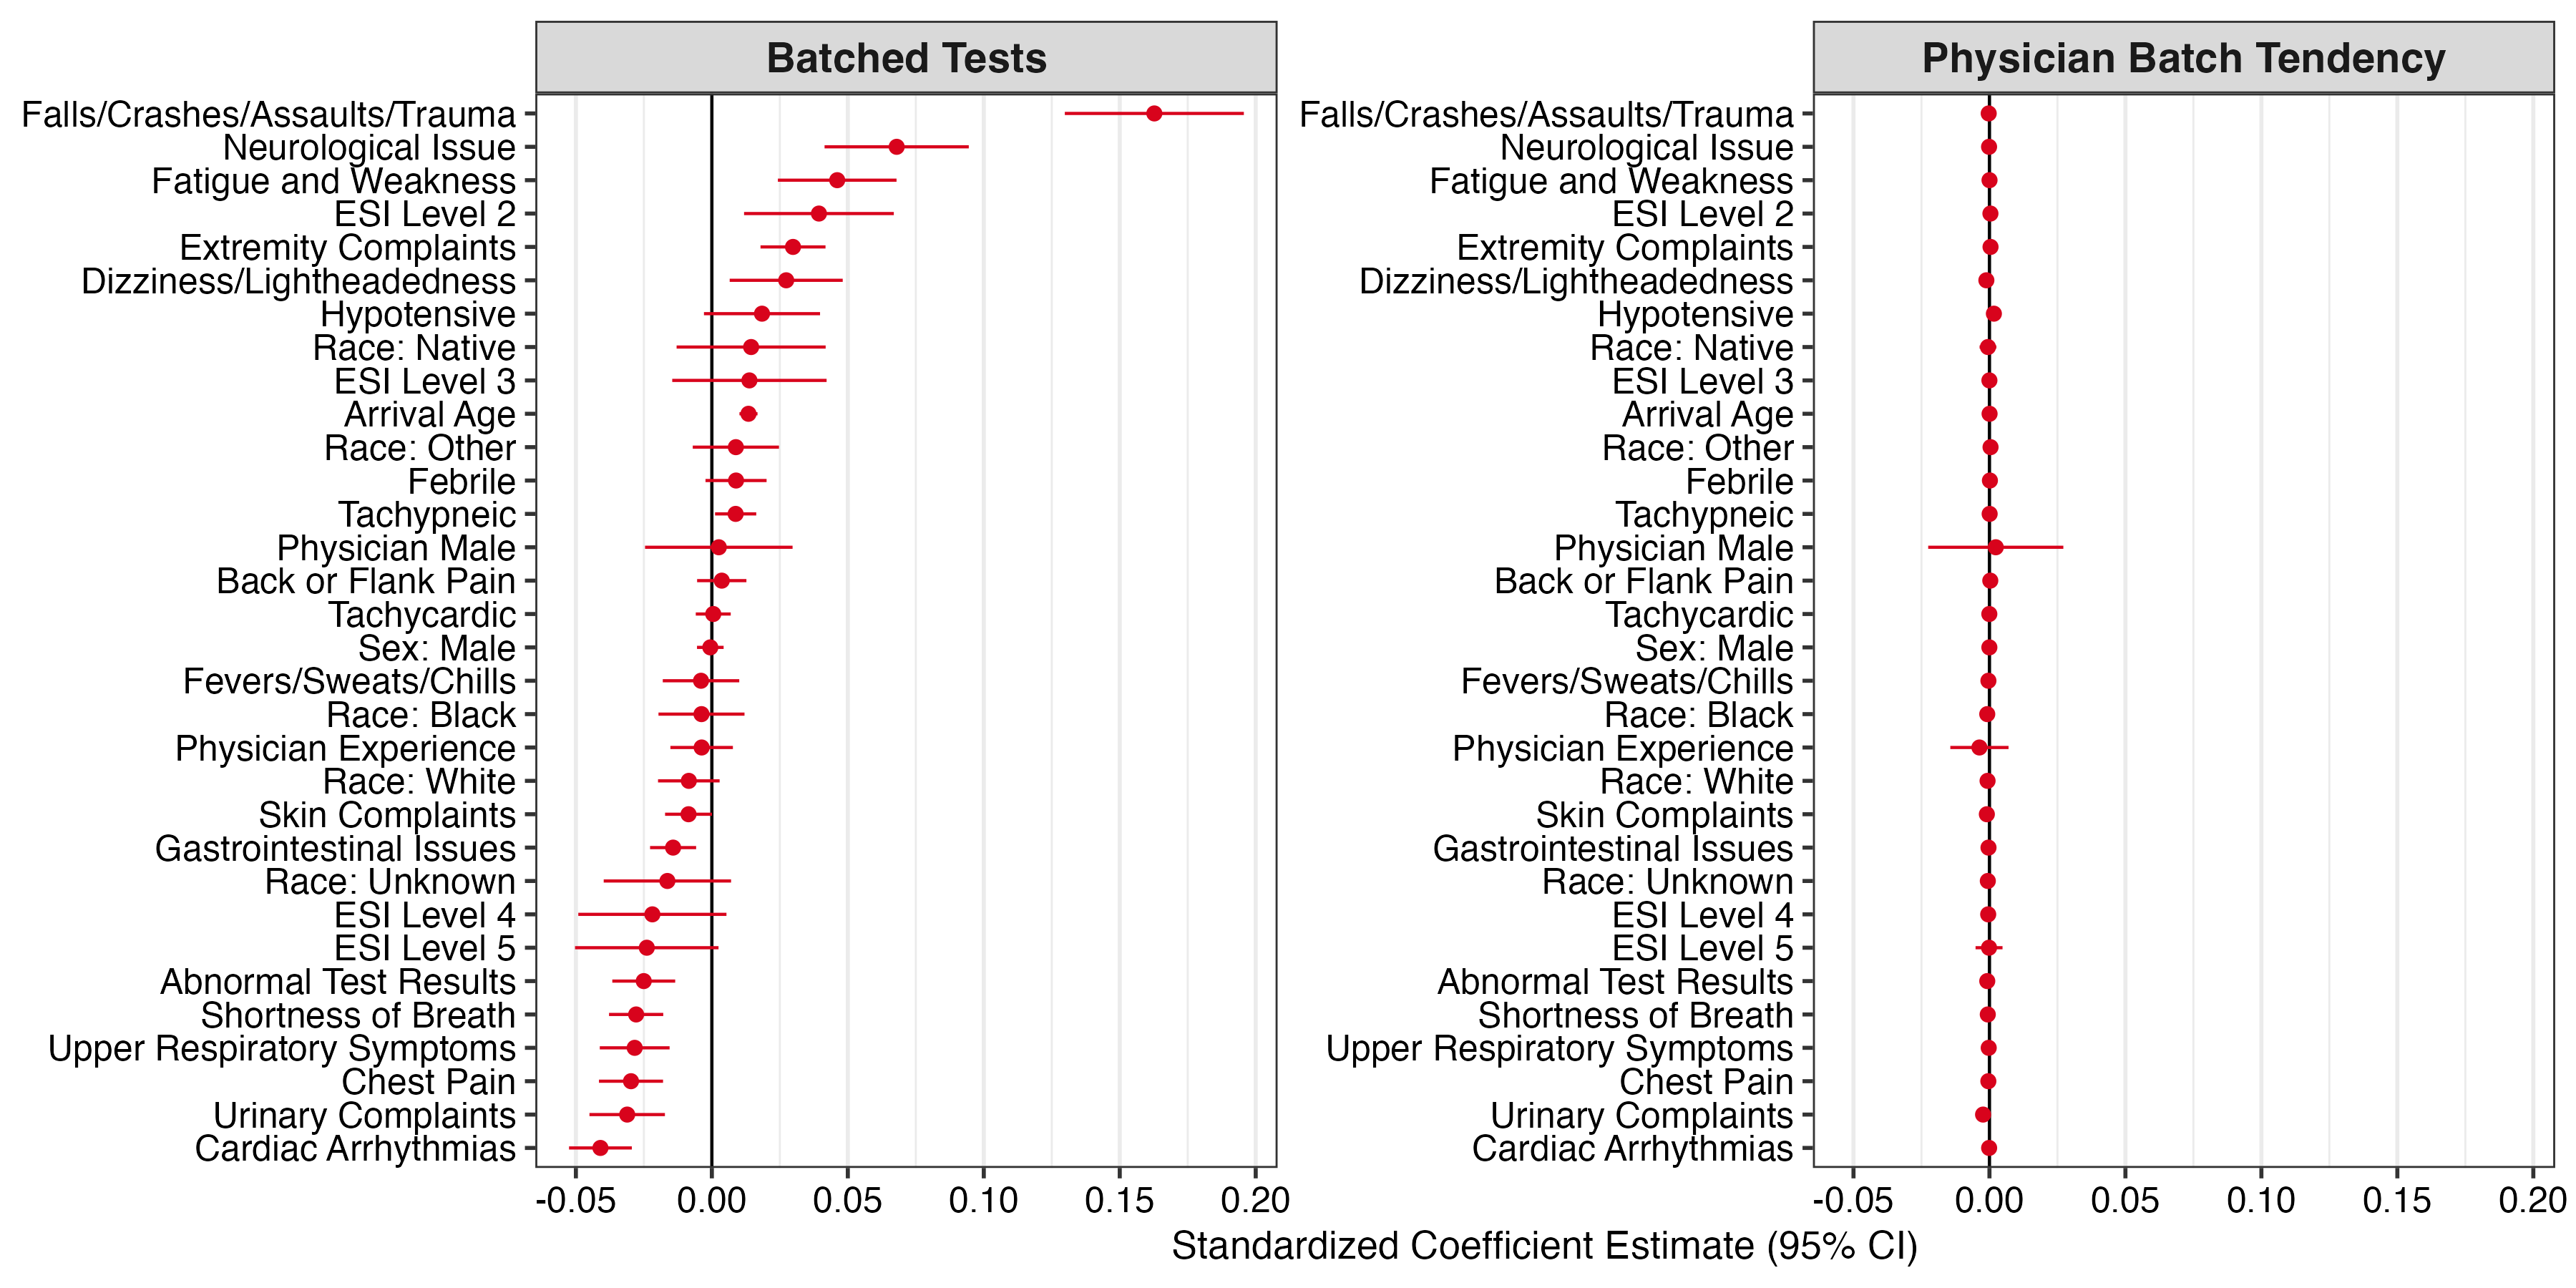
\includegraphics[width=\textwidth]{../outputs/figures/fig2_panel_batched_standardized.png}
    \begin{tablenotes}
        \small
        \item \textit{Notes:} This figure plots a test for quasi-random assignment of patients to physicians in the Mayo Clinic ED. The left panel shows how patient characteristics predict batching decisions. The right panel shows these same characteristics do not predict assignment to physicians with different batch tendencies. Residualization fixed effects include hospital-year-month, hospital-day of week-time of day. Robust standard errors are clustered at the physician level.
    \end{tablenotes}
\end{threeparttable}
\end{figure}

We have added explanatory text in Section 3.3 emphasizing this empirical verification:

\begin{quote}
``Figure 2 provides empirical verification that, while the decision to batch depends on patient characteristics, our measure—batch tendency—is plausibly exogenous. The left panel uses a linear probability model to test whether encounter, patient, ED, and physician characteristics predict the batching decision, controlling for shift-level fixed effects with standard errors clustered at the physician level. As expected, patient characteristics strongly predict batching decisions; for instance, patients with Falls/Assaults/Trauma complaints are 16.2 percentage points more likely to be batched compared to similar patients under similar ED capacity. The right panel assesses whether these same characteristics predict assignment to physicians with different batch tendencies. Importantly, we find that patient characteristics do not significantly predict assignment to high versus low batch-tendency physicians. The coefficients are near zero with confidence intervals crossing zero for all patient characteristics, confirming that, conditional on shift fixed effects (which account for the mechanical rotation), the assignment of patients to physicians with different batching tendencies is effectively random. This validates the rotational assignment mechanism and establishes batch tendency as an exogenous source of variation for identifying causal effects."
\end{quote}


Together, the institutional details and empirical balance tests confirm that Mayo Clinic's rotational assignment mechanism achieves the quasi-randomization necessary for our identification strategy. This distinguishes our study from observational analyses where endogenous patient-physician matching could confound estimates of physician practice effects.

\color{black}



%%%%%%%%%%%%%%%%%%%%%%%%%%%  R1 Comment 5  %%%%%%%%%%%%%%%%%%%%%%%%%%%%%%%%%%
\begin{quote2}
\textbf{R1 Wrote (Potential impact \& writing quality):}

\noindent``The paper is well written, and studies an important question. I hope the authors find this report helpful in moving this work forward.” 
\end{quote2}

\noindent\textbf{***Response:} \textcolor{blue}{We sincerely thank the reviewer for their thorough and constructive feedback. The detailed comments have been invaluable in strengthening our analysis and clarifying our contributions. We believe the extensive revisions addressing the reviewer's concerns about variable definition, empirical strategy, and causal interpretation have substantially improved the manuscript.}


%%%%%%%%%%%%%%%%%%%%%%%%%%%%%%%%%%%%%%%%%%%%%%%%%%%%%%%%%%%%%%%%%%%%%%%%%%%%%%
% End of Reviewer 1 responses
%%%%%%%%%%%%%%%%%%%%%%%%%%%%%%%%%%%%%%%%%%%%%%%%%%%%%%%%%%%%%%%%%%%%%%%%%%%%%%

\clearpage

%%%%%%%%%%%%%%%%%%%%%%%%%%%%%%%%%%%%%%%%%%%%%%%%%%%%%%%%%%%%%%%%%%%%%%%%%%%%%%
%%  SECTION V – RESPONSES TO REVIEWER 2 COMMENTS                           %%
%%%%%%%%%%%%%%%%%%%%%%%%%%%%%%%%%%%%%%%%%%%%%%%%%%%%%%%%%%%%%%%%%%%%%%%%%%%%%%

\pagestyle{fancy}
\fancyhead{}
\fancyhead[RO]{\small{Responses to Referee 2 Comments}}
\renewcommand{\headrulewidth}{0pt}

\noindent\underline{\textbf{IV. Responses to Referee 2 (R2) Comments}}

%%%%%%%%%%%%%%%%%%%%%%%%%%%  R2 Comment 1  %%%%%%%%%%%%%%%%%%%%%%%%%%%%%%%%%%


\begin{quote2}
\textbf{R2 Wrote (Research question \& contribution:):}  

\noindent``The paper’s research question is clear. The main contribution is to provide causal evidence that batch ordering of advanced imaging tests in emergency departments (EDs) — commonly assumed to be efficient — increases patient length of stay (LOS), test volume, and admission rates. EDs are under constant pressure to improve throughput, and advanced imaging is a major driver of delays, costs and overcrowding in the EDs. The paper does have the potential to make a significant and novel contribution by causally examining the impact of diagnostic batch ordering in emergency departments. While prior research has explored physician-driven variation in testing and the operational burden of imaging, this study uniquely isolates the effect of batching behavior using a quasi-randomized design.”
\end{quote2}

\noindent\textbf{Response:} \textcolor{blue}{We appreciate the reviewer's recognition of our contribution to understanding diagnostic test ordering in emergency departments. We agree that challenging conventional assumptions about batch ordering efficiency is important given the operational pressures EDs face. The reviewer's constructive feedback has substantially strengthened our empirical approach and helped us clarify how our quasi-randomized design isolates batching effects from other aspects of physician practice variation.}

\begin{quote2}
\textbf{R2 Wrote (Framing):}  


\noindent``The paper frames the comparison as "batching vs. sequential", but that is not technically correct. In reality, the way the independent variable is defined, the comparison is “early batched imaging” vs. “everything else”, which includes a broad mix of clinical pathways. This muddies the interpretation: are the harms of batching due to: The batching itself? Or just differences between patients who need 2+ early tests vs. those who do not? Moreover, the sequencing is not fully explored: the study favors sequential ordering, but the authors do not actually compare different sequencing strategies or evaluate outcomes where delayed imaging causes diagnostic delays.”
\end{quote2}


\noindent\textbf{Response:} \color{blue}We thank the reviewer for this important clarification about our treatment comparison. The reviewer is absolutely correct that our empirical strategy compares ``early batched imaging" with ``everything else" rather than a pure batching versus sequential comparison. This point was raised by the other reviewers as well. We appreciate this opportunity to clarify our approach and have made substantial revisions to address this concern.

First, an essential clarification: our sample includes only encounters where at least one imaging test was ordered. The "everything else" comparison therefore comprises patients who received either (1) a single imaging test, or (2) multiple tests ordered sequentially—but not patients with zero imaging. This distinction is critical because our comparison is between different imaging strategies for patients requiring diagnostic imaging, not testing versus no testing. That said, the reviewer is correct that our counterfactual remains composite—mixing single-test and sequential multi-test encounters.

The reviewer raises a fundamental question: are the harms from batching itself or from differences between patients needing multiple early tests? This gets to the heart of causal inference in our setting. For decisions at the margin of physciain discretion, such as the one we study, the batching decision is made under uncertainty about whether additional tests will be needed. Conditioning our analysis on eventual test count would introduce post-treatment bias, as the initial ordering strategy causally affects subsequent testing decisions. Our approach preserves causal interpretation by comparing strategies at the moment of decision-making.

We have made the following changes to address your concerns which we believe have made the manuscript stronger:

\begin{enumerate}
    \item \textbf{Reframed our comparison throughout the manuscript}. We now consistently describe our comparison as ``batch ordering versus standard practice" rather than "batching versus sequencing." 
    
    \item \textbf{Clarified what we identify and why it matters}. We added text in Section 3.3 explaining:
    \begin{quote}
    ``Our two-stage least squares estimates represent the LATE of batch ordering for `compliers'---patients whose testing strategy depends on the assigned physician's practice style. This effect compares batch ordering to standard practice, which includes both sequential ordering and single tests. While this involves a composite counterfactual, it provides the policy-relevant parameter: the effect of encouraging comprehensive upfront testing versus allowing diagnostic information to guide testing decisions for patients at the margin of clinical discretion—those whose testing strategy is not dictated by clear clinical necessity but rather depends on physician practice style and judgment."
    \end{quote}
    
    \item \textbf{Added discussion of the information problem}. In Section 3.2.1, we explain why we focus on early batching:
    \begin{quote}
    ``We focus on batches that concern the first imaging tests ordered during the patient encounter because this represents the moment of maximum diagnostic uncertainty, when physicians must decide their testing strategy before clinical information unfolds. Physicians cannot know ex-ante which patients will ultimately require multiple tests, leading to instances of early batching as discretionary choice based on practice style rather than clinical necessity."
    \end{quote}

Regarding potential harms from delayed sequential testing, we find no evidence on 72-hour return, suggesting sequential approaches do not cause harmful diagnostic delays.

\item \textbf{Clarified why ``everything else" is the right comparison}. We added to Section 5.1:
\begin{quote}
    ``This comparison reflects the real choice facing ED managers: should protocols encourage comprehensive upfront testing or preserve diagnostic flexibility? Our estimates show that preserving optionality through standard practice—which allows information from initial tests to guide subsequent decisions—reduces testing intensity."
\end{quote}
\end{enumerate}

The reviewer's observation about mixed clinical pathways in our counterfactual is astute. However, this heterogeneity reflects what makes our estimate policy-relevant. ED managers cannot randomize patients to pure sequential protocols based on eventual diagnostic needs (which are unknown ex-ante). They can only influence whether physicians default to comprehensive early testing or preserve diagnostic optionality when facing uncertainty. Our LATE provides exactly this parameter.

We believe these revisions substantially improve the manuscript's clarity while maintaining scientific rigor. The comparison we identify—batch ordering versus standard practice for marginal patients—is both what we can credibly estimate given the information structure and what policymakers need to know. We are grateful to the reviewer for pushing us to clarify this important distinction, as it has led us to better articulate both the methodological foundations and practical implications of our work.

\color{black}

%%%%%%%%%%%%%%%%%%%%%%%%%%%  R2 Comment 3  %%%%%%%%%%%%%%%%%%%%%%%%%%%%%%%%%%
\begin{quote2}
\textbf{R2 Wrote (Hypotheses):}  

\noindent``As it currently stands, the study lacks a clearly articulated hypotheses section, which would help clarify the underlying mechanisms the authors expect to observe in the results. This section is typically where one would expect the authors to build a narrative around the anticipated behavioral patterns and how those behaviors are theoretically linked to the operational outcomes under study.” 
\end{quote2}

\noindent\textbf{Response:} \color{blue}We thank the reviewer for this valuable suggestion to develop formal hypotheses. The reviewer is absolutely correct that explicitly articulating our theoretical predictions strengthens the paper's contribution and clarifies the mechanisms we expect to observe.

Following this guidance, we have added Section 2.3 ``Hypothesis Development" that builds from our literature review to develop four formal hypotheses about how batch ordering affects ED operations:

\begin{quote}
\subsection*{``Hypothesis Development}

Building on the literature reviewed above, we develop formal hypotheses about how batch ordering affects ED operations. While prior work has identified the mechanisms driving batching behavior and its potential consequences, the net effects remain theoretically ambiguous. Our theoretical framework centers on the fundamental tradeoff between the perceived efficiency of parallel processing and the information value of sequential testing.

\subsubsection*{Information Value and Test Volume}

The decision to batch or sequence tests fundamentally involves whether to preserve the option value of information. Sequential testing allows each test result to inform subsequent decisions, potentially eliminating unnecessary tests. When physicians batch tests upfront, they commit to a diagnostic pathway before information unfolds, forfeiting this option value.

Physicians under high workloads face cognitive strain from task switching and may batch tests to defer complex diagnostic reasoning \cite{kc2013does, skaugset2016can}. However, this cognitive convenience comes at a cost. Without the filtering mechanism of sequential information revelation, physicians must rely solely on their initial assessment. \cite{lam2020why} identify this as a key driver of overtesting---when facing diagnostic uncertainty, physicians order comprehensive test batteries rather than allowing initial results to guide subsequent testing. Given the documented variation in physician testing intensity \cite{hodgson2018are}, with some physicians ordering twice as many tests as their peers, batching likely amplifies these tendencies by removing the natural stopping points that sequential results provide. Therefore:

\begin{quote}
\small
\textit{\textbf{Hypothesis 1.} Batch ordering will increase the total number of imaging tests performed compared to standard practice due to the loss of information value from initial test results.}
\end{quote}

\subsubsection*{Processing Time and Operational Flow}

While batching strategies reduce setup times in manufacturing \cite{Fowler2022}, the ED imaging context presents unique operational constraints as noted in our review. Different imaging modalities require separate equipment and cannot be performed simultaneously \cite{Jessome2020}. This creates a fundamental bottleneck where batched orders must still be executed sequentially, but now with a larger committed workload that cannot be adjusted based on emerging information.

Moreover, the cognitive load literature suggests that processing multiple test results simultaneously increases decision complexity \cite{kc2013does}. When physicians receive multiple results at once rather than sequentially, they must integrate more information simultaneously, potentially lengthening the diagnostic reasoning process. This "information overload" effect, combined with the additional tests ordered as predicted in H1, suggests that batching may paradoxically increase rather than decrease processing times:

\begin{quote}
\small
\textit{\textbf{Hypothesis 2.} Batch ordering will increase patient length of stay and time to disposition compared to standard practice, as the operational constraints of imaging and increased test volume outweigh any potential benefits of parallel processing.}
\end{quote}

\subsubsection*{Clinical Decision-Making and Disposition}

The medical literature recognizes ``diagnostic momentum"---where abnormal findings, even if clinically insignificant, drive further workup and more conservative clinical decisions \cite{coen2022clinical, featherston2020decision}. When physicians batch order and receive multiple results simultaneously, they encounter more opportunities for incidental findings that may influence disposition decisions \cite{lumbreras2010incidental, berlin2011incidentaloma}. As our review noted, physicians facing uncertainty and potential legal consequences may opt for more conservative disposition decisions \cite{rao2012overuse, lam2020why}. The simultaneous arrival of multiple test results, particularly with incidental findings, may trigger defensive medicine behaviors:

\begin{quote}
\small
\textit{\textbf{Hypothesis 3.} Batch ordering will increase hospital admission rates through increased diagnostic intensity and the influence of incidental findings on clinical decision-making.}
\end{quote}

\subsubsection*{Contextual Moderators}

The literature on physician behavior under capacity constraints consistently shows that resource scarcity forces more selective decision-making \citep{kuntz2014stress, kc2009impact}. When EDs face severe overcrowding, the operational pressures documented in our review intensify. Under these conditions, physicians may reserve batching for cases where it is clinically essential rather than convenient:

\begin{quote}
\small
\textit{\textbf{Hypothesis 4.} The effects of batch ordering on LOS and test volume will be attenuated under conditions of major ED overcapacity, as physicians become more selective in their batching decisions.}
\end{quote}

These hypotheses provide testable predictions that we examine using our quasi-experimental design. By leveraging variation in physician batching tendency under random patient assignment, we can identify whether these theoretical mechanisms manifest in actual ED operations."
\end{quote}

This new section provides the theoretical foundation that motivates our empirical specifications and helps readers understand which mechanisms we test. We are grateful to the reviewer for this suggestion, which has substantially strengthened the manuscript's theoretical contribution.

\color{black}


%%%%%%%%%%%%%%%%%%%%%%%%%%%  R2 Comment 4  %%%%%%%%%%%%%%%%%%%%%%%%%%%%%%%%%%
\begin{quote2}
\textbf{R2 Wrote (Shift‑of‑testing to other settings):}  
``While the study finds that batch ordering increases imaging in the ED as well as inpatient admissions, it does not evaluate whether this reflects actual overuse or a shift in imaging from the inpatient setting to the ED. In other words, it is unclear whether batching increases unnecessary testing or simply frontloads diagnostics."

\end{quote2}

\noindent\textbf{Response:} \color{blue}We thank the reviewer for this important distinction between overuse and frontloading of diagnostics. The reviewer is correct that we cannot definitively determine whether the additional imaging represents unnecessary testing or simply shifts testing from inpatient to ED settings. This is an important limitation of our study.

However, interpreting our findings purely as frontloading faces a conceptual challenge. Frontloading would imply batched patients receive ED tests that would have been ordered during a predetermined hospitalization. Yet admission itself is a downstream consequence of the testing strategy in our data—we find that batching increases admission probability through increases in imaging tests performed. This suggests at least some proportion of the additional tests are driving new admission decisions rather than frontloading diagnostics for patients who would have been admitted regardless of their ED imaging results. That is, the tests themselves are creating admissions, not being ordered because admission was already determined.

That said, we acknowledge multiple causal pathways may operate simultaneously. Some batched patients may receive tests that genuinely reveal admission-worthy conditions that would have been discovered later. Others may be admitted defensively due to incidental findings from comprehensive imaging that would not have been pursued under sequential testing. Without linked inpatient imaging records, we cannot empirically separate these mechanisms.

We have been careful throughout the manuscript to avoid characterizing the additional tests as "waste" or "overuse," as our LATE identifies effects for marginal patients whose testing decisions vary by physician preference—these tests may have clinical value regardless of timing. However, even if batching represents frontloading rather than overuse, it has operational consequences worth noting. Based on discussions with our physician coauthors at both study sites: ED imaging resources are typically more constrained than inpatient resources, frontloading increases ED congestion and delays care for other ED patients, and inpatient teams often prefer directing their own diagnostic approach based on evolving clinical information.

We have added discussion of this limitation in Section 5.3:

\begin{quote}
"We cannot determine the extent to which the additional imaging from batching represents unnecessary testing or frontloading of diagnostics that would eventually occur in the inpatient setting. However, interpreting our findings purely as frontloading is complicated by the fact that admission itself is affected by batching—we observe a 39 percentage point increase in admission probability, suggesting the tests themselves influence disposition decisions. Multiple mechanisms may operate: some additional tests may reveal genuine admission-worthy conditions, while others may trigger defensive admissions through incidental findings. Distinguishing between these pathways would require linked ED-inpatient imaging data to examine whether batched patients receive correspondingly fewer tests after admission. This remains an important direction for future research."
\end{quote}

We appreciate the reviewer highlighting this distinction, as it has led us to be more precise about the causal pathways our estimates capture and the important questions that remain for future research.

\color{black}

%%%%%%%%%%%%%%%%%%%%%%%%%%%  R2 Comment 5  %%%%%%%%%%%%%%%%%%%%%%%%%%%%%%%%%%
\begin{quote2}
\textbf{R2 Wrote (Request for cost‑benefit analysis):} 

\noindent``Relatedly, what would help is a cost-benefit analysis -- given the
findings about overuse, it is surprising the paper does not estimate financial impact or
imaging cost burdens. Do the authors have any data they could use to conduct such an
analysis?” 
\end{quote2}

[PLACEHOLDER I WANT TO CHECK WITH SOROUSH FIRST]

%%%%%%%%%%%%%%%%%%%%%%%%%%%  R2 Comment 6  %%%%%%%%%%%%%%%%%%%%%%%%%%%%%%%%%%
\begin{quote2}
\textbf{R2 Wrote (Batch timing and its relation to LOS):}

\noindent``Batch timing is unclear to me. Specifically, Length of Stay (LOS) is used as a primary outcome. Batching, defined as imaging orders within the first 5 minutes of encounter, is treated as a treatment applied at the beginning of the visit. But in real ED workflows, the decision to batch may itself be a function of how the patient’s case has unfolded up to that point. For example, if the diagnosis is taking longer, or prior tests have not resolved the issue, or if the physician senses the patient may be admitted soon, then the physician might batch several tests later in the encounter in order to “wrap things up” and avoid delays — i.e., batching becomes a consequence of extended LOS, not just a cause. The 5-minute window may not capture the delayed batching; e.g., if initial results come back inconclusive or the patient’s condition worsens. Thus, the batching variable may be misclassified, and later batches that react to prolonged stays are excluded from the analysis. Even when orders are placed early, test results often take time to return. That delay — especially from CTs or MRIs — inflates LOS. Therefore, the measured LOS may not be a clean posttreatment outcome, but instead partially determined by the batching process itself. This risks simultaneity bias, where cause and effect are entangled in time. The issue is less severe if the paper really only claims to understand something about initial batching decisions, but I am not sure the authors have made those distinctions clear enough.” 
\end{quote2}

\noindent\textbf{Response:} \color{blue}We thank the reviewer for this insightful observation about the temporal relationship between batching and LOS. Before addressing the specific timing concerns, we note that in response to feedback from all three reviewers about our original specification, we have substantially expanded our control set to better isolate imaging-specific effects. Our revised primary specification now includes physician characteristics (experience, gender, hours into shift) and laboratory test ordering to address concerns that our instrument might capture general diagnostic intensity rather than batching-specific behavior. 

This more conservative specification attenuates our time-based estimates while the mechanism (imaging volume) remains highly significant. Our revised estimates show batching increases imaging tests by 91\% (1.214 additional tests, p<0.001), with point estimates suggesting 79\% longer LOS (p=0.089) and 88\% longer time to disposition (p=0.172). However, these time effects are no longer statistically significant at conventional levels. We emphasize these revised estimates throughout our responses. Despite this attenuation, the temporal relationship concerns that the reviewer raises remain important to address, as they relate to our research design, regardless of effect magnitude.

\textbf{Why early batching is the relevant parameter:} The reviewer correctly notes that physicians might batch tests later to ``wrap things up." This adaptive behavior is fundamentally different from the discretionary decision to order comprehensive imaging upfront. Our instrumental variable (physician batch tendency) specifically captures variation in early ordering propensity—identifying physicians who habitually commit to comprehensive imaging before information unfolds versus those who preserve diagnostic flexibility.

Empirically, we verify that ``late batching"—cases where a batch follows a single test—is rare, occurring in only 189 encounters (1.91\% of multi-test encounters). To verify this classification does not impact our results, we re-estimated all models treating such cases as batched (Appendix D). The results are virtually identical.

\textbf{Clarifications made throughout the manuscript:} Following the reviewer's observation, we have revised our framing to emphasize that our parameter of interest is the effect of discretionary batching versus standard practice:

\begin{enumerate}
\item \textbf{Abstract:} Now specifies "discretionary batching decisions made at encounter initiation"

\item \textbf{Section 1.2:} Clarifies that our LATE identifies "the effect of discretionary batching for patients whose testing strategy depends on physician practice style rather than clinical necessity"

\item \textbf{Section 3.2.1:} Extensively revised to clarify our focus:
\begin{quote}
"We focus on batches that concern the first imaging tests ordered during the patient encounter because this represents the moment of maximum diagnostic uncertainty when physicians must decide their testing strategy before clinical information unfolds. Physicians cannot know ex-ante which patients will ultimately require multiple tests, making early batching a discretionary choice based on practice style rather than clinical necessity."
\end{quote}
\end{enumerate}

\textbf{LOS as outcome and simultaneity bias:} The reviewer raises an important concern about whether LOS can serve as a clean post-treatment outcome given that test completion times mechanically contribute to its measurement. We acknowledge this concern but emphasize that this relationship is not a confounder—it is precisely the causal pathway our study seeks to identify.

The reviewer asks whether this creates ``simultaneity bias, where cause and effect are entangled in time." This would be a concern if some third factor simultaneously determined batching and LOS, or if LOS caused batching. However, our design addresses this: we focus on early discretionary batching decisions (the first tests ordered during the encounter), and our instrument (physician batch tendency) is predetermined before the patient encounter begins. The temporal ordering is clear: physician tendency $\rightarrow$ batching decision $\rightarrow$ test ordering $\rightarrow$ test completion $\rightarrow$ LOS. The mechanical relationship between test completion and LOS represents the causal pathway through which early batching operates, not simultaneity bias.

Our treatment is the decision to batch, and LOS captures the total consequences of that decision. When physicians choose to batch tests upfront, they set in motion a cascade of operational consequences: patients wait for multiple tests to complete, radiologists must interpret multiple images, physicians must cognitively process all results simultaneously, and clinical decisions must integrate potentially conflicting or incidental findings. These are the mediating mechanisms through which early batching decisions affect patient flow.

To further separate clinical decision-making time from test completion time, we examine "time to disposition"—the duration until physicians make admission/discharge decisions, excluding post-decision boarding. While our revised estimates show economically large but imprecisely estimated effects (88\% increase, p = 0.172), the fact that time to disposition—which excludes post-decision boarding—shows similar point estimates to total LOS, demonstrates that early batching affects not only mechanical test completion waiting but also clinical processing efficiency. Even when excluding post-disposition time (during which no testing occurs), the early discretionary batching decision yields substantial point estimates for delays in clinical decision-making, although we acknowledge that these effects are measured with uncertainty in our more conservative specification.

We appreciate the reviewer's careful attention to these temporal dynamics, which has prompted us to more clearly articulate that our study evaluates the full operational consequences of discretionary early batching decisions—precisely the parameter ED managers need to understand when considering protocols to influence physician ordering behavior.

\color{black}


%%%%%%%%%%%%%%%%%%%%%%%%%%%  R2 Comment 7  %%%%%%%%%%%%%%%%%%%%%%%%%%%%%%%%%%
\begin{quote2}
\textbf{R2 Wrote (Definition of batching):}  
``The definition of batching is also narrowly defined to be 2+ tests ordered within the 5 first minutes. The study equates batch ordering with guaranteed test completion and additive imaging volume. However, in practice, test results may return asynchronously, and physicians may update their diagnostic plans based on early results—even for batched orders. For example, even if the physicians initially batch ordered the tests, they could cancel some of these as they review the results. The paper would benefit from clarifying how often batched tests were actually completed and whether sequential result review modified downstream test execution. Without this, the causal link between batch ordering and increased imaging intensity may be overstated.” 
\end{quote2}

\noindent\textbf{Response:} \color{blue}
We thank the reviewer for this important clarification question. Our outcome measures count imaging tests actually performed, not merely ordered. This critical distinction strengthens our causal interpretation: the 1.2 additional tests per marginally batched patient represent completed imaging studies that consumed resources and time, not provisional orders subsequently cancelled.

Based on consultation with our physician coauthor at Mayo Clinic, test cancellations after batch ordering face substantial operational barriers. Once the radiology department acknowledges an order, cancellation requires physicians to physically call and request the department to "push back" the imaging order. Furthermore, radiology departments often coordinate between modalities (e.g., CT and ultrasound) so patients move directly from one scanner to another. With radiologist read times averaging 60 minutes, patients typically complete all batched imaging before initial results become available for physician review. While cancellations occasionally occur (e.g., a CT scan revealing appendicitis leading to a cancelled pelvic ultrasound), the operational friction makes these exceptions rather than the standard practice.

Importantly, even if some batched orders were cancelled, this would render our estimates conservative. Cancelled tests still consume operational resources—patients are queued, transported, and prepared for imaging that ultimately does not occur. These inefficiencies from cancelled tests would represent an additional operational burden beyond what our completed test counts capture. Thus, our measure of performed tests likely represents a lower bound on the actual operational impact of batching behavior.

\textbf{Manuscript changes made throughout:}

We have clarified the distinction between ordered and performed tests in multiple sections:

Section 3.2.2 (Dependent Variables): 
\begin{quote}
``Beyond time-based metrics, we examine resource utilization through the number of distinct imaging tests performed during each ED encounter. This count variable helps us understand how batch ordering practices influence the diagnostic workload."
\end{quote}

Section 4.2 (Results): Added clarification: 
\begin{quote}
``Discretionary batching also leads to more intensive diagnostic testing. Specifically, the marginal batched patient receives 1.2 more distinct imaging tests (completed studies with documented results), representing a 91\% increase from the mean for standard care patients."
\end{quote}

Table 4: Added footnote: 
\begin{quote}
``Test counts represent performed imaging studies with documented results, not ordered tests. The persistence of increased test volume under batching suggests cancellations do not substantially offset the effect."
\end{quote}

Section 5.3 (Limitations): Added: 
\begin{quote}
``Our data contains imaging tests that were both ordered and performed. We cannot observe tests that were ordered but subsequently cancelled before completion. However, test cancellation after ordering requires substantial coordination—physicians must call the radiology department to remove patients from imaging queues. This operational friction makes cancellations rare. Moreover, cancelled tests introduce their own inefficiencies: patients experience delays from queuing and preparation, while ED resources are allocated to coordinate cancellations. To the extent that batched orders are more likely to include tests that are ultimately cancelled, our estimates of performed tests would understate the true operational burden of batching behavior."
\end{quote}

These clarifications ensure that readers understand our analysis captures actual resource utilization and that potential cancellations would, if anything, strengthen rather than weaken our conclusions about the operational burden of batching.

\color{black}

%%%%%%%%%%%%%%%%%%%%%%%%%%%  R2 Comment 8  %%%%%%%%%%%%%%%%%%%%%%%%%%%%%%%%%%
\begin{quote2}
\textbf{R2 Wrote (Role of laboratory results):}  

\noindent``While the study restricts its scope to imaging due to its operational constraints, it does not address the interplay and potential dependencies between imaging and other diagnostic inputs—particularly lab results. One can imagine that in practice, lab results often arrive earlier and may prompt physicians to reassess imaging decisions, even when tests are initially batched. Could this potentially overstate the causal impact of batching on downstream outcomes?” 
\end{quote2}

\noindent\textbf{Response:} \color{blue}
We thank the reviewer for raising this important concern about whether earlier-arriving lab results might affect our estimates of batching's causal impact. This insightful observation prompted us to empirically examine the potential interplay between laboratory and imaging pathways, which has strengthened our analysis.

\textbf{Empirical test of lab-imaging interplay:} In response to similar concerns from Reviewer 1 about whether our instrument captures general diagnostic intensity rather than imaging-specific behavior, we substantially expanded our specification to include laboratory test ordering as a control variable. This directly tests the mechanism the reviewer describes.

If batch tendency simply reflected physicians who order comprehensive diagnostics across all modalities—with labs potentially modifying imaging pathways—then controlling for whether labs were ordered should substantially attenuate our imaging effects. However, our results show imaging volume effects remain large and highly significant (1.214 additional tests, p<0.001) even after controlling for laboratory utilization.

This pattern demonstrates that while batch tendency does correlate with some general diagnostic intensity (as evidenced by the first-stage attenuation), substantial imaging-specific variation persists after accounting for laboratory pathways. In other words, physicians with high batch tendencies order more imaging even when we compare patients who received identical laboratory workups. This directly addresses the reviewer's concern: the lab-imaging interplay does not substantially confound our estimates because we explicitly control for it.

The reviewer correctly notes that lab results often arrive before imaging results (typically 30-60 minutes for basic labs versus 90-165 minutes for imaging). Based on consultation with our physician co-author at the Mayo Clinic, normal lab results typically do not lead to imaging cancellation. Cancellation occurs only in rare, extreme cases: when labs provide a definitive diagnosis (e.g., severe anemia fully explaining dyspnea, thereby eliminating the need for a chest CT) or when results indicate instability precluding imaging (e.g., severe hyperkalemia requiring immediate dialysis). More commonly, abnormal lab results might modify the imaging type—for instance, switching from contrast to non-contrast CT for acute kidney injury—but do not eliminate the need for imaging. Importantly, even these modifications require physicians to call the radiology department, creating a significant workflow barrier that discourages treating batch orders as provisional.

Given these operational realities, imaging cancellations based on lab results are rare. Our outcome measures count performed tests, not ordered tests, so any cancellations that do occur would make our estimates conservative—we would be understating the initial commitment to imaging that batching represents. The fact that we observe 1.2 additional performed imaging tests per marginally batched patient demonstrates that  batched imaging pathways, once initiated, proceed to completion despite the theoretical possibility of modification based on lab results.

\textbf{Manuscript changes made:}

To reflect this enhanced specification and address concerns about lab-imaging interplay, we have made the following revisions:

\begin{enumerate}
\item \textbf{Enhanced primary specification (Table 4):} Our revised main results now include laboratory test ordering as a control variable. Column 5 shows our primary 2SLS specification controlling for patient characteristics, physician characteristics, hours into shift, and laboratory tests performed. The persistence of large, significant imaging effects (1.214 tests, p<0.001) demonstrates imaging-specific variation.

\item \textbf{Expanded methods discussion (Section 3.3):} We added detailed explanation of our control strategy:
\begin{quote}
"Our revised primary specification includes realized diagnostic intensity measured by whether laboratory tests were performed during the encounter. This control directly addresses concerns that batch tendency might reflect general diagnostic aggressiveness rather than imaging-specific timing decisions. The persistence of imaging effects after controlling for laboratory utilization demonstrates that our instrument captures variation specific to imaging workflows."
\end{quote}
\end{enumerate}

These revisions demonstrate that the lab-imaging interplay the reviewer describes does not confound our estimates, as we explicitly control for laboratory pathways in our primary specification.
\color{black}



%%%%%%%%%%%%%%%%%%%%%%%%%%%  R2 Comment 9  %%%%%%%%%%%%%%%%%%%%%%%%%%%%%%%%%%
\begin{quote2}
\textbf{R2 Wrote (Limited scope of patient conditions):}  
 
\noindent``The study excludes many complaints where imaging is rarely ordered or batching is infeasible (e.g., dermatologic issues, urinary complaints). The results may not apply to low-acuity patient populations or fast-track EDs. Therefore, the study is more narrowly defined.” 
\end{quote2}

\noindent\textbf{Response:} \color{blue}We thank the reviewer for highlighting the focused nature of our sample. The reviewer is correct that we exclude complaints where imaging is rarely ordered or batching is uncommon (occurring less than 5\% of the time). This exclusion was necessary for both statistical and substantive reasons.

Statistically, our instrumental variables approach requires sufficient variation in batching behavior to identify effects. Including complaints where batching rarely occurs time would create weak instrument problems and yield unreliable estimates. For these rarely batched complaints, physicians have effectively determined that batching is clinically inappropriate—there is no discretionary decision to be made.

Substantively, the random assignment of patients to physicians at Mayo Clinic allows us to restrict our sample to complaints where batching is a relevant operational decision without introducing selection bias. This focused approach provides clear, actionable insights for specific clinical scenarios—trauma, neurological complaints, abdominal pain—where batching decisions are actively debated among emergency physicians and meaningfully impact ED operations. These complaints represent approximately 25\% of the ED volume but account for 41\% of imaging resource utilization in our data, underscoring their operational significance.

We agree that this narrows the scope of our study. However, this focus ensures our estimates are both statistically identified and operationally relevant for the clinical contexts where batching represents a genuine debated practice choice. We have added text to the limitations section explicitly acknowledging this scope:

\begin{quote}
``Our findings apply to moderate-to-high acuity patients with complaints commonly requiring multiple imaging studies. The effects of batching in low-acuity or fast-track settings, where imaging is less common, remain unexplored."
\end{quote}


\color{black}

%%%%%%%%%%%%%%%%%%%%%%%%%%%  R2 Comment 10  %%%%%%%%%%%%%%%%%%%%%%%%%%%%%%%%%
\begin{quote2}
\textbf{R2 Wrote (Physician‑only ordering \& staffing mix):}  

\noindent``At Mayo, only emergency physicians (EPs) order imaging, which is not standard in many EDs (where nurse practitioners, physician assistants, or residents contribute). Does this limit the generalizability to other care settings? How does this difference manifest itself particularly in EDs with significant staffing by parttime or mid-level providers?” 
\end{quote2}

\noindent\textbf{Response:} \color{blue}We appreciate the reviewer raising this important point about staffing differences across EDs. The reviewer is correct that Mayo Clinic's physician-only ordering policy differs from many EDs, where nurse practitioners, physician assistants, and residents participate in ordering decisions.

However, our replication at MGH addresses this concern of generalizability directly. MGH employs a mixed staffing model where mid-level providers participate under attending supervision—more representative of typical US emergency departments. As shown in Table 7, the effects at MGH (a 44.3\% increase in LOS and 1.8 additional tests) are directionally similar and statistically indistinguishable from those at Mayo, demonstrating that the batching phenomenon persists across different staffing configurations.

Mayo's physician-only setting provides methodological advantages for causal identification by eliminating potential confounding from provider-type variation (e.g., systematic differences in ordering patterns between nurse practitioners and attending physicians) and ensuring all decisions reflect experienced clinical judgment. The random assignment mechanism is also simpler because patients cannot be triaged to different provider types based on acuity or complaint. The consistency of results at MGH—despite its more complex staffing environment—validates that batching effects persist when mid-level providers participate in care delivery.

Our physician co-authors at both sites confirm that, while ordering processes differ, the fundamental trade-offs of batching versus sequential testing remain similar across settings. That said, we acknowledge that EDs with predominantly mid-level staffing may face additional dynamics not fully captured in our analysis, such as supervision requirements or handoff patterns that could interact with batching decisions. We have added text to Section 4.6:

\begin{quote}
``While Mayo Clinic's physician-only ordering differs from many EDs, this provides cleaner identification of batching effects. Our replication at MGH—with its mixed staffing model including mid-level providers—demonstrates that these effects persist across different provider configurations, though the specific dynamics in EDs with predominantly mid-level staffing warrant future research."
\end{quote}
\color{black}


%%%%%%%%%%%%%%%%%%%%%%%%%%%  R2 Comment 11  %%%%%%%%%%%%%%%%%%%%%%%%%%%%%%%%%
\begin{quote2}
\textbf{R2 Wrote (Sensitivity of results – Table 4):}  

\noindent``I would urge the authors to discuss the difference in results between column 4 and 5 of Table 4, specifically with regards to sensitivity to influential controls, since the results before and after adding controls differ significantly."
\end{quote2}

\noindent\textbf{Response:}\color{blue}
We thank the reviewer for this important observation. In response to concerns from all three reviewers about our original specification, we substantially expanded the control set in our primary specification (Table 4, Column 5). The differences between columns 4 and 5 reflect this enhancement.

\textbf{What changed in Column 5:}Our revised baseline controls now include:
\begin{itemize}
\item Patient characteristics: vital signs, age, demographics, chief complaint severity
\item Physician characteristics: experience, gender, hours into shift
\item Realized diagnostic intensity: laboratory tests performed
\item Contextual factors: ED capacity level, temporal fixed effects
\end{itemize}

\textbf{Comparing columns 4 and 5:}

\begin{itemize}
\item \textbf{Imaging volume effects persist:} 1.360*** → 1.214*** (both p<0.001). The mechanism remains highly significant and economically large despite comprehensive controls.
\item \textbf{Time effects attenuate:} Log LOS changes from 0.679** (p<0.05) to 0.580 (p=0.089).
\item \textbf{Admission effects stable:} 0.397*** → 0.392*** (both p<0.001). The disposition effects remain highly significant and virtually unchanged in magnitude.
\item \textbf{Quality metrics unchanged:} 72-hour returns show identical null effects across specifications.
\end{itemize}
We have added a discussion of this specification sensitivity in Section 4.1 (Results), and our response to Reviewer 1 provides detailed progressive control tables showing how estimates change as each control set is added (Appendix D).
\color{black}

%%%%%%%%%%%%%%%%%%%%%%%%%%%  R2 Comment 12  %%%%%%%%%%%%%%%%%%%%%%%%%%%%%%%%%
\begin{quote2}
\textbf{R2 Wrote (Table 1 labeling issue):}  

\noindent``In Table 1, the independent variable and dependent variable seem reversed.” 
\end{quote2}

\noindent\textbf{Response:} \color{blue}
We thank the reviewer for catching this labeling error. We have corrected the table to properly display ``Batched" as the dependent variable and ``Batch Tendency" as the independent variable. The table now clearly shows the first-stage relationship where physician batch tendency predicts the probability of batching for a given patient encounter. We apologize for any confusion this may have caused.
\color{black}

%%%%%%%%%%%%%%%%%%%%%%%%%%%  R2 Comment 13  %%%%%%%%%%%%%%%%%%%%%%%%%%%%%%%%%
\begin{quote2}
\textbf{R2 Wrote (Potential impact \& writing):}  

\noindent``The insights are policy-relevant, as they directly inform how EDs might design decision support tools, diagnostic protocols, or physician feedback systems to reduce overuse and streamline care. While the methodological innovation (a quasi-experimental IV strategy using random physician assignment) may not be groundbreaking in design, its application to clinical operations and diagnostic behavior is well-executed, adding credibility and potential for translation.” 
\end{quote2}

\noindent\textbf{Response:} \color{blue}
We thank the reviewer for this encouraging assessment of our work's policy relevance and execution. We agree that the key contribution lies not in methodological innovation per se, but in applying rigorous causal inference methods to an important operational decision in emergency medicine that has long been debated. We are grateful that the reviewer sees the potential for our findings to inform practical interventions such as decision support tools and physician feedback systems. In response to this and other reviewers' suggestions, we have strengthened the policy implications section to provide more concrete guidance for ED managers considering interventions to optimize diagnostic test ordering practices.
\color{black}


%%%%%%%%%%%%%%%%%%%%%%%%%%%%%%%%%%%%%%%%%%%%%%%%%%%%%%%%%%%%%%%%%%%%%%%%%%%%%%
% End of Reviewer 2 responses
%%%%%%%%%%%%%%%%%%%%%%%%%%%%%%%%%%%%%%%%%%%%%%%%%%%%%%%%%%%%%%%%%%%%%%%%%%%%%%
\clearpage




\pagestyle{fancy}
\fancyhead{}
\fancyhead[RO]{\small{Responses to Referee 3 Comments}}
\renewcommand{\headrulewidth}{0pt}

\noindent\underline{\textbf{V. Responses to Referee 3 (R3) Comments}}

%%%%%%%%%%%%%%%%%%%%%%%%%%%  R3 Comment 1  %%%%%%%%%%%%%%%%%%%%%%%%%%%%%%%%%%


\begin{quote2}
\textbf{R3 Wrote (Research question \& contribution:):}  

\noindent``Given the growing concern about overdiagnosis in general and its potential role in exacerbating ED overcrowding, I find the research question of this paper highly relevant to emergency medicine management. Due to the individualistic nature of decision-making in EDs, emergency physicians are often perceived as “cowboy doctors.” While it may be challenging to implement strict guidelines for test-ordering behaviors in such a dynamic setting, I believe that providing empirical evidence on how ED physicians’ decision-making affects system performance can be eye-opening and may encourage more informed behavior where feasible. Thus, this paper has the potential to make a meaningful contribution to the practice and management of emergency medicine. However, I have serious concerns about the empirical strategy employed in this paper, which raise questions about the validity of the findings. I outline my comments in detail below, with the hope that they will help the authors strengthen their work.”
\end{quote2}

\noindent\textbf{Response:} \color{blue}
We sincerely appreciate the reviewer's recognition of our paper's relevance to emergency medicine management and the important problem of overdiagnosis in contributing to ED overcrowding. We are grateful for your detailed methodological comments, which have substantially strengthened our work. In response to your concerns about the empirical strategy, we have: (1) implemented physician fixed effects as an alternative instrument construction as you suggested, (2) added additional physician level controls to our main specification, (3) added robustness checks using alternative model specifications, (4) provided detailed sample selection documentation, and (5) included heterogeneity analyses by complaint. We believe these revisions, detailed in our responses below, now provide the robust empirical foundation necessary to support our findings. We hope you find the strengthened methodology addresses your concerns.
\color{black}

\color{black}

\begin{quote2}
\textbf{R3 Wrote (Major concern - Instrumental variable):}  

\noindent``While the authors show that the proposed IV satisfies the relevance condition, I am not convinced that it satisfies the exclusion restriction. Specifically, “batchers” and “sequencers” may differ in their performance in ways that influence the outcome measures—not solely through the batching decision for the focal patient. This means that the IV might be capturing other aspects of physician behavior, which could bias the results.

Although the authors attempt to address this concern through a placebo test in the Appendix, the subsample used for this test appears to differ substantially from the main sample in terms of clinical conditions and outcome measures (comparing Tables 3 and D1). I encourage the authors to explore alternative IVs that better satisfy both the relevance condition and exclusion restriction.

On another point related to the proposed IV, the authors construct the IV using the residual from Equation (1). Although this model accounts for time fixed effects (FE) and observable patient and clinical characteristics, it does not account for unobserved non-physician-specific factors that may also be captured by the residuals. To more accurately estimate the physician-specific effect on batching decisions, I recommend that the authors include physician fixed effects in this model.

Similarly, to control for physician-specific characteristics where possible, I recommend including physician fixed effects in all models throughout the paper."
\end{quote2}

\noindent\textbf{Response:} \color{blue}We appreciate the reviewer's careful attention to whether our instrument satisfies the exclusion restriction. The reviewer's concern—that batchers and sequencers may differ in performance in ways beyond batching decisions—is exactly right to scrutinize. All three reviewers raised this same concern, and in response, we have substantially strengthened our identification strategy. We address the exclusion restriction concern first, then discuss the alternative instrument construction using physician fixed effects.

The reviewer is correct that if batch tendency captures other aspects of physician behavior (general diagnostic aggressiveness, thoroughness, experience-based practice patterns), this would bias our results. In our original specification, we controlled only for patient characteristics (vital signs, age, demographics, chief complaint severity) and temporal factors (shift-level effects). In response to concerns from all three reviewers, we have substantially expanded our control set to test whether batch tendency reflects general diagnostic intensity versus imaging-specific timing decisions.

Our revised primary specification now includes:

\begin{itemize}
\item \textbf{Patient characteristics:} Vital signs (tachycardic, tachypneic, febrile, hypotensive), age, demographics, chief complaint severity
\item \textbf{Physician characteristics:} Years of experience, gender, hours into shift (capturing potential fatigue effects)
\item \textbf{Realized diagnostic intensity:} Indicator for whether laboratory tests were performed during the encounter
\item \textbf{Contextual factors:} ED capacity level (normal, minor overcapacity, major overcapacity), temporal fixed effects
\end{itemize}

The addition of laboratory test ordering is critical. If batch tendency captures physicians who are generally more aggressive or comprehensive diagnosticians, they should order both more imaging and more labs. By controlling for whether labs were actually ordered for each patient, we test whether imaging effects persist when accounting for the thoroughness of general diagnostics. If batch tendency reflected "comprehensive diagnosticians," controlling for realized lab intensity should substantially attenuate imaging effects.

First-stage results validate the concern while demonstrating that we can isolate the imaging-specific component. Below, we show how the first stage changes as we progressively add these new controls:

\begin{table}[ht]
\centering
\caption*{First-Stage Robustness: Batch Tendency Predicts Batching}
\label{tab:first_stage_robustness}
\begin{threeparttable}
\begin{tabular}{lcccc}
\toprule 
& \multicolumn{4}{c}{Dependent Variable: Batched}\\
\cmidrule(lr){2-5}
& (1) & (2) & (3) & (4) \\
\midrule
Batch Tendency & 2.018*** & 2.026*** & 2.023*** & \textbf{1.911***} \\ 
& (0.090) & (0.090) & (0.090) & \textbf{(0.115)} \\
\midrule
\textit{Controls} \\
Time Fixed Effects & Yes & Yes & Yes & Yes \\
Patient Controls & Yes & Yes & Yes & Yes \\
Physician Exp \& Sex & No & Yes & Yes & Yes \\
Hours into Shift & No & No & Yes & Yes \\
Laboratory Ordered & No & No & No & Yes \\
\midrule
F-statistic & 503.6 & 509.8 & 507.5 & \textbf{276.8} \\
$p$-value & <0.001 & <0.001 & <0.001 & <0.001 \\
Observations & 11,651 & 11,651 & 11,651 & 11,651 \\
\bottomrule
\end{tabular}
\begin{tablenotes}
\footnotesize
\item \textit{Notes:} First-stage regressions of batching on batch.tendency (leave-one-out physician residualized batching propensity). Standard errors clustered at the physician level in parentheses. Patient controls include vital signs, age, demographics, chief complaint-severity fixed effects, race, and gender. All models include day-of-week × time-of-day fixed effects, month fixed effects, and ED capacity controls. *** p<0.001.
\end{tablenotes}
\end{threeparttable}
\end{table}

Three key observations emerge:

1. Physician characteristics have minimal effect on the first stage (F: 503.6 → 509.8). Experience, gender, and hours into shift are essentially orthogonal to batching propensity.

2. Laboratory ordering substantially attenuates the first stage (F: 507.5 → 276.8, coefficient: 2.023 → 1.911). This confirms the reviewer's intuition—batch tendency was partially capturing general diagnostic intensity, exactly as suspected.

3. Substantial independent variation remains (F=276.8, well above weak instrument thresholds). After controlling for general diagnostic thoroughness, significant imaging-specific variation persists. This is precisely what we would expect if the instrument captures imaging timing decisions rather than purely general cautiousness.

The table below (Appendix D) shows how our 2SLS estimates change as we add each control set:

\begin{table}[H]
\centering
\caption*{2SLS Results: Progressive Addition of Controls}
\begin{threeparttable}
\small
\begin{tabular}{lcccc}
\toprule
& (1) & (2) & (3) & (4) \\
\midrule
\multicolumn{4}{l}{\textit{Panel A: Time-Based Outcomes}} \\[0.5em]
Log ED LOS & 0.679** & 0.699** & 0.759**  & 0.580. \\
& (0.341) & (0.331) & (0.342)  & (0.341) \\[0.5em]
Log time to disposition & 0.618 & 0.618 & 0.693 & 0.630 \\
& (0.456) & (0.435) & (0.437)  & (0.460) \\[0.5em]

\multicolumn{4}{l}{\textit{Panel B: Resource Utilization}} \\[0.5em]
Imaging tests & 1.360*** & 1.372*** & 1.316***  & 1.214*** \\
& (0.199) & (0.209) & (0.208) & (0.196) \\[0.5em]

\multicolumn{4}{l}{\textit{Panel C: Patient Outcomes}} \\[0.5em]
72hr return w/ admit & -0.011 & -0.009 & -0.009  & -0.012 \\
& (0.021) & (0.021) & (0.023) & (0.025) \\[0.5em]
Admitted & 0.397*** & 0.427*** & 0.481***  & 0.392*** \\
& (0.088) & (0.105) & (0.083)  & (0.071) \\
\midrule
\textit{Controls} \\
Time Fixed Effects & Yes & Yes & Yes & Yes \\
Patient Controls & Yes & Yes & Yes & Yes \\
Physician Exp \& Sex & No & Yes & Yes & Yes \\
Hours into Shift & No & No & Yes & Yes \\
Laboratory Ordered & No & No & No & Yes \\
\midrule
Observations & 11,651 & 11,651 & 11,651 & 11,651 \\
\bottomrule
\end{tabular}
\begin{tablenotes}
\footnotesize
\item \textit{Notes:} 2SLS estimates with batch tendency as instrument. Standard errors clustered at the physician level. All specifications include temporal fixed effects and chief complaint-severity fixed effects. Patient controls include vital signs and age. Physician controls include experience and gender. 
\item . p<0.10, ** p<0.01, *** p<0.001.
\end{tablenotes}
\end{threeparttable}
\end{table}

Through this experiment, we see that physician characteristics have minimal impact on estimates (comparing columns 1 and 2). This demonstrates that batch tendency is not simply proxying for experience or gender-based practice patterns. We also find that laboratory ordering controls attenuate time effects (comparing columns 3 and 4), confirming that our original specification partially conflated general diagnostic intensity with imaging-specific behavior. However, imaging test volume effects remain large and highly significant (1.214 additional tests, p<0.001), demonstrating that batch tendency retains substantial imaging-specific variation even after controlling for general diagnostic thoroughness.

Our revised main results (Table 4) now appear in the manuscript. Table 4 presents both OLS and 2SLS results; columns 4-5 show 2SLS estimates corresponding to specifications (1) and (4) from the progressive analysis above:

\begin{table}[H]
\centering
\caption*{Table 4     IV Results: Effect of Batching Tests on Patient Outcomes}
\label{tab:results_table}
\begin{threeparttable}
\begin{tabular}{lccccc}
\toprule
& Sequenced & \multicolumn{2}{c}{\underline{OLS results}} & \multicolumn{2}{c}{\underline{2SLS results}} \\
& mean & (2) & (3) & (4) & (5) \\
\midrule
\multicolumn{6}{l}{\textit{Panel A. Primary Outcomes}} \\[0.5em]
Log time to disposition & 5.237 & $0.084^{***}$ & $0.072^{***}$ & $0.618$ & $0.630$ \\
& (0.499) & (0.014) & (0.013) & (0.456) & (0.460) \\[0.5em]
Log LOS & 5.490 & $0.107^{***}$ & $0.073^{***}$ & $0.679^{\dagger}$ & $0.580$ \\
& (0.456) & (0.013) & (0.012) & (0.341) & (0.341) \\[0.5em]
Number of distinct imaging tests & 1.334 & $0.839^{***}$ & $0.802^{***}$ & $1.360^{***}$ & $1.214^{***}$ \\
& (0.571) & (0.017) & (0.019) & (0.199) & (0.196) \\[0.5em]
72hr return with admission & 0.012 & -0.001 & 0.000 & -0.011 & -0.012 \\
& (0.110) & (0.002) & (0.003) & (0.021) & (0.025) \\[0.5em]

\multicolumn{6}{l}{\textit{Panel B. Test Types}} \\[0.5em]
Ultrasound & 0.171 & $0.072^{***}$ & $0.117^{***}$ & 0.162 & 0.089 \\
& (0.376) & (0.016) & (0.014) & (0.101) & (0.082) \\[0.5em]
CT with contrast & 0.187 & 0.029 & $0.051^{**}$ & $0.168^{\dagger}$ & 0.085 \\
& (0.390) & (0.015) & (0.014) & (0.071) & (0.069) \\[0.5em]
CT without contrast & 0.400 & $0.383^{***}$ & $0.279^{***}$ & 0.105 & 0.067 \\
& (0.490) & (0.015) & (0.012) & (0.137) & (0.138) \\[0.5em]
X-ray & 0.576 & $0.354^{***}$ & $0.356^{***}$ & $0.925^{***}$ & $0.972^{**}$ \\
& (0.494) & (0.012) & (0.012) & (0.220) & (0.260) \\[0.5em]

\multicolumn{6}{l}{\textit{Panel C. Disposition}} \\[0.5em]
Admission & 0.279 & $0.035^{*}$ & $0.027^{**}$ & $0.397^{***}$ & $0.392^{***}$ \\
& (0.449) & (0.013) & (0.009) & (0.088) & (0.071) \\[0.5em]
\midrule
Time FE & --- & Yes & Yes & Yes & Yes \\
Baseline controls & --- & No & Yes & No & Yes \\
Observations & 11,651 & 11,651 & 11,651 & 11,651 & 11,651 \\
\bottomrule
\end{tabular}
\begin{tablenotes}
\footnotesize
\item \textit{Notes:} This table reports the estimated coefficients of both OLS and 2SLS regressions of the effect of batching on patient outcomes. The OLS columns include no controls (column 2) and baseline controls (column 3). The 2SLS columns include no controls (column 4) and baseline controls (column 5). Standard errors are clustered at the physician level.
\item $^{\dagger} p < 0.10$, $^{*} p < 0.05$, $^{**} p < 0.01$, $^{***} p < 0.001$.
\end{tablenotes}
\end{threeparttable}
\end{table}

Column 5 represents our primary 2SLS specification with full controls. We acknowledge that these results differ from our original submission, where we reported larger, statistically significant time effects:

\textit{Original submission:}
\begin{itemize}
\item Log LOS: 0.837 (SE=0.299, p=0.005) → 131\% increase
\item Controls: Patient characteristics and temporal factors only
\end{itemize}

\textit{This revision:}
\begin{itemize}
\item Log LOS: 0.580 (SE=0.341, p=0.089) → 79\% increase
\item Controls: Patient + physician + laboratory ordering + hours into shift
\end{itemize}

The attenuation confirms the reviewer's intuition—our original instrument partially captured general diagnostic intensity, not just imaging-specific timing. Our revised specification more precisely isolates the imaging-specific component by controlling for realized laboratory intensity. While time effects lose statistical significance at conventional levels, this reflects a more conservative, defensible specification that addresses the reviewer's core concern.

Despite these changes, our substantive conclusions remain important. We find: (1) batching increases imaging test volume by 91\% (p<0.001), (2) no evidence that batching reduces processing time (point estimates suggest 79-88\% increases, p>0.05), and (3) batching increases admissions by 39 percentage points (p<0.001) with no improvement in 72-hour returns (p=0.65).

This more conservative interpretation directly addresses an active debate among emergency physicians. Some EPs argue that batching is "time-saving" by getting all test orders done upfront. Our evidence refutes this claim—we find no support for time savings, and if anything, point estimates suggest substantial delays. Combined with definitive evidence of increased resource utilization and higher admissions without quality gains, this provides important managerial guidance: discretionary batch ordering is not a time-saving strategy and substantially increases diagnostic intensity.

\textbf{2. Placebo test clarification:}

The reviewer notes our placebo subsample differs from the main sample. This is by design. We examine complaints where batching occurs less than 1\% of the time (isolated extremity injuries requiring single X-rays). For these patients, there is no discretionary batching decision—clinical protocols dictate single imaging.

The test asks: if batch tendency captured general physician performance, would we see effects for patients where batching cannot occur? Table D.1 shows null effects (all p>0.05), supporting that batch tendency captures batching-specific behavior. The clinical differences between samples are due to the test's mechanism—we deliberately select patients where the treatment cannot vary to verify that the instrument does not operate through other channels.

\textbf{Manuscript changes:}

\begin{enumerate}
\item \textbf{Enhanced main specification (Table 4):} All results now reflect our enhanced specification with full controls including physician covariates, contextual factors, and realized laboratory ordering intensity. Column 5 shows our primary 2SLS specification.

\item \textbf{Progressive robustness analysis (Appendix D):} We present first-stage and 2SLS results showing how estimates change as controls are added, demonstrating the attenuation of time effects while imaging volume effects persist.

\item \textbf{Enhanced methods discussion (Section 3.3):} We explain our expanded control strategy and why controlling for laboratory ordering addresses concerns about general diagnostic intensity.

\item \textbf{Expanded limitations (Section 4.8):} We acknowledge that we cannot definitively rule out all exclusion restriction violations. We note that to the extent batch tendency captures general physician intensity, our reduced-form estimates still provide the causal effect of being assigned to a high-batching physician.
\end{enumerate}

We thank the reviewer for their insightful comments, which substantially strengthen our identification strategy while maintaining transparency about assumptions.

\textbf{Alternative instrument using physician fixed effects:}

The reviewer encourages exploring alternative IVs and suggests including physician FE in Equation (1). However, this would eliminate the very variation we need. When we include physician FE in:
\begin{equation}
\text{Batched}_{it} = \alpha_{\text{time}} + \beta X_{it} + \alpha_j + \varepsilon_{it}
\end{equation}
The fixed effects estimator removes all between-physician variation by construction. The residuals $\hat{\varepsilon}_{it}$ would contain zero physician-specific information. Our leave-out mean instrument:
$$\text{BatchTendency}_{ij} = \frac{1}{N_{-i,j}}\sum_{i' \neq i} \hat{\varepsilon}_{i'j}$$
would converge to zero for all physicians, destroying the instrument's relevance.

Therefore, we implement the reviewer's insight in a different way. We extract the physician fixed effects themselves and use them (with a leave-one-out correction) as an alternative instrument:
\begin{enumerate}
\item Estimate Equation (1) \textit{with} physician FE to obtain $\hat{\alpha}_j$
\item Apply leave-one-out correction: $\hat{\alpha}_j^{(-i)} = \hat{\alpha}_j - \frac{\hat{\varepsilon}_{it}}{N_j - 1}$
\item Use $\hat{\alpha}_j^{(-i)}$ as the instrument for batching
\end{enumerate}
This approach isolates physician-specific batching propensity while avoiding mechanical correlation with patient $i$'s outcome.

\textbf{Results with alternative instrument:}

Appendix D presents results using this physician FE-based instrument with our full control set (patient characteristics, physician characteristics, lab ordering, hours into shift):

\begin{table}[H]
\centering
\caption*{Robustness: Alternative Instrument Using Physician Fixed Effects}
\begin{threeparttable}
\begin{tabular}{lcc}
\toprule
& Primary & Alternative \\
& Instrument & Instrument \\
& (Residual-based) & (Physician FE) \\
\midrule
\textit{Panel A: First Stage} \\
Instrument coefficient & 1.915*** & 1.856*** \\
& (0.115) & (0.117) \\
F-statistic & 277.9 & 250.3 \\
\midrule
\textit{Panel B: Second Stage Results} \\
Log ED LOS & 0.580 & 0.571 \\
& (0.341) & (0.343) \\
Log time to disposition & 0.630 & 0.618 \\
& (0.460) & (0.461) \\
Imaging tests & 1.214*** & 1.219*** \\
& (0.196) & (0.193) \\
72hr return w/ admission & -0.012 & -0.013 \\
& (0.025) & (0.025) \\
\midrule
Observations & 11,651 & 11,651 \\
\bottomrule
\end{tabular}
\begin{tablenotes}
\footnotesize
\item \textit{Notes:} Both specifications include full controls: patient characteristics (vital signs, age), physician characteristics (experience, gender, hours into shift), laboratory ordering, ED capacity level, and temporal fixed effects. The primary instrument is the leave-one-out mean of residuals from Equation (1) without physician FE. The alternative instrument is the leave-one-out corrected physician FE from Equation (1) with physician FE. Standard errors clustered at the physician level. *** p<0.001.
\end{tablenotes}
\end{threeparttable}
\end{table}

The alternative instrument yields virtually identical results:

- First-stage strength remains robust (F=250.3, well above conventional thresholds)

- Imaging volume effects are nearly identical: 1.214*** vs. 1.219*** (both p<0.001)

- Time-based outcomes show identical patterns: Log LOS (0.580 vs. 0.571), time to disposition (0.630 vs. 0.618)

- Quality metrics unchanged: 72-hour returns (-0.012 vs. -0.013, both p>0.05)

The point estimates differ by less than 2\% across all outcomes, with overlapping confidence intervals throughout.

While both instruments yield virtually identical results, we retain our residual-based approach as the primary specification for three reasons:

First, the residual-based instrument explicitly conditions on patient characteristics within the instrument construction itself. In contrast, the FE-based approach relies entirely on control variables in the second stage to address case-mix differences. This makes the residual-based instrument more robust to potential violations of the exclusion restriction from case-mix sorting.

Second, the residual-based approach has stronger precedent in the judges' design literature \citep{Eichmeyer2022, dobbie2018effects, bhuller2020incarceration}, where residualizing on case characteristics before constructing leave-one-out means is standard practice. This methodology has been extensively validated in settings with quasi-random assignment.

Third, the first stage is 11\% stronger with the residual-based approach (F=277.9 vs F=250.3), providing slightly more precise estimates while maintaining identical point estimates and substantive conclusions.

This robustness check confirms that our main findings do not depend on the specific instrument construction method. Both approaches—residualizing then averaging versus extracting physician FE directly—identify essentially identical effects of physician batching propensity on outcomes. The remarkable consistency across methods (point estimates within 2\%, overlapping confidence intervals) strengthens confidence that we are capturing genuine physician-specific practice variation rather than artifacts of our estimation approach.

The reviewer also suggests including physician FE throughout all models. However, this would absorb the very variation our IV strategy exploits. In a 2SLS framework, physician FE in the second stage would eliminate all between-physician variation, making it impossible to identify the effects of physician practice style. Our instrument is the physician-specific component, and removing physician FE would eliminate the identifying variation.

Instead, we control for observable physician characteristics (experience, gender, hours into shift) that may correlate with both batching propensity and outcomes. This approach preserves the between-physician variation necessary for identification while addressing concerns about confounding from observable physician attributes. The robustness of results to the alternative FE-based instrument construction provides additional confidence that unobserved physician characteristics do not drive our findings.

\textbf{Manuscript changes:}

We have added to Appendix D, which presents results using the physician FE-based alternative instrument, demonstrating that the findings are virtually identical across instrument construction methods.

We thank the reviewer for this suggestion, which has allowed us to validate our main findings using an alternative identification approach and substantially strengthened our confidence in the results.
\color{black}

\begin{quote2}
\textbf{R3 Wrote (Major concern -  Reverse causality):}  

\noindent ``All estimates in Panel B of Table 4 appear to suffer from reverse causality. Specifically, when a particular test type is ordered, it is more likely that the physician will order it as part of a batch. This means that the decision to batch tests may be a consequence rather than a cause of the test order itself.

Without adequately addressing this issue, the mediation analysis in the paper becomes questionable. The same concern applies to the number of diagnostic imaging tests in Panel A of Table 4.

Related to the mediation analysis, the change in the magnitude of the effect on hospital admission (Panel C of Table 4) after adjusting for endogeneity is striking and somewhat difficult to believe. Specifically, the analysis suggests that batching tests leads to an approximately 45 percentage-point increase in hospital admissions. This value is unexpectedly large. How do the authors explain this significant change?"
\end{quote2}
\noindent\textbf{Response:} \color{blue}We appreciate the reviewer's careful attention to the interpretation of our results. The concerns about reverse causality in Panel B and the magnitude of admission effects are important to address. We clarify these issues below and present our revised Table 4 with enhanced controls.

\textbf{1. Addressing reverse causality concerns in Panel B (Test Types):}

The reviewer raises a subtle point about interpreting Panel B, noting that our IV strategy is crucial for causal interpretation here. We instrument batching with physician batch tendency, calculated using the physician's behavior with other patients, breaking the potential endogeneity between patient-specific test needs and the batching decision for the focal patient.

To clarify what these results represent, Figure R1 (below) shows the distribution of test combinations in our data and their associated batching rates:

\begin{figure}[ht]
\centering
\begin{threeparttable}
\caption*{Figure R1: Distribution of Imaging Test Combinations and Batching Rates}
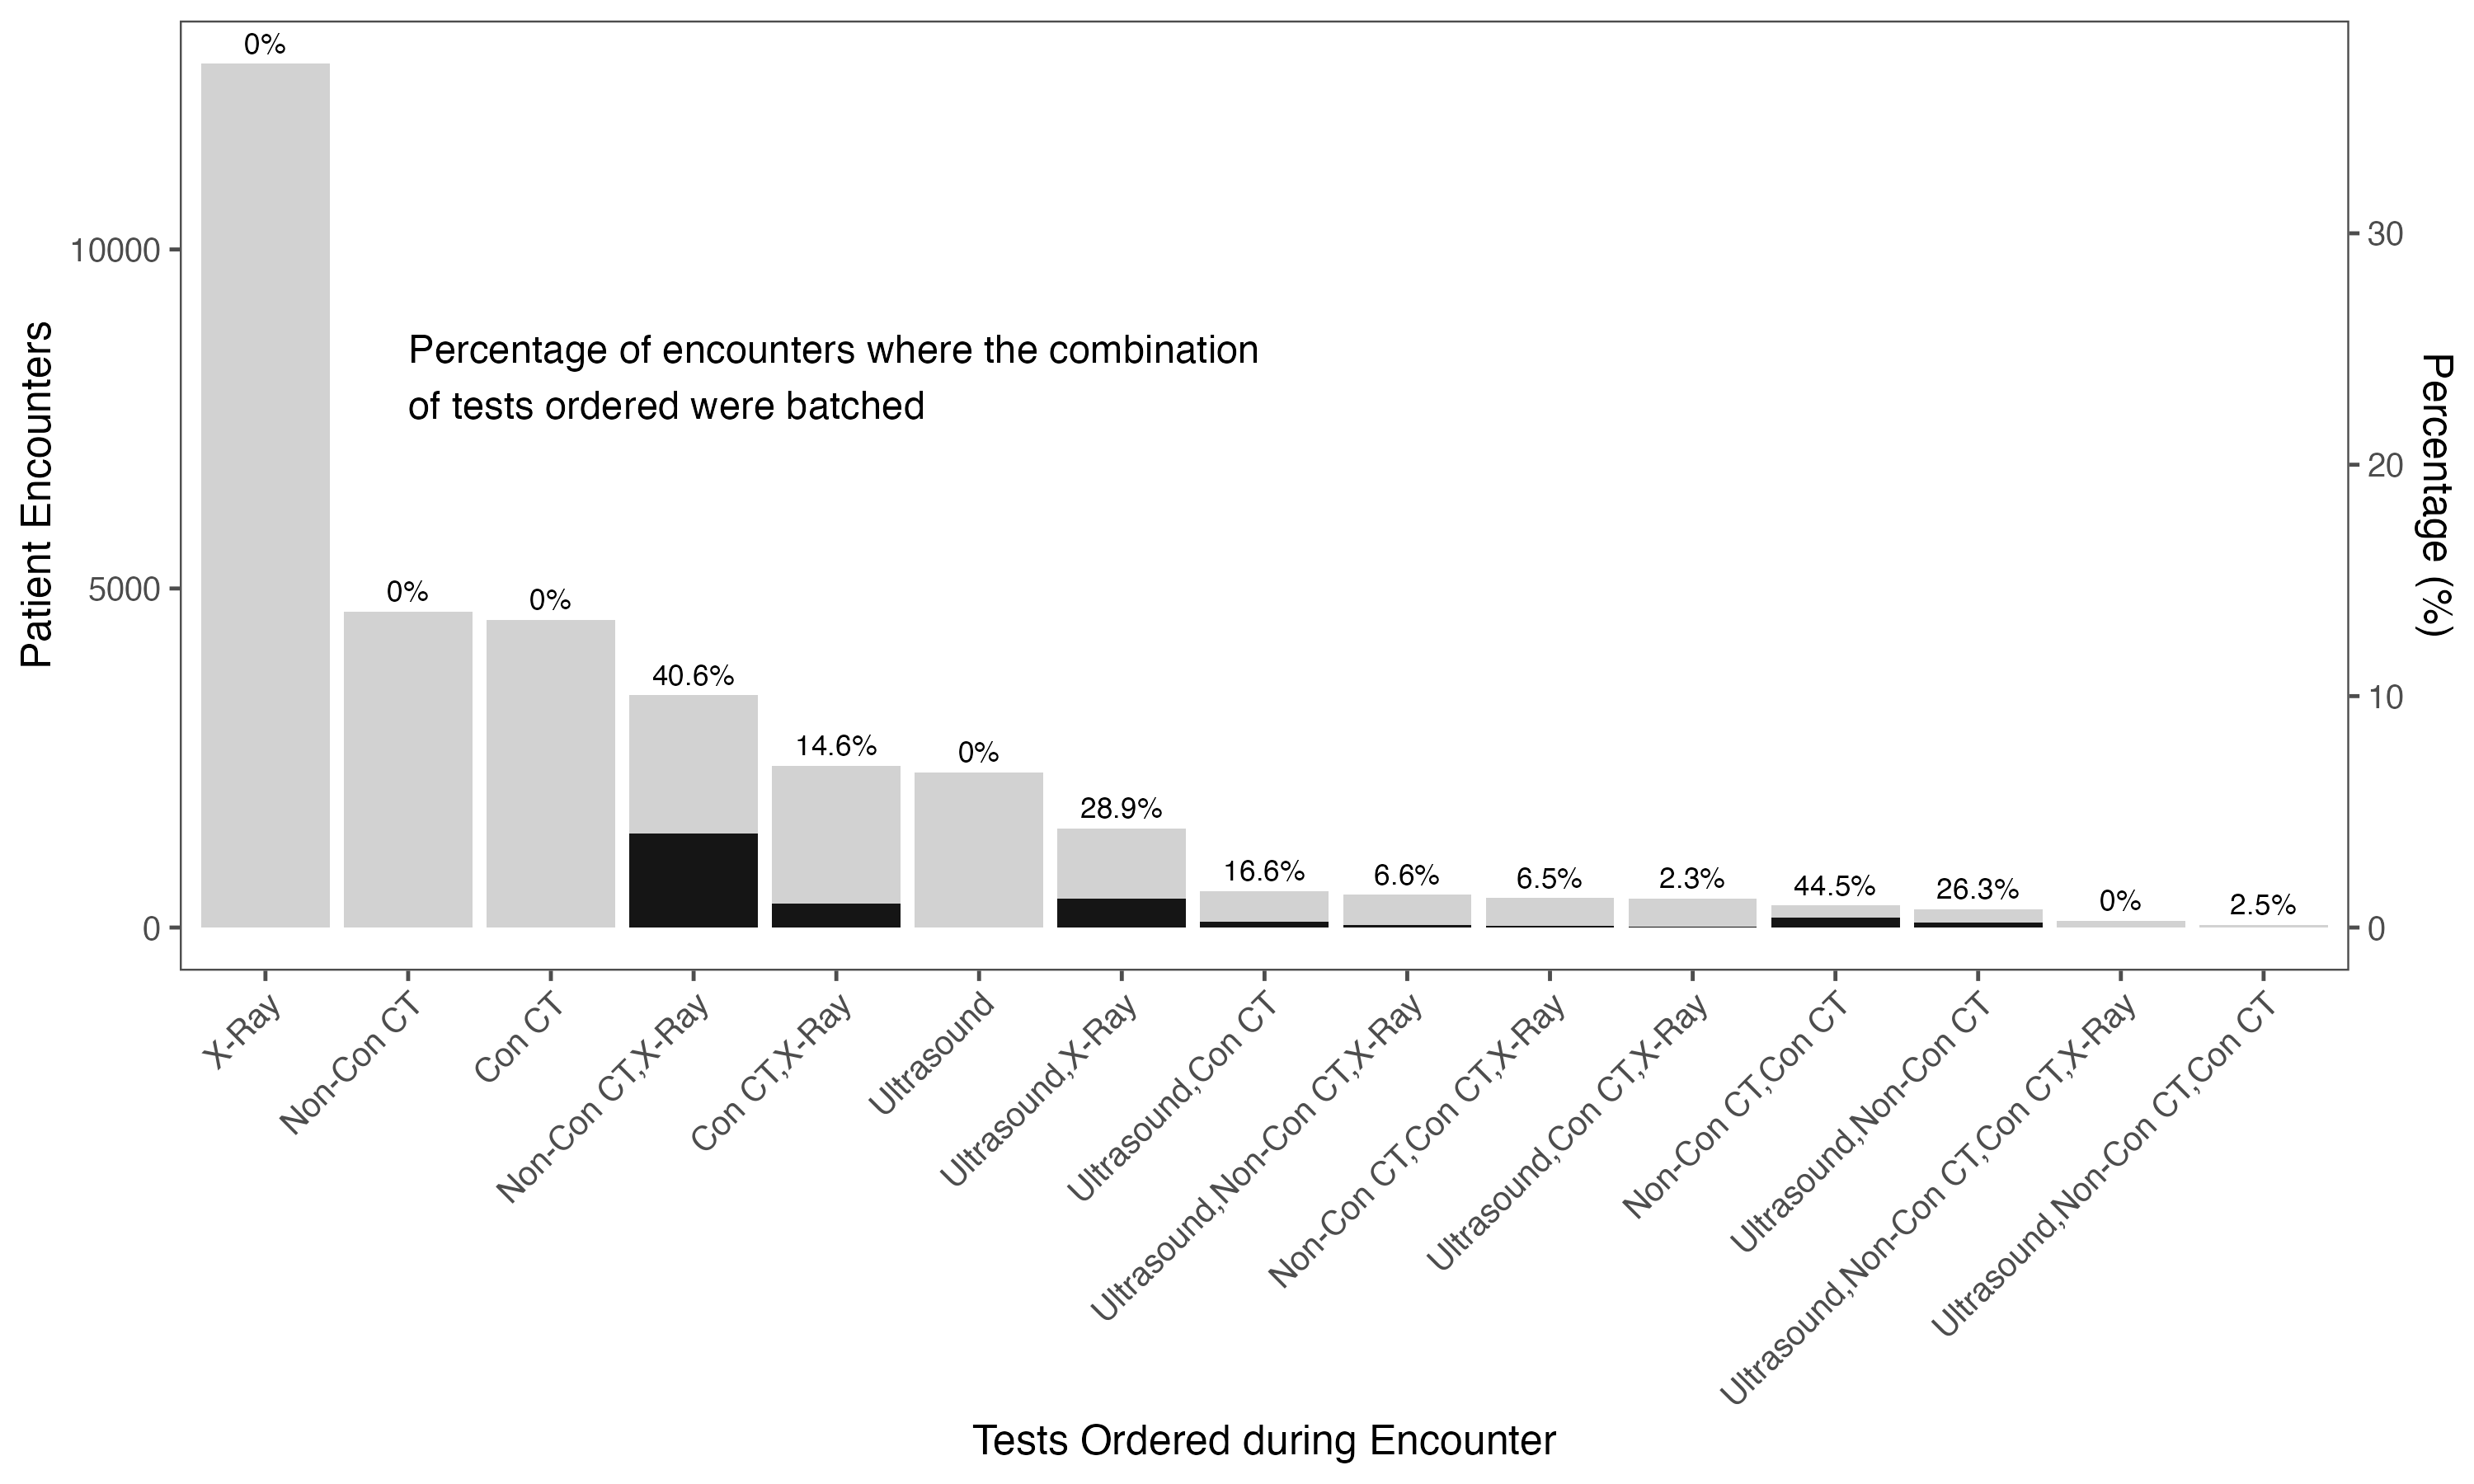
\includegraphics[width=0.8\textwidth]{../outputs/figures/combined_tests.png}    
\label{fig:consort}    
\begin{tablenotes}
\small
\item \textit{Notes:} Figure shows frequency of different imaging test combinations and the proportion of each combination that was batch-ordered (tests ordered within 5 minutes). Sample restricted to encounters where at least one imaging test was ordered.
\end{tablenotes}
\end{threeparttable}
\end{figure}

This figure reveals key insights for interpreting Panel B:

First, X-rays are by far the most common test (appearing in 67\% of encounters alone and in most combinations), yet they are batched at dramatically different rates depending on context. X-ray alone is never batched (by definition—batching requires 2+ tests), but X-ray combined with non-contrast CT is batched 40.6\% of the time, while X-ray with contrast CT is batched only 14.6\% of the time. 

Second, our IV estimates in Panel B identify which specific tests physicians add when they engage in discretionary batching. The coefficients represent the causal effect of the batching decision on test utilization patterns, revealing how physicians construct comprehensive workups when they choose to batch rather than sequence tests.

\textbf{Revised Table 4 with enhanced controls:}

Our revised Table 4 incorporates the expanded control set we developed in response to all three reviewers' concerns about our original specification:


\begin{table}[H]
\centering
\caption*{Table 4     IV Results: Effect of Batching Tests on Patient Outcomes}
\label{tab:results_table}
\begin{threeparttable}
\begin{tabular}{lccccc}
\toprule
& Sequenced & \multicolumn{2}{c}{\underline{OLS results}} & \multicolumn{2}{c}{\underline{2SLS results}} \\
& mean & (2) & (3) & (4) & (5) \\
\midrule
\multicolumn{6}{l}{\textit{Panel A. Primary Outcomes}} \\[0.5em]
Log time to disposition & 5.237 & $0.084^{***}$ & $0.072^{***}$ & $0.618$ & $0.630$ \\
& (0.499) & (0.014) & (0.013) & (0.456) & (0.460) \\[0.5em]
Log LOS & 5.490 & $0.107^{***}$ & $0.073^{***}$ & $0.679^{\dagger}$ & $0.580$ \\
& (0.456) & (0.013) & (0.012) & (0.341) & (0.341) \\[0.5em]
Number of distinct imaging tests & 1.334 & $0.839^{***}$ & $0.802^{***}$ & $1.360^{***}$ & $1.214^{***}$ \\
& (0.571) & (0.017) & (0.019) & (0.199) & (0.196) \\[0.5em]
72hr return with admission & 0.012 & -0.001 & 0.000 & -0.011 & -0.012 \\
& (0.110) & (0.002) & (0.003) & (0.021) & (0.025) \\[0.5em]

\multicolumn{6}{l}{\textit{Panel B. Test Types}} \\[0.5em]
Ultrasound & 0.171 & $0.072^{***}$ & $0.117^{***}$ & 0.162 & 0.089 \\
& (0.376) & (0.016) & (0.014) & (0.101) & (0.082) \\[0.5em]
CT with contrast & 0.187 & 0.029 & $0.051^{**}$ & $0.168^{\dagger}$ & 0.085 \\
& (0.390) & (0.015) & (0.014) & (0.071) & (0.069) \\[0.5em]
CT without contrast & 0.400 & $0.383^{***}$ & $0.279^{***}$ & 0.105 & 0.067 \\
& (0.490) & (0.015) & (0.012) & (0.137) & (0.138) \\[0.5em]
X-ray & 0.576 & $0.354^{***}$ & $0.356^{***}$ & $0.925^{***}$ & $0.972^{**}$ \\
& (0.494) & (0.012) & (0.012) & (0.220) & (0.260) \\[0.5em]

\multicolumn{6}{l}{\textit{Panel C. Disposition}} \\[0.5em]
Admission & 0.279 & $0.035^{*}$ & $0.027^{**}$ & $0.397^{***}$ & $0.392^{***}$ \\
& (0.449) & (0.013) & (0.009) & (0.088) & (0.071) \\[0.5em]
\midrule
Time FE & --- & Yes & Yes & Yes & Yes \\
Baseline controls & --- & No & Yes & No & Yes \\
Observations & 11,651 & 11,651 & 11,651 & 11,651 & 11,651 \\
\bottomrule
\end{tabular}
\begin{tablenotes}
\footnotesize
\item \textit{Notes:} This table reports the estimated coefficients of both OLS and 2SLS regressions of the effect of batching on patient outcomes. The OLS columns include no controls (column 2) and baseline controls (column 3). The 2SLS columns include no controls (column 4) and baseline controls (column 5). Standard errors are clustered at the physician level.
\item $^{\dagger} p < 0.10$, $^{*} p < 0.05$, $^{**} p < 0.01$, $^{***} p < 0.001$.
\end{tablenotes}
\end{threeparttable}
\end{table}

Focusing on Column 5 (our primary specification with full controls), Panel B shows:

- X-rays increase by 97.2 percentage points (0.972, p<0.01) — nearly every discretionary batch includes an X-ray, consistent with X-rays being quick additions to imaging workups

- Other imaging shows smaller, non-significant effects: CT with contrast (8.5pp), CT without contrast (6.7pp), Ultrasound (8.9pp) are all statistically insignificant at the 5\% level

This pattern makes clinical sense: when physicians choose to batch, they nearly universally add a simple X-ray but are more selective about expensive advanced imaging. The IV approach ensures we identify the causal effect of the batching strategy rather than simply correlating test types with batching decisions.

\textbf{2. Explaining the admission effect magnitude:}

The reviewer correctly notes that the 39.2 percentage point admission increase (Column 5) is substantial. In our original submission, this effect was even larger, raising valid concerns about whether the instrument might capture physician admission propensity independent of imaging decisions.

To address this concern, we examined whether controlling for physician admission tendency—constructed using the same leave-one-out residualization approach as our batch tendency instrument—would attenuate the effect. We present these results in Appendix D:

\begin{table}[h]
\centering
\caption*{Sensitivity to Admission Tendency Control}
\begin{threeparttable}
\begin{tabular}{lcc}
\toprule
& Column 5 & Model 5 \\
& (Primary Spec) & (+Admit Tendency) \\
\midrule
Admission effect & 0.392*** & 0.216*** \\
& (0.071) & (0.056) \\
Number of imaging tests & 1.214*** & 1.063*** \\
& (0.196) & (0.197) \\
\midrule
Controls & Full & Full + Admit Tendency \\
First-stage F-stat & 276.8 & 153.1 \\
\bottomrule
\end{tabular}
\begin{tablenotes}
\footnotesize
\item \textit{Notes:} Column 5 shows our primary specification from Table 4 with patient characteristics, physician characteristics, laboratory ordering, and hours into shift. Model 5 adds physician admission tendency (leave-one-out residualized propensity to admit). Standard errors clustered at the physician level. *** p<0.001.
\end{tablenotes}
\end{threeparttable}
\end{table}

The admission effect attenuates from 39.2pp to 21.6pp when controlling for admission tendency, suggesting that some portion reflects correlated physician behaviors. However, we note three important qualifications:

First, admission may lie on the causal pathway from batching (batching → more tests → more findings → admission decision), making admission tendency a "bad control" that absorbs treatment effects rather than isolating confounds. The attenuation could reflect controlling away the mechanism rather than removing bias.

Second, even in this conservative specification, substantial effects persist: a 21.6pp admission increase, demonstrating that the imaging-admission pathway remains economically and statistically significant (p<0.001).

Third, imaging volume effects remain large (1.063 tests, p<0.001) even when controlling for admission tendency, confirming that discretionary batching genuinely increases diagnostic intensity. For marginal patients whose disposition is uncertain, 1.2 additional imaging tests provide more opportunities for incidental findings that push physicians toward defensive admission decisions.

We interpret these results as follows: Discretionary batching creates a cascade where the decision to order comprehensive imaging upfront leads to (1) significantly more tests performed (1.214 additional tests), particularly X-rays, and (2) substantially higher admission rates. 

While some portion of the admission effect may reflect correlated physician tendencies toward both batching and admission, the persistence of large effects even in conservative specifications controlling for admission tendency (21.6pp, p<0.001) supports that the imaging pathway represents a significant mechanism. The additional diagnostic information from discretionary batching—notably the near-universal addition of X-rays—provides more opportunities for findings (including incidental ones) that influence disposition decisions.

We acknowledge this interpretation in our revised limitations section (Section 4.8), noting that the admission effects likely reflect both the causal imaging pathway and some correlated physician practice patterns. We emphasize that the imaging volume effects provide clear evidence of the resource utilization consequences of discretionary batching.

\textbf{Manuscript changes:}

\begin{enumerate}
\item Updated Table 4 to reflect enhanced specification with full controls
\item Added to Appendix D showing sensitivity to admission tendency control
\item Revised discussion of admission effects (Section 4.2) to acknowledge potential for correlated physician behaviors while emphasizing the imaging volume mechanism
\item Enhanced limitations section (Section 4.8) discussing the causal pathway interpretation
\end{enumerate}

We thank the reviewer for pushing us to clarify these important interpretive issues, which have led to a more nuanced and defensible presentation of our findings.
\color{black}

\begin{quote2}
\textbf{R3 Wrote (Major concern -  Model selection):}  

\noindent``The authors use a linear model for all outcome variables, regardless of whether the outcomes are binary, count, or continuous. Are the results robust to more appropriate model specifications that better align with the nature of each outcome variable?"
\end{quote2}



\noindent\textbf{Response:} \color{blue}We thank the reviewer for this methodological question. The reviewer correctly notes that our outcomes include binary (admission, 72-hour return), count (number of tests), and continuous (log time) variables. We use linear models throughout our 2SLS analysis, which is standard practice in the causal inference literature for important econometric reasons we explain below.

\textbf{Why linear models in IV settings:}

While nonlinear models (logit/probit for binary outcomes, Poisson for counts) seem more appropriate for the outcome distributions, using them in instrumental variables settings creates fundamental econometric problems. The key issue is what \cite{hausman1975, Hausman1978} termed the ``forbidden regression."

When using a nonlinear first stage (e.g., probit for our binary batching variable), substituting the fitted values $\hat{d}_i$ into any second stage creates:

$$y_i = \beta_0 + \beta X_i + \gamma \hat{d}_i + [\epsilon_i + \gamma(d_i - \hat{d}_i)]$$

This fails because with a nonlinear first stage, the residuals $(d_i - \hat{d}_i)$ are correlated with $\hat{d}_i$ even asymptotically, unless the first-stage functional form is exactly correct—an untestable assumption. Consistency of 2SLS estimates does not depend on correct specification of the first-stage conditional expectation function, but this robustness is lost with nonlinear first stages (\cite{angrist2009mostly}).

Using nonlinear models in the second stage is even more problematic. The linear 2SLS estimator provides a well-defined Local Average Treatment Effect (LATE) for compliers. Nonlinear second-stage models would require strong assumptions about the entire joint distribution of errors and lack the LATE interpretation. Combining the nonlinear first and second stages compounds these problems.

The linear probability model in 2SLS, while potentially producing predictions outside [0,1] for individual observations, yields consistent estimates of the average marginal effect for compliers—exactly the parameter of policy interest in our quasi-experimental setting.

\textbf{Robustness check—OLS functional form comparison:}

Nevertheless, to address the reviewer's concern about functional form, we verified that OLS estimates (which do not face the forbidden regression problem) using nonlinear models show qualitatively similar patterns to our linear OLS results. We present these comparisons in Appendix D (and here):

\begin{table}[H]
\centering
\caption*{Robustness: Linear vs. Nonlinear Models (OLS Only)}
\begin{threeparttable}
\begin{tabular}{lccc}
\toprule
& Linear OLS & Nonlinear & \\
& (Table 4, Col 3) & Model (AME) & Difference \\
\midrule
\textit{Binary Outcomes} \\
Admission & 0.027*** & 0.024*** & -0.003 \\
& (0.009) & (0.008) & (11\%) \\
72hr return w/ admit & -0.000 & -0.000 & 0.000 \\
& (0.003) & (0.003) & --- \\
\midrule
\textit{Count Outcome} \\
Number of imaging tests & 0.802*** & 0.670*** & -0.132 \\
& (0.019) & (0.017) & (16\%) \\
\bottomrule
\end{tabular}
\begin{tablenotes}
\footnotesize
\item \textit{Notes:} Linear OLS results from Table 4, Column 3 (baseline controls). Nonlinear models use logit for binary outcomes and negative binomial for count outcomes. Average marginal effects (AME) are reported for nonlinear models to enable direct comparison with linear coefficients. All models include full controls: patient characteristics, physician characteristics, laboratory ordering, hours into shift, and fixed effects. Standard errors clustered at the physician level. We do not present nonlinear 2SLS results due to the econometric issues discussed above. *** p<0.001.
\end{tablenotes}
\end{threeparttable}
\end{table}

The average marginal effects from nonlinear OLS models are very similar to the linear OLS coefficients:

- Admission: 2.7pp (linear) vs. 2.4pp (logit AME) — 11\% difference

- 72-hour return: Effectively zero in both specifications  

- Number of tests: 0.80 (linear) vs. 0.67 (negative binomial AME) — 16\% difference

These differences are economically small and do not change any substantive conclusions. Since our 2SLS estimates are larger than OLS (as expected given endogeneity correction), and the OLS functional form is robust to nonlinear alternatives, this provides confidence that our linear 2SLS approach yields reliable causal estimates without introducing the biases inherent in nonlinear IV specifications.

\textbf{Manuscript changes:}

We have added a discussion in Section 3.4 (Empirical Specification) explaining our choice of linear models in the IV framework, with reference to the econometric literature on the forbidden regression problem. We have also added Appendix D, which shows the OLS robustness check with nonlinear models.

We appreciate the reviewer raising this methodological point, as it allows us to clarify why the linear model is not just convenient but econometrically preferable in IV settings, while also demonstrating that functional form does not drive our OLS results.

\color{black}


\begin{quote2}
\textbf{R3 Wrote (Major concern -  Sample selection):}  

\noindent``The final sample for the primary data includes less than 25\% of all ED encounters. Could the authors provide more details regarding the sample selection process, including the exact number of observations excluded with each criterion? 

Given such a substantial reduction in sample size, it is crucial for the authors to compare the excluded and included encounters to ensure that the observed effects are not limited to a small, non-representative subsample of ED visits."
\end{quote2}


\noindent\textbf{Response:} \color{blue}We thank the reviewer for requesting greater transparency about sample selection. We address this concern by (1) providing a detailed CONSORT flow diagram showing exact exclusion counts, (2) comparing characteristics of excluded versus included encounters, and (3) explaining why our focused sample strengthens rather than limits our contribution.

\textbf{1. CONSORT flow diagram:}

Figure A2 (Appendix) shows the complete sample selection process:

\begin{figure}[ht]
\centering
\begin{threeparttable}
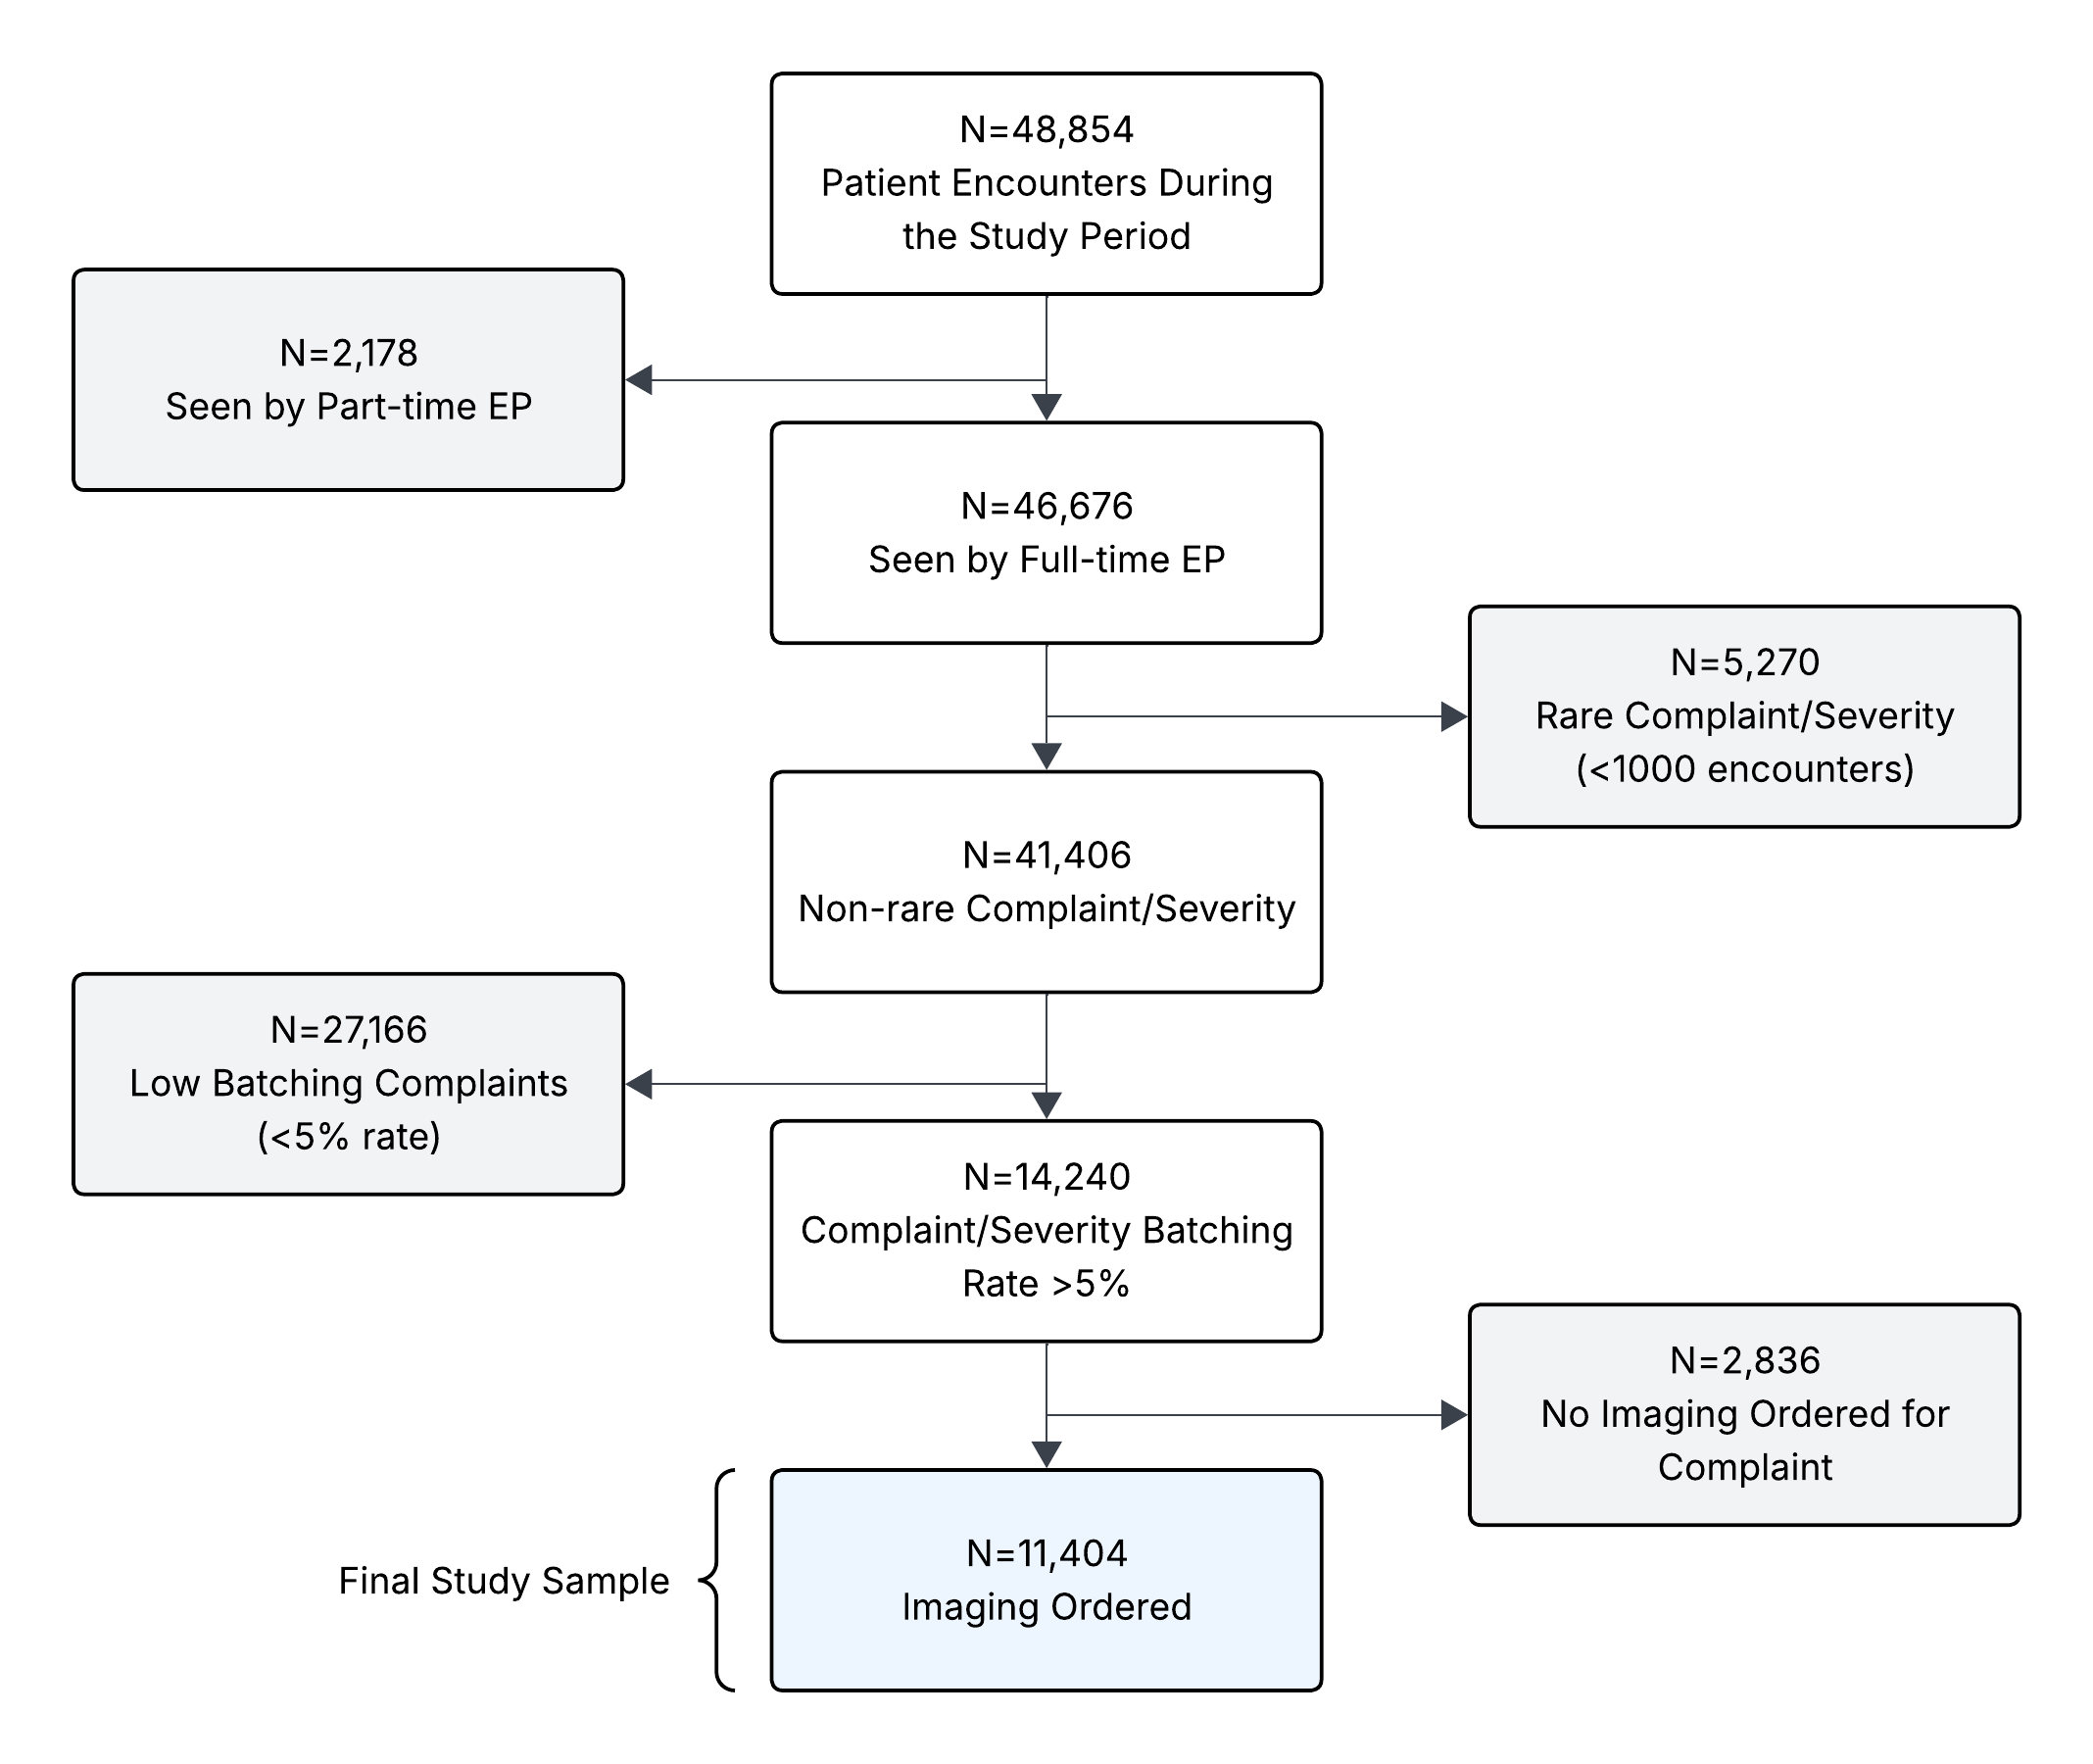
\includegraphics[width=0.8\textwidth]{../outputs/figures/CONSORT.png}    
\caption{CONSORT Flow Diagram for Sample Selection}    
\label{fig:consort}    
\begin{tablenotes}
\small
\item \textit{Notes:} Sample selection for Mayo Clinic ED encounters (October 2018 - December 2019). Starting with 48,854 encounters, we apply sequential exclusion criteria to arrive at our analytical sample of 11,404 encounters. Rare complaints have fewer than 1,000 total encounters. Low-batching complaints have batching rates below 5\%.
\end{tablenotes}
\end{threeparttable}
\end{figure}

Starting with 48,854 encounters of adult patients, we exclude: (1) encounters with non-full time providers, (2) rare complaints (<1,000 encounters), (3) complaints where batching occurs <5\% of the time, and (4) complaints that do not involve any imaging. This yields our analytical sample of 11,651 encounters (27.4\%).

The table below (now included in Appendix A) compares patient characteristics and outcomes between excluded and included encounters:

\begin{table}[H]
\centering
\caption*{Comparison of Excluded vs. Included Encounters}
\begin{threeparttable}
\begin{tabular}{lccc}
\toprule
& Excluded & Included & \\
& Encounters & (Analytical Sample) & p-value \\
\midrule
\textit{Demographics} \\
Age (years) & 57.5 (19.6) & 62.9 (18.3) & <0.001*** \\
\midrule
\textit{Acuity} \\
ESI Level (mean) & 2.87 (0.64) & 2.52 (0.59) & <0.001*** \\
\midrule
\textit{Vital Signs} \\
Tachycardic (\%) & 18.8 & 20.1 & 0.001*** \\
Tachypneic (\%) & 9.1 & 9.2 & 0.567 \\
Febrile (\%) & 1.4 & 4.6 & <0.001*** \\
Hypotensive (\%) & 1.2 & 2.3 & <0.001*** \\
\midrule
\textit{Outcomes} \\
ED LOS (minutes) & 238.3 (135.0) & 272.0 (133.5) & <0.001*** \\
Admission rate (\%) & 17.0 & 28.4 & <0.001*** \\
\midrule
N & 37,450 & 11,651 & \\
\% of total sample & 72.5\% & 27.4\% & \\
\bottomrule
\end{tabular}
\begin{tablenotes}
\footnotesize
\item \textit{Notes:} Comparison of patient characteristics and outcomes between excluded encounters (n=37,450) and analytical sample (n=11,651). Standard deviations in parentheses for continuous variables. ESI (Emergency Severity Index) ranges from 1 (highest acuity) to 5 (lowest acuity). P-values from two-sample t-tests for continuous variables and proportion tests for binary variables. *** p<0.001.
\end{tablenotes}
\end{threeparttable}
\end{table}

The analytical sample differs from excluded encounters in clinically meaningful and expected ways. Included patients are older (62.9 vs. 57.5 years), higher acuity (ESI 2.52 vs. 2.87, where lower numbers indicate greater severity), and more likely to present with concerning vital signs (febrile: 4.6\% vs. 1.4\%, hypotensive: 2.3\% vs. 1.2\%). Consequently, they experience longer ED stays (272 vs. 238 minutes) and higher admission rates (28.4\% vs. 17.0\%).

These differences strengthen rather than limit our contribution. The analytical sample comprises precisely the population where imaging decisions matter most: moderate-to-high acuity patients presenting with complaints commonly requiring diagnostic workups. These are the encounters where physicians face genuine uncertainty about optimal testing strategy and where efficiency gains from improved ordering practices would be most impactful. Excluded encounters—primarily low-acuity visits where imaging is rarely needed—represent settings where batching decisions are either clinically inappropriate or operationally irrelevant.

Importantly, these differences reflect an appropriate sample definition rather than selection bias. Mayo Clinic's random assignment mechanism ensures physicians see the full spectrum of acuity and complaints. Our analytical sample focuses on encounters where the batching decision is both consequential and discretionary—precisely the population where our LATE provides actionable policy guidance.

Our sample restrictions serve two purposes, both standard in the judges design literature:

First, instrumental variable identification requires variation. Our IV approach needs sufficient batching variation to generate a strong first stage. Including complaints where batching rarely occurs would create weak instrument problems, yielding imprecise and uninformative estimates of the LATE.

Second, our research question concerns discretionary decisions. We identify the Local Average Treatment Effect for patients whose testing strategy depends on physician preference rather than clinical necessity. This is precisely the population of policy interest: encounters where multiple imaging pathways are clinically plausible and efficiency tradeoffs matter. Our sample includes complaints commonly requiring imaging (Neurological Issues, Abdominal Pain, Chest Pain, Falls/Trauma, Dizziness/Syncope, Extremity Complaints, Constitutional Symptoms) where physicians make consequential ordering decisions.

Importantly, random assignment ensures these exclusions do not introduce selection bias. Physicians receive all complaint types through Mayo Clinic's rotational system. We focus our analysis on complaints where their batching decisions vary meaningfully. We verify balance by: (1) computing batch tendency using physicians' behavior across ALL encounters before exclusions, and (2) confirming patient characteristics remain balanced within our analytical sample (Figure 2).

While our results apply to the 25\% of ED visits requiring imaging workups, this represents the clinically and operationally relevant population. Batching cannot affect outcomes for complaints that never require imaging, and for complaints that always require multiple tests, the decision is clinically determined rather than discretionary. Our focused approach identifies the precise effects where physician practice style influences operations—the margin where ED management interventions can meaningfully improve efficiency.

\textbf{Manuscript changes:}

\begin{enumerate}
\item Added detailed CONSORT diagram (Appendix A)
\item Added comparison of excluded vs. included encounters (Appendix A)
\item Revised Section 3.2 to clarify sample selection rationale with appropriate citations
\item Added discussion of generalizability in Section 5.3 (Limitations)
\end{enumerate}

We appreciate the reviewer's attention to this issue, which has led us to provide greater transparency about our sample construction and its implications for interpreting our findings.

\color{black}



\begin{quote2}
\textbf{R3 Wrote (Major concern -  Variable selection):}  

\noindent``To estimate the impact of batch ordering on productivity, the authors focus on LOS and time to disposition. However, the most relevant outcome for assessing physician practice is treatment time, defined as the period from the start of assessment to disposition. I recommend that the authors consider this metric, as it excludes both the waiting time before assessment and the boarding time after disposition.

The authors use a 72-hour ED revisit leading to hospital admission as an indicator of care quality. While this is conceptually a valid measure, it is more common in both the operations management and medical literature to use ED revisit—regardless of admission status—as an indicator of adverse outcomes. Are the results robust to this alternative measure of quality? From the estimation perspective, this measure should be a better choice given the scarcity of ED revisits leading to hospital admission.

On a related note, how do the authors measure 72-hour ED revisit for patients who were admitted to the hospital during the focal visit?"
\end{quote2}

\noindent\textbf{Response:} \color{blue}We thank the reviewer for these important suggestions about outcome measures. We address each in turn:

\textbf{1. Treatment time:} 

We appreciate the reviewer highlighting treatment time as a valuable measure that excludes both waiting room delays and post-disposition boarding. While our primary time-to-disposition measure already excludes boarding time and our controls for capacity level and time fixed effects account for waiting room variation, we agree that treatment time provides a cleaner measure of physician productivity. 

We have therefore added this analysis using treatment time (defined as the time from the first physician contact to the disposition decision). The results, shown in the table below (now in Appendix D), demonstrate that our findings are robust to this alternative specification:

\begin{table}[H]
\centering
\caption*{Robustness: Alternative Time Measures}
\begin{threeparttable}
\begin{tabular}{lcc}
\toprule 
& Log Time to & Log Treatment \\ 
& Disposition & Time \\ 
\midrule
2SLS Coefficient & 0.630 & 0.664 \\
(SE) & (0.460) & (0.485) \\
p-value & 0.172 & 0.171 \\
\midrule
Percentage Increase & 88\% & 94\% \\
Baseline mean (sequenced) & 5.24 & 5.18 \\
\midrule
Controls & Full & Full \\
Observations & 11,651 & 11,651 \\
\bottomrule
\end{tabular}
\begin{tablenotes}
\footnotesize
\item \textit{Notes:} 2SLS estimates with batch tendency as instrument. Full controls include patient characteristics, physician characteristics, laboratory ordering, hours into shift, and temporal fixed effects. Time to disposition excludes post-decision boarding. Treatment time excludes both waiting time before assessment and post-decision boarding. Standard errors clustered at the physician level. Percentage effects calculated as $[exp(\beta)-1]\times 100$.
\end{tablenotes}
\end{threeparttable}
\end{table}

The similar magnitude and pattern of effects (94\% vs. 88\% increases, both p>0.10) confirms that batch ordering shows similar point estimates for delays in physician productivity regardless of how we measure processing time. We thank the reviewer for this suggestion, which strengthens our analysis by demonstrating robustness to alternative time measures.

\textbf{2. 72-hour revisit measures:} 

The reviewer correctly notes that any 72-hour ED revisit is more commonly used than revisit-with-admission. We initially focused on 72-hour returns requiring admission based on guidance from our physician coauthors (including emergency physicians at both study sites), who indicated this measure better captures true quality failures. Some ED revisits are planned or expected—patients may be instructed to return for wound checks, suture removal, or if symptoms persist after initial treatment. Returns requiring admission, however, are more likely to indicate missed diagnoses or inadequate initial treatment.

Nevertheless, we acknowledge the reviewer's point about statistical power and comparability with prior literature. We therefore re-estimated our models using any 72-hour ED revisit as the outcome:

\begin{table}[H]
\centering
\caption*{Robustness: Alternative Quality Measures}
\begin{threeparttable}
\begin{tabular}{lcc}
\toprule 
& 72hr Return & Any 72hr \\ 
& with Admission & Return \\ 
\midrule
2SLS Coefficient & -0.012 & -0.051 \\
(SE) & (0.025) & (0.044) \\
p-value & 0.648 & 0.250 \\
\midrule
Baseline mean (sequenced) & 1.2\% & 3.0\% \\
\midrule
Controls & Full & Full \\
Observations & 11,651 & 11,651 \\
\bottomrule
\end{tabular}
\begin{tablenotes}
\footnotesize
\item \textit{Notes:} 2SLS estimates with batch tendency as an instrument. Full controls include patient characteristics, physician characteristics, laboratory ordering, hours into shift, and temporal fixed effects. Standard errors clustered at the physician level.
\end{tablenotes}
\end{threeparttable}
\end{table}

The results remain statistically insignificant for both measures (p=0.648 and p=0.250), with point estimates suggesting no adverse quality effects. If anything, both measures show negative point estimates, suggesting batch ordering does not increase (and may slightly decrease) return rates, though the effects are imprecise and statistically indistinguishable from zero. We have added this robustness check to Appendix D.

\textbf{3. Measurement for admitted patients:}

For patients admitted during their index visit, the 72-hour window begins at hospital discharge, not ED departure. Admitted patients cannot revisit the ED while hospitalized. This standard approach ensures fair comparison across all patients regardless of initial disposition. We have clarified this measurement approach in Section 3.2.2.

\textbf{Manuscript changes:}

\begin{enumerate}
\item Added treatment time analysis (Appendix D)
\item Added any 72-hour return analysis (Appendix D)
\item Clarified 72-hour return measurement for admitted patients (Section 3.2.2)
\end{enumerate}

We appreciate the reviewer's suggestions, which allow us to demonstrate that our findings are robust to alternative outcome specifications while maintaining our focus on the most clinically meaningful quality measure.

\color{black}

\begin{quote2}
\textbf{R3 Wrote (Major concern -  Heterogeneity analysis):}  

\noindent``The authors correctly discuss the trade-offs between the advantages and disadvantages of batch ordering diagnostic tests compared to sequential test ordering. However, the paper subsequently focuses primarily on the disadvantages of batch ordering. While it is important to quantify the overall net benefit or cost of ordering diagnostic tests in advance, I believe the paper would provide more comprehensive insights for practice if it also identified the conditions under which one strategy outperforms the other. Specifically, are there certain chief complaints for which a batching strategy leads to better outcomes? I would expect this to be the case for more complex chief complaints that generally require a greater number of diagnostic tests.

In addition, is there evidence of heterogeneity in the effect or magnitude of the impact of batch ordering across conditions where batching is more common? Understanding such variation could help tailor diagnostic strategies to different clinical scenarios."
\end{quote2}

\noindent\textbf{Response:} \color{blue}We thank the reviewer for this excellent suggestion to explore heterogeneity in batching effects. We conducted a comprehensive analysis examining effects across our seven chief complaint categories, which vary substantially in both clinical complexity and batching prevalence (ranging from 7\% for fevers to 24\% for polytrauma). 

Figure 4 presents this heterogeneity analysis, with complaints ordered by batching rate. The color gradient illustrates variation in batching prevalence, from red (high-batching complaints) to blue (low-batching complaints).

\begin{figure}[H]
\centering
\caption*{Heterogeneity in Batch Ordering Effects by Chief Complaint}
\begin{threeparttable}
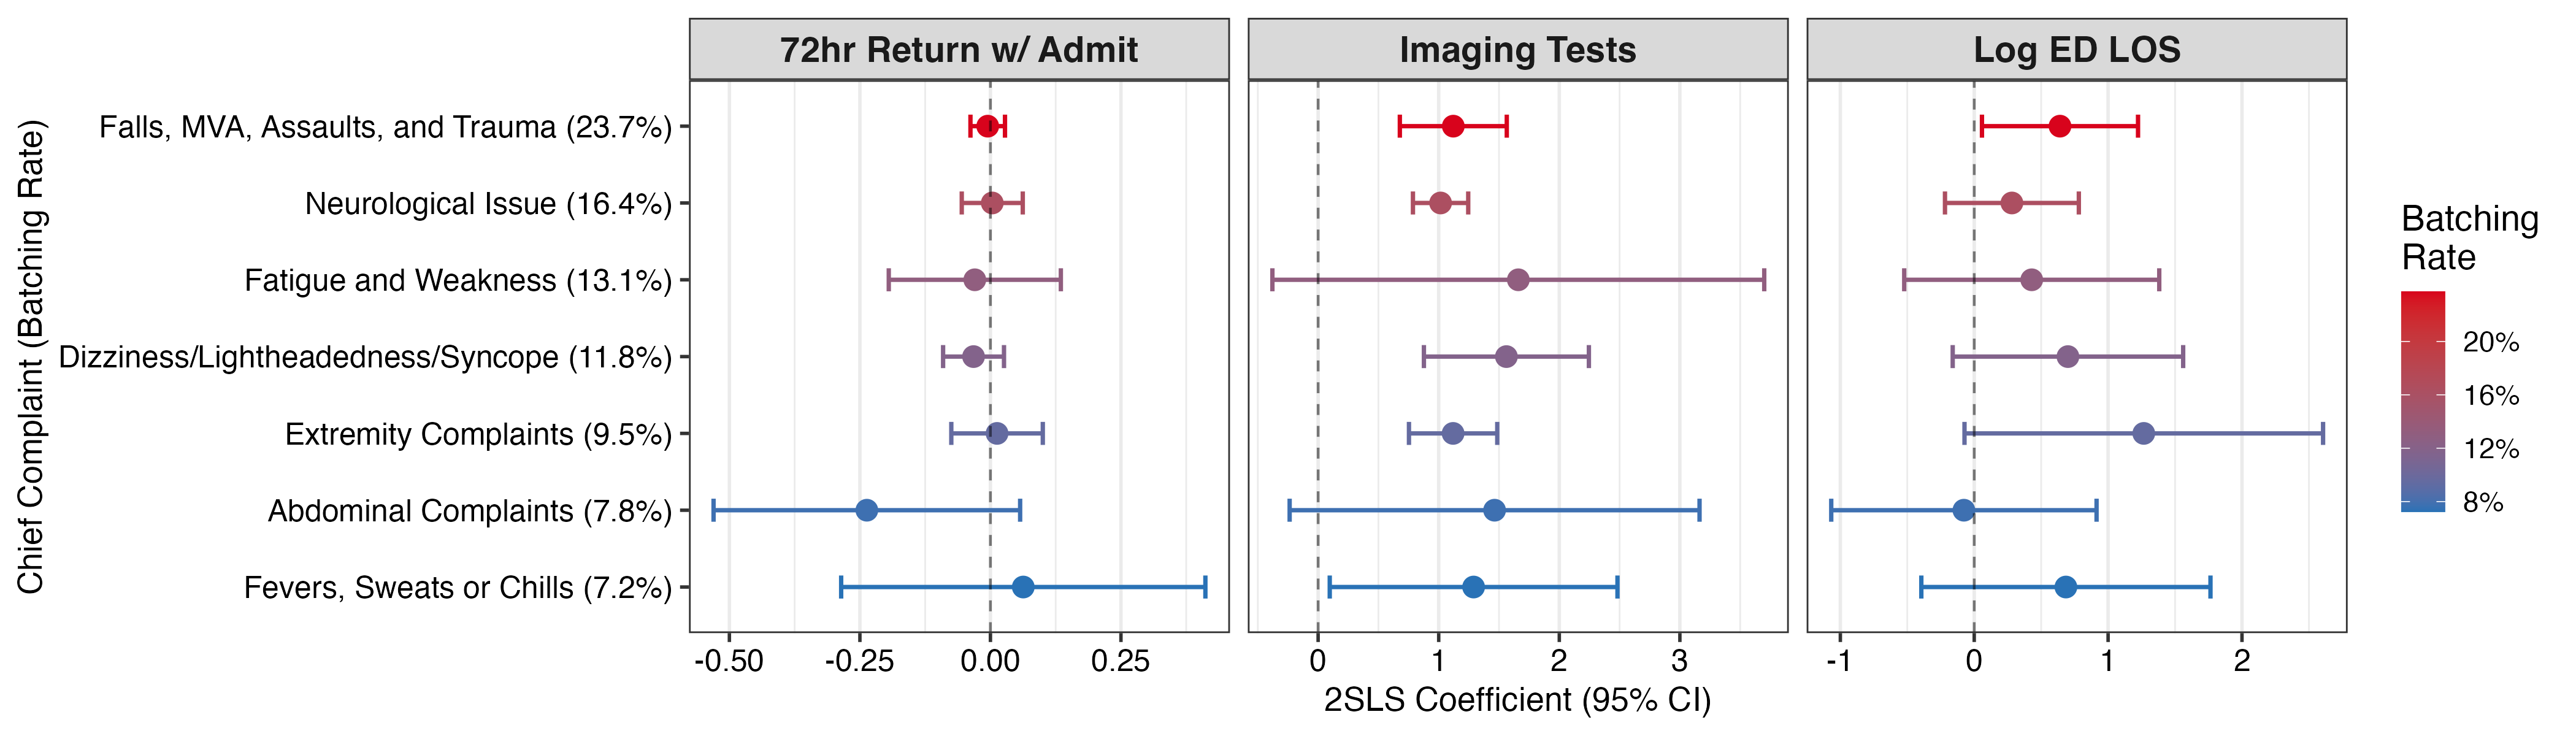
\includegraphics[width=\textwidth]{../outputs/figures/heterogeneity_by_complaint.png}    
\begin{tablenotes}
\small
\item \textit{Notes:} Each panel shows 2SLS estimates of batching effects for different chief complaints, ordered by batching rate (shown in parentheses). Point colors indicate batching prevalence. Error bars show 95\% confidence intervals with standard errors clustered at the physician level. All models include full controls.
\end{tablenotes}
\end{threeparttable}
\end{figure}

We frame this as an exploratory analysis given multiple hypothesis testing concerns across seven categories and three outcomes. Rather than emphasizing statistical significance in subgroups, we focus on whether any clinical scenario shows qualitatively different patterns in direction or magnitude.

The reviewer's intuition that batching might benefit complex complaints is reasonable, but our analysis reveals no such pattern. Imaging volume effects are consistently positive across all complaint types (ranging from 1.0 to 1.7 additional tests), with five of seven showing statistical significance despite reduced sample sizes. Critically, Falls/Trauma/MVA—our most complex category with the highest batching rate (23.7\%)—shows a 1.12 test increase (p<0.001). This challenges the clinical intuition that "comprehensive upfront imaging" improves care for complex polytrauma presentations.

Time effects show no evidence of efficiency gains in any category. Point estimates cluster around our main results, with none suggesting time savings. The Falls/Trauma category shows a positive coefficient of 0.64, suggesting delays rather than improvements for the most complex cases, where batching is most common. Quality effects remain close to zero across all complaints (point estimates from -0.24 to +0.06, all p>0.10), indicating that batching neither improves nor harms outcomes regardless of clinical complexity.

The consistency across complaint types is striking. Despite substantial variation in complexity and batching prevalence, the fundamental pattern persists: increased imaging without measurable time savings or quality improvements. This suggests that recommendations against discretionary batching apply broadly, and that even for complex presentations, sequential ordering allows physicians to target imaging based on initial findings rather than preemptively ordering tests that may prove unnecessary.

\textbf{Manuscript changes:}

We have added Section 4.4, which presents this heterogeneity analysis, with Figure 4 showing coefficient plots and Appendix D providing detailed estimates. Section 5.2 discusses implications for tailoring diagnostic strategies, noting that the lack of heterogeneity simplifies policy recommendations.

We appreciate this suggestion, which strengthens our finding that discretionary batching increases resource utilization without demonstrable benefits across diverse clinical scenarios.
\color{black}

\begin{quote2}
\textbf{R3 Wrote (Major concern -  Results interpretation):}  

\noindent``The argument regarding heterogeneity based on ED capacity status is not valid and requires closer examination. Although the effect magnitudes reported in Table 5 differ across occupancy levels, a closer look at the standard errors indicates that these differences are not statistically significant."
\end{quote2}

[PLACEHOLDER WANT TO TALK TO SOROUSH BEFORE I WRITE]

\color{black}



\begin{quote2}
\textbf{R3 Wrote (Major concern -  Paper organization):}  

\noindent``At several points, I found the paper difficult to follow due to its current organization. Below, I provide a few examples, but I strongly recommend that the authors consider reorganizing the paper to present a more coherent narrative, maintain a logical flow, and avoid abrupt transitions between topics.

\begin{itemize}
    \item A dedicated sub-section on empirical challenges and strategy (Section 1.1) in the Introduction seems unnecessary, as it distracts from the main purpose of the paper. I recommend condensing this discussion into a brief paragraph that highlights the key aspects of the empirical strategy, while providing the full details later in Section 3.
    \item From the discussion in Section 3.3, it is not clear that the authors are introducing the IV until the end of this section on page 13. I suggest that the authors begin by clearly presenting the main model (second stage in Equation (4)), explicitly discuss the endogeneity concern, and then introduce the proposed IV as the solution to address this challenge."
\end{itemize}

\end{quote2}

\noindent\textbf{Response:} \color{blue}We thank the reviewer for these constructive suggestions about manuscript organization, which have substantially improved clarity and flow.

Regarding Section 1.1, we have condensed the empirical challenges discussion into a single paragraph in the Introduction, which briefly previews our quasi-experimental approach. We have moved all technical details to Section 3, where they can be developed systematically alongside our identification strategy. This revision allows the Introduction to focus on motivating the research question and contribution without prematurely diving into methodological details.

Regarding Section 3.3, we have completely restructured this section to follow the logical progression the reviewer suggests:
\begin{enumerate}
\item We now begin by presenting the second-stage equation (Equation 4) that defines our estimand
\item We then explicitly discuss the endogeneity problem—that batching decisions correlate with unobserved patient complexity
\item We introduce our instrumental variable (physician batch tendency) as the solution, explaining how random assignment creates exogenous variation in treatment
\item We conclude with identification assumptions and validation tests
\end{enumerate}

This reorganization makes the IV strategy immediately clear, eliminating the need for readers to work through preliminary material before understanding the core identification approach. We have also added subheadings throughout Section 3 to improve navigation and added transitional sentences between subsections to maintain narrative flow.

We appreciate these suggestions.
\color{black}


\begin{quote2}
\textbf{R3 Wrote (Other concerns):}  

 ``In Table 1, please provide summary statistics for all ED performance measures considered in the paper."
\end{quote2}


\noindent\textbf{Response:} \color{blue}We thank the reviewer for this request. We have expanded Table 1 to include all ED performance measures analyzed in the paper. The following variables and their corresponding descriptive statistics have been added to Table 1:

\begin{itemize}
\item Time to disposition (mins)
\item Treatment Time (mins)
\item Number of imaging tests ordered
\item 72-hour returns
\item 72-hour returns with admission
\end{itemize}

The updated Table 1 now comprehensively displays all ED performance metrics examined in our analysis, allowing readers to better contextualize the magnitude of our treatment effects.

\color{black}

 \begin{quote2}
``Please clarify how you calculate the percentage increase in duration outcomes from the estimates presented in the results tables."
\end{quote2}

\noindent\textbf{Response:} \color{blue}{We thank the reviewer for requesting this clarification. Since our outcome variables are log-transformed (ln(ED LOS), ln(time to disposition), ln(treatment time)), the coefficients represent log-point changes. To convert these to percentage changes, we use the standard transformation for log-linear models: $(\exp(\beta) - 1) \times 100\%$.

We have added footnotes to Tables 4 and 5 clarifying the interpretation of coefficients presented.

\color{black}
 \begin{quote2}
``Please provide details on how you adjust the IV to account for the non-random assignment in Section 4.6. This clarification is critical because the estimates may be biased if this issue is not properly addressed."
\end{quote2}

\noindent\textbf{Response:} \color{blue} We thank the reviewer for requesting this critical clarification about how we handle the non-random assignment at MGH. The reviewer is correct that this methodological detail is essential for interpreting our validation results.

We have expanded Section 4.6 to clarify our approach. The revised text now states:

\begin{quote}
    ``To assess the generalizability of our findings beyond the Mayo Clinic ED, we replicated our analysis using data from the MGH ED, one of the busiest emergency departments in the United States. The MGH dataset comprises 129,489 patient encounters from November 10, 2021, through December 10, 2022. This extensive dataset provides a robust sample to validate the external applicability of our results.
    
    Unlike the Mayo Clinic ED, where patients are randomly assigned to physicians upon arrival through a rotational system, the MGH ED employs a different patient assignment mechanism. At MGH, patients are triaged into different care areas (e.g., urgent care, fast track, observation) based on acuity and presenting complaints, then assigned to physicians based on availability within those areas rather than through random rotation. To address this non-random assignment and potential selection bias, we adjust our instrumental variable strategy to account for these differences by including additional covariates for care area assignment, acuity level, and presenting complaints in both stages of our 2SLS and instrument construction, thereby accounting for the sorting of patients into different ED zones. While this approach cannot guarantee the same level of causal identification as Mayo's randomized system, it provides a more robust comparison of the effects of batching on patient outcomes across different ED settings
    
    After adjusting for institutional differences and using the same exclusion criteria we used with Mayo, we find strong evidence that our key findings generalize to the MGH setting. The 2SLS results in Table 7 suggest that batching leads to a 44.3\% increase in length of stay and approximately 1.8 additional imaging tests per patient."
\end{quote}

We have also added a footnote explicitly stating: ``The MGH estimates should be interpreted as demonstrating external validity rather than providing equally strong causal identification as the Mayo results."

\color{black}

 \begin{quote2}
``Do the authors observe any instances where the attending physician begins the diagnostic process with a single test, followed by a batch of tests? If so, how do they account for this mixed strategy in their analysis?"
\end{quote2}

\noindent\textbf{Response:} \color{blue}{Yes, we observe mixed strategies (single test followed by batch) in 189 encounters, representing 1.91\% of multi-test encounters.

We classify these as sequential ordering based on clinical guidance from our physician coauthors at both sites. Once a physician orders an initial test, they have begun sequential information gathering — even if subsequent tests are ordered simultaneously. True batching requires all tests to be ordered simultaneously without any interim diagnostic process.

To verify this classification does not impact our results, we re-estimated all models treating a single test followed by a batch in our definition of batching (Appendix D). The results are identical; the batching rate remains the same, and all coefficients are unchanged, confirming that our classification is appropriate.

We have updated Section 3.2 to clarify: 

\begin{quote}
    `We define “batching” in line with standard emergency medicine practices and focus on batches that include two or more different imaging modalities ordered within a 5-minute window at the start of a patient encounter (\cite{su2025crisis} \cite{jameson2024variation}). We focus on early batching (within 5 minutes) because this represents the moment of maximum diagnostic uncertainty when physicians must decide their testing strategy before clinical information unfolds. Physicians cannot know ex-ante which patients will ultimately require multiple tests, making early batching a discretionary choice based on practice style rather than clinical necessity. Each imaging modality, such as X-ray, contrast CT scan, non-contrast CT, and ultrasound, is considered a separate and distinct test for our study. In particular, we focus on batching instances where the physician orders different imaging tests because such tests cannot be done in a single scanning session (due to differences in equipment and setting). Encounters where a single test precedes subsequent batched tests (1.91\% of multi-test cases) are classified as sequential in our primary analysis, as the physician has initiated sequential information gathering before placing additional orders. Sensitivity analyses conducted around this time window, batch size threshold, and the timing of the batch show that our results are robust to variations in these values."
\end{quote}

\color{black}

\newpage
\bibliographystyle{plainnat} % or another natbib-compatible style
\bibliography{ref}    % matches your .bib filename (without .bib)

%%%%%%%%%%%%%%%%%
\end{document}
%%%%%%%%%%%%%%%%%


